\documentclass[12pt,a4paper,]{scrartcl}
\usepackage{lmodern}
\usepackage{amssymb,amsmath}
\usepackage{ifxetex,ifluatex}
\usepackage{fixltx2e} % provides \textsubscript
\ifnum 0\ifxetex 1\fi\ifluatex 1\fi=0 % if pdftex
  \usepackage[T1]{fontenc}
  \usepackage[utf8]{inputenc}
\else % if luatex or xelatex
  \ifxetex
    \usepackage{mathspec}
  \else
    \usepackage{fontspec}
  \fi
  \defaultfontfeatures{Ligatures=TeX,Scale=MatchLowercase}
\fi
% use upquote if available, for straight quotes in verbatim environments
\IfFileExists{upquote.sty}{\usepackage{upquote}}{}
% use microtype if available
\IfFileExists{microtype.sty}{%
\usepackage{microtype}
\UseMicrotypeSet[protrusion]{basicmath} % disable protrusion for tt fonts
}{}
\usepackage[margin=1in]{geometry}
\usepackage{hyperref}
\hypersetup{unicode=true,
            pdftitle={Creación eficiente de modelos estadísticos para detección automática y precisa de entidades nombradas},
            pdfauthor={Horacio Miguel Gómez (L:50825); Juan Pablo Orsay (L:49373); Proyecto final de carrera},
            pdfborder={0 0 0},
            breaklinks=true}
\urlstyle{same}  % don't use monospace font for urls
\usepackage{color}
\usepackage{fancyvrb}
\newcommand{\VerbBar}{|}
\newcommand{\VERB}{\Verb[commandchars=\\\{\}]}
\DefineVerbatimEnvironment{Highlighting}{Verbatim}{commandchars=\\\{\}}
% Add ',fontsize=\small' for more characters per line
\usepackage{framed}
\definecolor{shadecolor}{RGB}{248,248,248}
\newenvironment{Shaded}{\begin{snugshade}}{\end{snugshade}}
\newcommand{\AlertTok}[1]{\textcolor[rgb]{0.94,0.16,0.16}{#1}}
\newcommand{\AnnotationTok}[1]{\textcolor[rgb]{0.56,0.35,0.01}{\textbf{\textit{#1}}}}
\newcommand{\AttributeTok}[1]{\textcolor[rgb]{0.77,0.63,0.00}{#1}}
\newcommand{\BaseNTok}[1]{\textcolor[rgb]{0.00,0.00,0.81}{#1}}
\newcommand{\BuiltInTok}[1]{#1}
\newcommand{\CharTok}[1]{\textcolor[rgb]{0.31,0.60,0.02}{#1}}
\newcommand{\CommentTok}[1]{\textcolor[rgb]{0.56,0.35,0.01}{\textit{#1}}}
\newcommand{\CommentVarTok}[1]{\textcolor[rgb]{0.56,0.35,0.01}{\textbf{\textit{#1}}}}
\newcommand{\ConstantTok}[1]{\textcolor[rgb]{0.00,0.00,0.00}{#1}}
\newcommand{\ControlFlowTok}[1]{\textcolor[rgb]{0.13,0.29,0.53}{\textbf{#1}}}
\newcommand{\DataTypeTok}[1]{\textcolor[rgb]{0.13,0.29,0.53}{#1}}
\newcommand{\DecValTok}[1]{\textcolor[rgb]{0.00,0.00,0.81}{#1}}
\newcommand{\DocumentationTok}[1]{\textcolor[rgb]{0.56,0.35,0.01}{\textbf{\textit{#1}}}}
\newcommand{\ErrorTok}[1]{\textcolor[rgb]{0.64,0.00,0.00}{\textbf{#1}}}
\newcommand{\ExtensionTok}[1]{#1}
\newcommand{\FloatTok}[1]{\textcolor[rgb]{0.00,0.00,0.81}{#1}}
\newcommand{\FunctionTok}[1]{\textcolor[rgb]{0.00,0.00,0.00}{#1}}
\newcommand{\ImportTok}[1]{#1}
\newcommand{\InformationTok}[1]{\textcolor[rgb]{0.56,0.35,0.01}{\textbf{\textit{#1}}}}
\newcommand{\KeywordTok}[1]{\textcolor[rgb]{0.13,0.29,0.53}{\textbf{#1}}}
\newcommand{\NormalTok}[1]{#1}
\newcommand{\OperatorTok}[1]{\textcolor[rgb]{0.81,0.36,0.00}{\textbf{#1}}}
\newcommand{\OtherTok}[1]{\textcolor[rgb]{0.56,0.35,0.01}{#1}}
\newcommand{\PreprocessorTok}[1]{\textcolor[rgb]{0.56,0.35,0.01}{\textit{#1}}}
\newcommand{\RegionMarkerTok}[1]{#1}
\newcommand{\SpecialCharTok}[1]{\textcolor[rgb]{0.00,0.00,0.00}{#1}}
\newcommand{\SpecialStringTok}[1]{\textcolor[rgb]{0.31,0.60,0.02}{#1}}
\newcommand{\StringTok}[1]{\textcolor[rgb]{0.31,0.60,0.02}{#1}}
\newcommand{\VariableTok}[1]{\textcolor[rgb]{0.00,0.00,0.00}{#1}}
\newcommand{\VerbatimStringTok}[1]{\textcolor[rgb]{0.31,0.60,0.02}{#1}}
\newcommand{\WarningTok}[1]{\textcolor[rgb]{0.56,0.35,0.01}{\textbf{\textit{#1}}}}
\usepackage{longtable,booktabs}
\usepackage{graphicx}
% grffile has become a legacy package: https://ctan.org/pkg/grffile
\IfFileExists{grffile.sty}{%
\usepackage{grffile}
}{}
\makeatletter
\def\maxwidth{\ifdim\Gin@nat@width>\linewidth\linewidth\else\Gin@nat@width\fi}
\def\maxheight{\ifdim\Gin@nat@height>\textheight\textheight\else\Gin@nat@height\fi}
\makeatother
% Scale images if necessary, so that they will not overflow the page
% margins by default, and it is still possible to overwrite the defaults
% using explicit options in \includegraphics[width, height, ...]{}
\setkeys{Gin}{width=\maxwidth,height=\maxheight,keepaspectratio}
\IfFileExists{parskip.sty}{%
\usepackage{parskip}
}{% else
\setlength{\parindent}{0pt}
\setlength{\parskip}{6pt plus 2pt minus 1pt}
}
\setlength{\emergencystretch}{3em}  % prevent overfull lines
\providecommand{\tightlist}{%
  \setlength{\itemsep}{0pt}\setlength{\parskip}{0pt}}
\setcounter{secnumdepth}{5}
% Redefines (sub)paragraphs to behave more like sections
\ifx\paragraph\undefined\else
\let\oldparagraph\paragraph
\renewcommand{\paragraph}[1]{\oldparagraph{#1}\mbox{}}
\fi
\ifx\subparagraph\undefined\else
\let\oldsubparagraph\subparagraph
\renewcommand{\subparagraph}[1]{\oldsubparagraph{#1}\mbox{}}
\fi

%%% Use protect on footnotes to avoid problems with footnotes in titles
\let\rmarkdownfootnote\footnote%
\def\footnote{\protect\rmarkdownfootnote}

%%% Change title format to be more compact
\usepackage{titling}

% Create subtitle command for use in maketitle
\providecommand{\subtitle}[1]{
  \posttitle{
    \begin{center}\large#1\end{center}
    }
}

\setlength{\droptitle}{-2em}

  \title{Creación eficiente de modelos estadísticos para detección automática y precisa de entidades nombradas}
    \pretitle{\vspace{\droptitle}\centering\huge}
  \posttitle{\par}
  \subtitle{Instituto Tecnológico de Buenos Aires}
  \author{Horacio Miguel Gómez \((L:50825)\) \\ Juan Pablo Orsay \((L:49373)\) \\ Proyecto final de carrera}
    \preauthor{\centering\large\emph}
  \postauthor{\par}
      \predate{\centering\large\emph}
  \postdate{\par}
    \date{2019-11-20}

% Usefull information about documentclass
% http://ctan.dcc.uchile.cl/macros/latex/contrib/koma-script/doc/scrguien.pdf

\usepackage[spanish]{babel} % español

\usepackage{fontspec} % xelatexfont
\defaultfontfeatures[TeX Gyre Adventor]
{
  Extension      = .otf,
  UprightFont    = texgyreadventor-regular,
  BoldFont       = texgyreadventor-bold,
  ItalicFont     = texgyreadventor-italic,
  BoldItalicFont = texgyreadventor-bolditalic,
}
\setmainfont{TeX Gyre Adventor}

\usepackage{booktabs}
\usepackage{amsthm}
% \usepackage{biblatex}

%\usepackage{hyperref} % for links between refs
%\hypersetup{
%    colorlinks = true % ref links,
%    linkcolor=\color{Maroon},
%    urlcolor=\color{Maroon}
%}

\usepackage[hypcap=true, labelfont=bf]{caption} % ref links point to top of images instead of caption
\usepackage{float} % for images with H

\usepackage{csquotes} % for quoting
% Don't use xcolor (bug with bookdown).
% Define them instead. http://latexcolor.com/
\definecolor{slategray}{rgb}{0.44, 0.5, 0.56}
\AtBeginEnvironment{quote}{\color{slategray}}

% \BeforeBeginEnvironment{tableofcontents}{\pagebreak}
% \AfterEndEnvironment{tableofcontents}{\pagebreak}

\usepackage{lastpage} % to get the last page
\usepackage{scrlayer-scrpage} % Control of page headers and footers with KOMA documentclass
\cfoot{\thepage\ de \pageref{LastPage}}
\ohead{Instituto Tecnológico de Buenos Aires \linebreak Proyecto Final - Gomez, Orsay}
\pagestyle{scrheadings}

\makeatletter
\def\thm@space@setup{
  \thm@preskip=8pt plus 2pt minus 4pt
  \thm@postskip=\thm@preskip
}
\makeatother

% \setlength{\parindent}{48pt} % Left margin on paragraphs

\begin{document}
\maketitle

{
\setcounter{tocdepth}{2}
\tableofcontents
}
\newpage

\hypertarget{intro}{%
\section{Introducción}\label{intro}}

El \textbf{Reconocimiento de Entidades Nombradas} (\emph{NER}) es una subtarea de extracción de información que busca ubicar las menciones de \textbf{entidades nombradas} en textos no estructurados. Estas entidades son luego clasificadas en categorías predefinidas como los nombres de personas, organizaciones, ubicaciones, expresiones de tiempo, cantidades, valores monetarios, porcentajes, entre otras.

Por ejemplo en el siguiente texto:

\begin{quote}
Este es el proyecto final de carrera de los alumnos Gómez y Orsay para el Instituto Tecnológico de Buenos Aires.
\end{quote}

Se pueden detectar 3 entidades:

\begin{itemize}
\tightlist
\item
  \textbf{Gómez}: Persona
\item
  \textbf{Orsay}: Persona
\item
  \textbf{Instituto Tecnológico de Buenos Aires}: Organización
\end{itemize}

El estado-del-arte de los sistemas \emph{NER} producen un rendimiento casi humano(Marsh \& Perzanowski, \protect\hyperlink{ref-marsh-perzanowski-1998-muc}{1998}) (cercanos al 95\% de \emph{valor-F}).

A pesar de estos altos valores de rendimiento, la industria tiene dificultades para poder capitalizar la efectividad de dichas sistemas y algoritmos.
Es por ello que en este trabajo final hemos tomado la decisión de implementar una plataforma Open Source para revertir esta situación.

\newpage

\hypertarget{problem-definition}{%
\section{Definición del problema}\label{problem-definition}}

\hypertarget{conceptos-buxe1sicos}{%
\subsection{Conceptos básicos}\label{conceptos-buxe1sicos}}

\hypertarget{entidad-nombrada}{%
\subsubsection{Entidad nombrada}\label{entidad-nombrada}}

En \emph{extracción de información}, una \emph{entidad nombrada} es un objeto del mundo real como lo son personas, ubicaciones, organizaciones, productos, etc; que pueden denotarse con un nombre propio. La entidad puede ser abstracto o tener existencia física. Ejemplos de entidades nombradas son \enquote{Mauricio Macri}, \enquote{Ciudad Autónoma de Buenos Aires}, \enquote{Apple Macbook}.
También se suele definir sencillamente como aquellas entidades que se pueden ver como instancias de entidad (por ejemplo, la Ciudad Autónoma de Buenos Aires es una instancia de una ciudad).

\hypertarget{definiciuxf3n-formal}{%
\paragraph{Definición formal}\label{definiciuxf3n-formal}}

Formalmente el concepto de \enquote{entidad nombrada} se deriva de la definición del filósofo estadounidense \textbf{Saul Kripke} de \textbf{designador rígido} (Kripke, \protect\hyperlink{ref-kripke1980naming}{1980}) que forma parte de la lógica modal y filosofía del lenguaje.

\begin{quote}
Un designador rígido designa a una misma entidad en todos los mundos posibles en los que esa entidad existe, y no designa nada en aquellos mundos en los que no existe.
\end{quote}

Algunos ejemplos de designadores rígidos son:

\begin{itemize}
\tightlist
\item
  Nombres propios como \enquote{Saul Kripke}, \enquote{Júpiter}, \enquote{Londres}, \enquote{4} y \enquote{Hércules}.
\item
  Descripciones definidas matemáticas como \enquote{la raíz cuadrada de 4} y \enquote{8 - 2}.
\item
  Nombres de clases naturales como \enquote{agua} y \enquote{bronce}.
\item
  Nombres de sensaciones como \enquote{dolor} y \enquote{alegría}.
\end{itemize}

Por el contrario, los \textbf{designadores flácidos} pueden designar diferentes cosas en diferentes mundos posibles y \textbf{no} son \emph{entidades nombradas}.

Por ejemplo en la oración: \enquote{Mauricio Macri es el presidente de Argentina}:

\begin{itemize}
\tightlist
\item
  \enquote{Mauricio Macri} y \enquote{Argentina} son \emph{entidades nombradas}, ya que se refieren a objetos específicos.
\item
  \enquote{presidente} y \enquote{presidente de Argentina} no son \emph{entidades nombradas}, ya que pueden usarse para referirse a muchos objetos diferentes en mundos diferentes:

  \begin{itemize}
  \tightlist
  \item
    \enquote{presidente} puede ser de diferentes países u organizaciones que se refieren a diferentes personas.
  \item
    \enquote{presidente de Argentina}, si bien hace referencia a un mismo pais, puede ser de diferentes períodos presidenciales que se refieren a diferentes personas.
  \end{itemize}
\end{itemize}

\hypertarget{definiciuxf3n-no-estricta}{%
\paragraph{Definición no estricta}\label{definiciuxf3n-no-estricta}}

Existe un acuerdo general en la comunidad \emph{NER} para considerar como entidades nombradas a otro tipos de entidades que violan el principio de designador rígido. Ejemplos de esto son:

\begin{itemize}
\tightlist
\item
  expresiones temporales como \enquote{3 de febrero}, \enquote{2019}.
\item
  expresiones numéricas, como cantidades de dinero y otros tipos de unidades
\item
  expresiones que según contexto denotan una entidad rígida pero no en sí mismas. Por ejemplo \enquote{Alfredo Fortabat, empresario argentino, fundador de la compañía cementera Loma Negra.} puede ser considerada una entidad nombrada, sin embargo, el término \enquote{Fortabat} por si sólo podría referirse a su viuda \enquote{María Amalia Lacroze de Fortabat}, al museo de arte \enquote{Museo Fortabat} o a la localidad Argentina \enquote{Villa Alfredo Fortabat}.
\end{itemize}

En este trabajo hemos priorizado esta definición laxa para tener una mayor expresividad en los tipos de entidades que vamos a detectar. Por lo tanto, en adelante, la definición del término \enquote{entidad nombrada} será utilizada bajo una definición no estricta.

\hypertarget{reconocimiento-de-entidades}{%
\subsubsection{Reconocimiento de entidades}\label{reconocimiento-de-entidades}}

El Reconocimiento de entidades nombradas a menudo se divide en dos problemas distintos:

\begin{enumerate}
\def\labelenumi{\arabic{enumi}.}
\tightlist
\item
  Detección de nombres
\item
  Clasificación de los nombres según el tipo de entidad al que hacen referencia a (persona, organización, ubicación y otro)
\end{enumerate}

En la primera fase los nombres se definen como tramos contiguos de tokens, sin anidamiento, de modo que \enquote{Instituto Tecnológico de Buenos Aires} es una entidad única, sin tener en cuenta el hecho de que dentro de esta, la subcadena \enquote{Buenos Aires} es en sí otra entidad.

Esta forma de definir el problema, lo reduce a un problema de segmentación.

La segunda fase requiere elegir una ontología para organizar categorías de cosas.

\hypertarget{dificultades-para-encontrar-mejores-algoritmos}{%
\paragraph{Dificultades para encontrar mejores algoritmos}\label{dificultades-para-encontrar-mejores-algoritmos}}

El estado del arte de \texttt{NER} desde 2014 con la introducción de Redes Neuronales ha llegado a una meseta (Honnibal, \protect\hyperlink{ref-honnibal_NER}{2017}). En los últimos años el diferencial capitalizado por los diferentes grupos de investigación especializados fue muy reducido. Como puede verse en la siguiente figura:

\begin{figure}[H]

{\centering 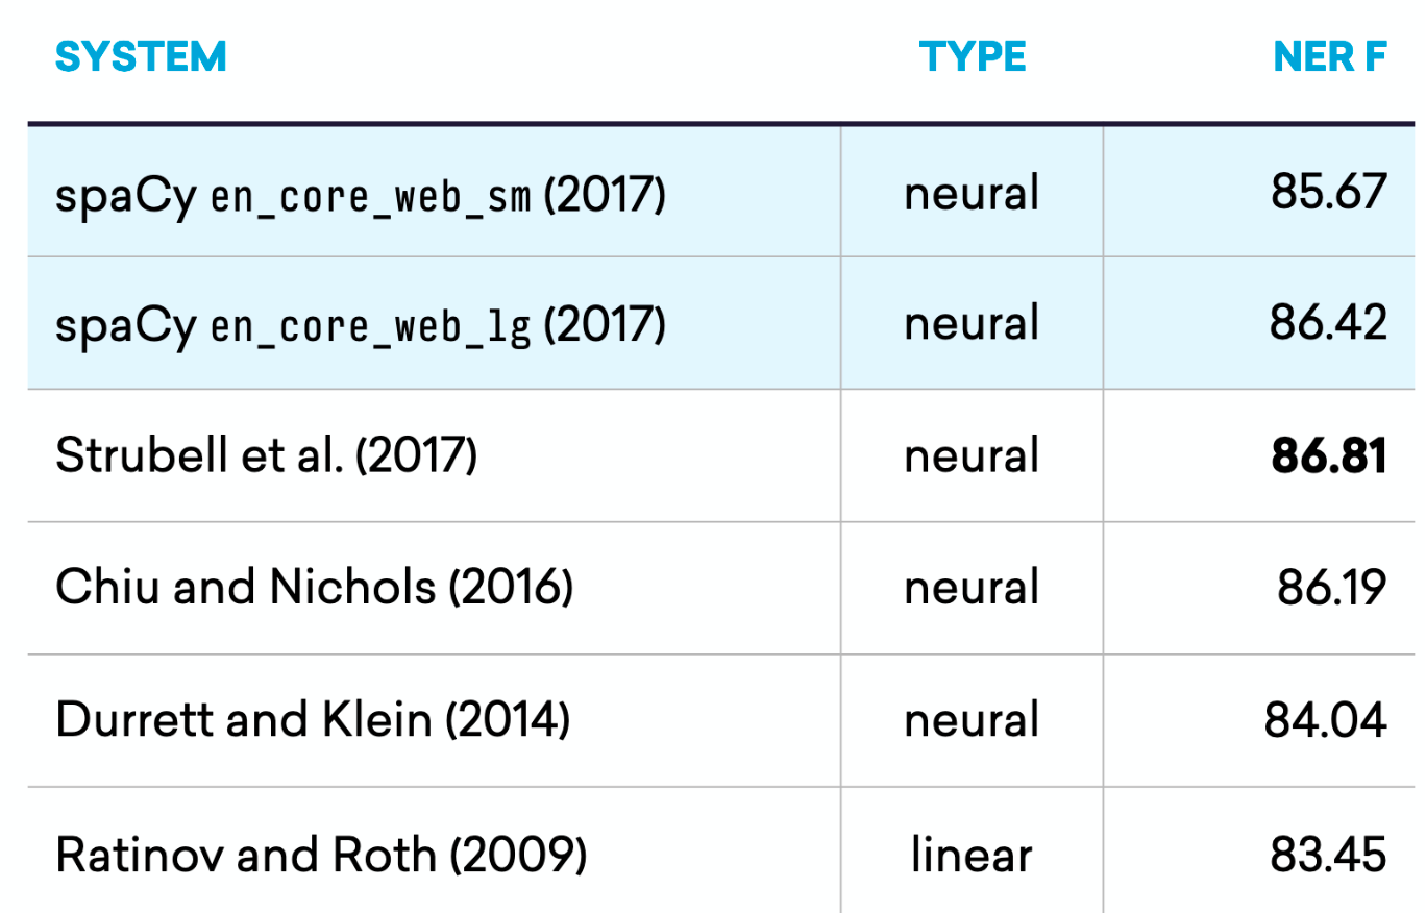
\includegraphics{assets/state-of-the-art_difficulties.pdf} 

}

\caption{Principales avances del estado del arte para NER en los últimos años}\label{fig:spacy-algos}
\end{figure}

Las razones por las cuales esto ocurre escapa el alcance de este trabajo pero se pueden resumir bajo la ley de los rendimientos decrecientes. Se necesita mucho esfuerzo académico para obtener una mejora marginal en el estado del arte actual.

Es por esto que resulta interesante analizar que otro tipo de problemas podemos atacar en este trabajo.

\hypertarget{dominios-del-problema}{%
\paragraph{Dominios del problema}\label{dominios-del-problema}}

Existe un hilo conductor en el que todas las investigaciones mencionadas en la figura \ref{fig:spacy-algos} coinciden; incluso los sistemas NER más avanzadas son frágiles, dado que los sistemas NER desarrollados para un dominio no suelen comportarse bien en otros dominios (Poibeau \& Kosseim, \protect\hyperlink{ref-Poibeau2000ProperNE}{2000}). La puesta a punto de un sistema NER para un nuevo dominio conlleva un esfuerzo considerable. Esto es cierto para modelos basados en reglas y para sistemas estadísticos.

Se entiende por dominio a todos los textos que en su conjunto forman un corpus común. Ejemplos de estos son \enquote{Noticias periodísticas}, \enquote{Textos jurídicos}, \enquote{Reportes militares}, \enquote{Papers académicos}, etc.

\hypertarget{los-datos-son-el-problema}{%
\subsection{Los datos son el problema}\label{los-datos-son-el-problema}}

Por todo lo mencionado, es evidente que el cuello de botella para el avance de esta y muchas areas de la IA es el la captura de datos, no los algoritmos (Montani, \protect\hyperlink{ref-montani_AI}{2016}).

En particular para el estado actual del arte de \texttt{NER} es necesario tener el cuerpo de textos a analizar (Corpus) tagueado de tal manera que se conozcan previamente los nombres y tipos de entidades de un subconjunto de textos para inferir sobre el resto.

Este aprendizaje se carga en lo que se reconoce como un \enquote{Modelo estadístico} y es a ese model al que se le pide inferir nuevos resultados. En nuestra experiencia los modelos pre-entrenados de las diferentes plataformas / librerias / frameworks y trabajos académicos resultan siempre insuficientes para el uso en producción de los mismos.

De esta manera queda bien definido el problema que queremos atacar (y el título de este trabajo)

\begin{quote}
Creación eficiente de modelos estadísticos para detección automática y precisa de entidades nombradas
\end{quote}

Para este fin se creó un sistema informático que permitirá obtener resultados a la altura de de las soluciones del estado del arte para cualquier corpus de documentos que posea una cantidad necesaria de datos.

\newpage

\hypertarget{state-of-art}{%
\section{Estado del arte}\label{state-of-art}}

El análisis del estado del arte fue basado en la definición del problema.

\hypertarget{stack-de-software}{%
\subsection{Stack de software}\label{stack-de-software}}

Python es el lenguaje más utilizado para resolver problemas de Machine Learning, en especial NLP (``The state of the octoverse,'' \protect\hyperlink{ref-github_machine_learning}{2019})

Spacy es el framework mejor ranqueado para la tarea de NLP (``The state of the octoverse,'' \protect\hyperlink{ref-github_machine_learning}{2019}) y sabemos por la Figura \ref{fig:spacy-algos} que obtiene resultados a-la-par del estado del arte actual.

Además la implementación de spacy es robusta y orientada a la creación de apliciones para producción, a diferencia de muchas otras librerías de NLP que sólo se utilizan con fines académicos.

\hypertarget{el-pipeline}{%
\subsection{El pipeline}\label{el-pipeline}}

Todas las operaciones de analisis de lenguaje natural sobre textos no estructurados, tienen como primer paso el de separar el los mismos en tokens. Luego, el documento se procesa en varios pasos diferentes que consisten en el \enquote{pipeline de procesamiento}. Usualmente los pasos consisten en un etiquetador, un analizador sintáctico y un reconocedor de entidades en el caso de NER.

Cada componente del pipeline devuelve el Doc procesado, que luego se pasa al siguiente componente.

\begin{figure}[H]

{\centering 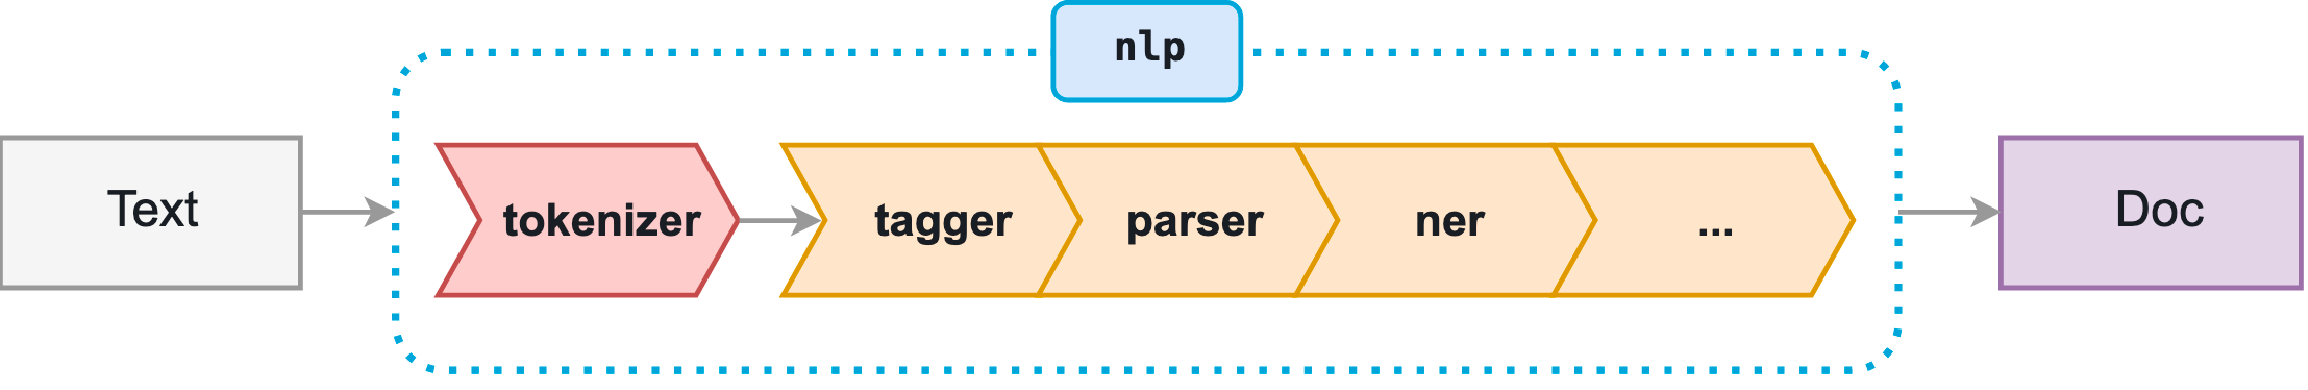
\includegraphics{assets/spacy_pipeline.pdf} 

}

\caption{Pipeline standard para los algoritmos de NER}\label{fig:spacy-pipeline}
\end{figure}

En este capítulo esturiaremos la morfología de dicho pipeline.

\hypertarget{algoritmo-de-tokenizaciuxf3n}{%
\subsection{Algoritmo de tokenización}\label{algoritmo-de-tokenizaciuxf3n}}

Para tokenizar un texto de manera correcta no basta con separar el mismo en espacios. Dependiendo el lenguaje que se esté estudiando, existen \enquote{excepciones} a esta regla y otros caracteres que representan separaciones entre tokens segun el contexto de los mismos.

En particular, spaCy posee algoritmo de tokenización inteligente que puede ser resumido de la siguiente manera:

\begin{enumerate}
\def\labelenumi{\arabic{enumi}.}
\tightlist
\item
  Iterar sobre subcadenas separadas por espacios en blanco.
\item
  Compruebar si existe una regla definida explícitamente para esta subcadena. Si existe, usarla.
\item
  De lo contrario, intentar consumir un prefijo. Si consumimos un prefijo, regrese al punto\#2, para que los casos especiales siempre tengan prioridad.
\item
  Si no se puede consumir un prefijo, intente consumir un sufijo y luego regrese al punto \#2.
\item
  Si no se puede consumir un prefijo ni un sufijo, buscar un caso especial.
\item
  Buscar una coincidencia de token
\item
  Buscar \enquote{infijos} - cosas como guiones, etc. y dividir la subcadena en tokens en todos los infijos.
\item
  Una vez que no se pueda consumir más de la cadena, tratarla como un token único.
\end{enumerate}

Ejemplo:

\begin{figure}[H]

{\centering 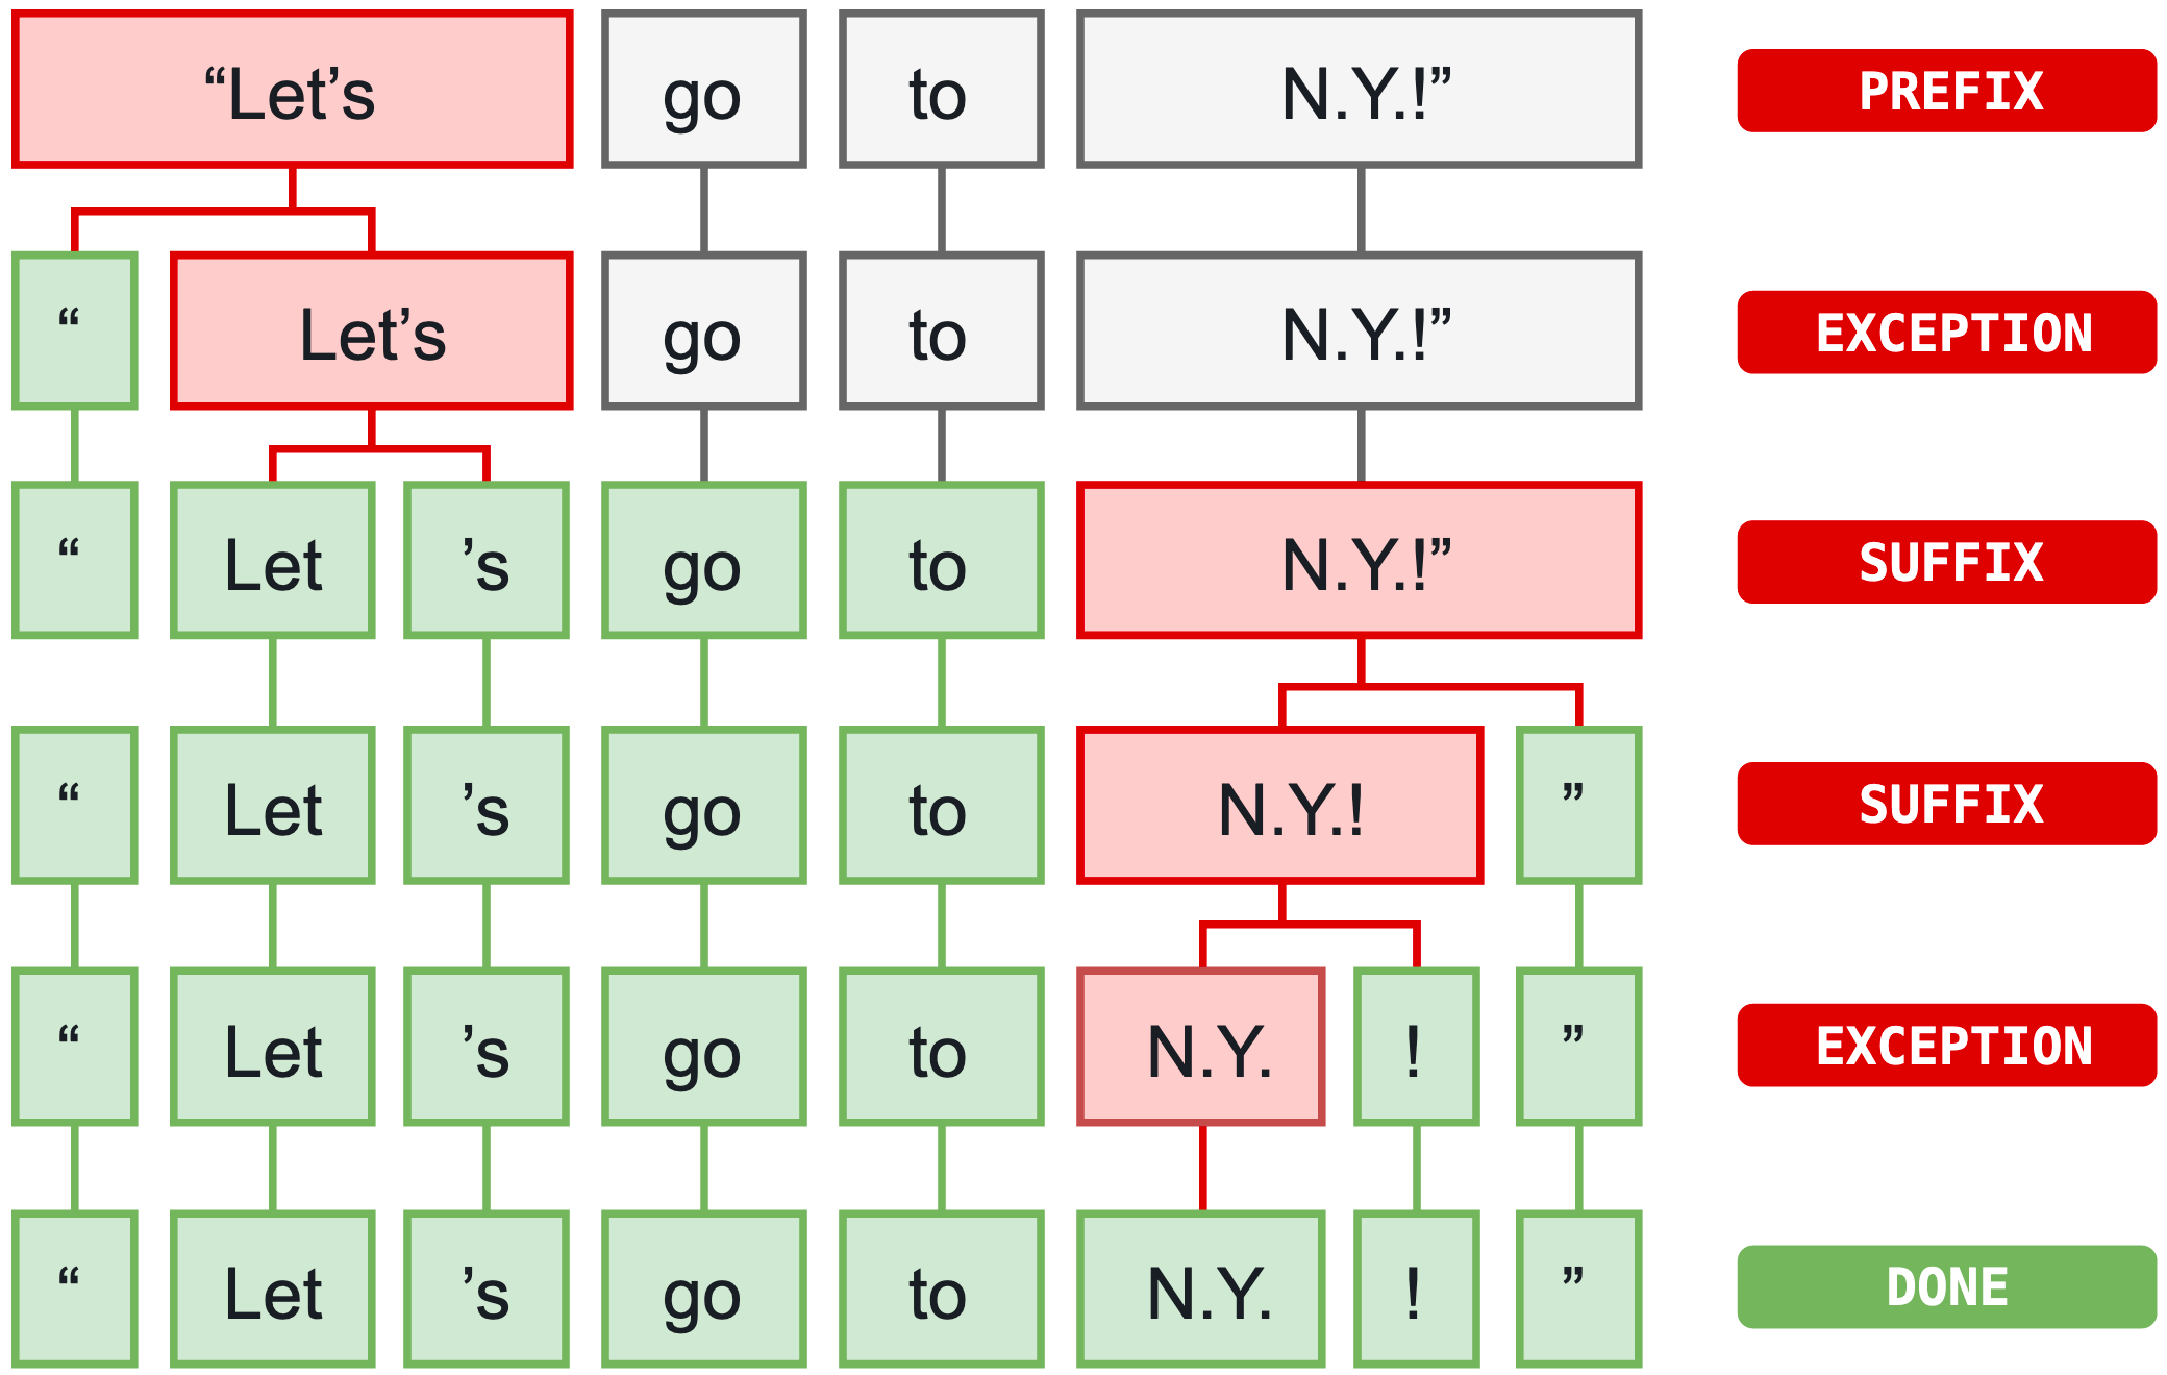
\includegraphics{assets/spacy_tokenization.pdf} 

}

\caption{Transiciones del modelo Stack-LSTM indicando la acción aplicada y el estado resultante.}\label{fig:spacy-tokenization}
\end{figure}

\hypertarget{reconocimiento-de-entidades-1}{%
\subsection{Reconocimiento de entidades}\label{reconocimiento-de-entidades-1}}

\hypertarget{modelos-basados-en-reglas}{%
\subsubsection{Modelos basados en reglas}\label{modelos-basados-en-reglas}}

Antes de entrar en detalles de cómo trabaja el modelo estadístico de spacy y entender sus fortalezas es importante esbozar brevemente el grupo de algorítmos más \enquote{naive} posible. El de los modelos basados en reglas fijas.

En estos modelos se implementan reglas finitas o expresiones regulares para la detección de las entidades. Las principales limitaciones de este enfoque son:

\begin{itemize}
\tightlist
\item
  \textbf{Mucho trabajo manua}l: el sistema RB exige un profundo conocimiento del dominio, así como mucho trabajo manual.
\item
  \textbf{Consumo de tiempo}: la generación de reglas para un sistema complejo es bastante difícil y requiere mucho tiempo.
\item
  \textbf{Menor capacidad de aprendizaje}: el sistema generará el resultado según las reglas, por lo que la capacidad de aprendizaje del sistema por sí mismo es baja.
\item
  \textbf{Dominios complejos}: si el corpus demasiado complejo, la creación del sistema RB puede llevar mucho tiempo y análisis. La identificación de patrones complejos es una tarea desafiante en el enfoque RB.
\end{itemize}

\hypertarget{el-enfoque-de-spacy}{%
\subsubsection{El enfoque de spaCy}\label{el-enfoque-de-spacy}}

Cuando se busca mejorar el aprendizaje automático, generalmente se piensa en la eficiencia y la precisión, pero la dimensión más importante es la generalidad.

La mayoría de los problemas de \texttt{NLP} pueden reducirse a problemas de aprendizaje automático que toman uno o más textos como entrada. Si podemos transformar estos textos en vectores, podemos reutilizar soluciones de aprendizaje profundo (\emph{deep-learning}) de propósito general.

\hypertarget{muxe1quina-de-estados}{%
\paragraph{Máquina de estados}\label{muxe1quina-de-estados}}

Experimentos en inglés, holandés, alemán y español muestran que se pueden obtener resultados a-la-par del estado del arte utilizando un autómata finito determinístico de pila en conjunción con una red neuronal (Lample, Ballesteros, Subramanian, Kawakami, \& Dyer, \protect\hyperlink{ref-DBLP:journalsux2fcorrux2fLampleBSKD16}{2016})

Este autómata de pila es el nexo entre la Red Neuronal Convolucional (CNN) que contiene el modelo estadístico para predecir entidades y el texto completo. No se envía el texto entero como input a dicha red, sino que se van enviando cada uno de los estados en los que el autómata de pila se mueve para ir generando entidades con una herística del tipo \emph{greedy}.

Las posibles acciones de transición de este autómata son las siguientes:

\begin{figure}[H]

{\centering 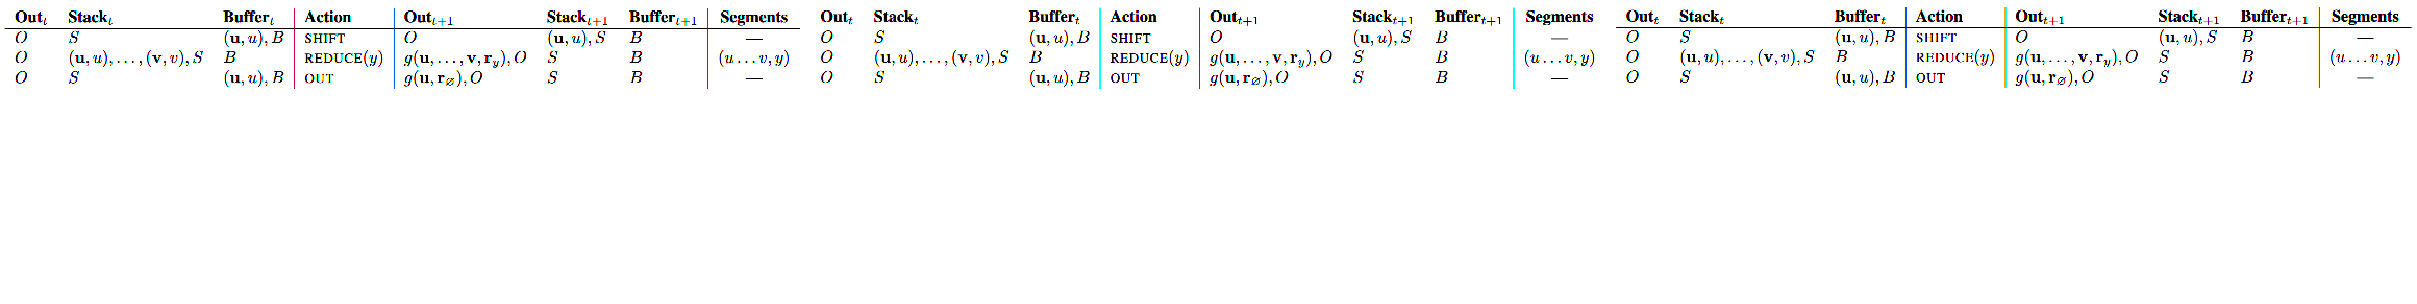
\includegraphics{assets/lampe_1.pdf} 

}

\caption{Transiciones del modelo Stack-LSTM indicando la acción aplicada y el estado resultante.}\label{fig:lampe-1}
\end{figure}

\begin{itemize}
\tightlist
\item
  SHIFT: consume una token del input y al mueve al stack para generar una nueva entidad.
\item
  REDUCE: mueve el stack actual al output tagueado como entity.
\item
  OUT: consume una token del input y la mueve sl output directamente.
\end{itemize}

Para saber que acción tomar se consulta el modelo estadístico.En la siguiente figura se puede ver un ejemplo de cómo se recorre una oración bajo el stack propuesto:

\begin{figure}[H]

{\centering 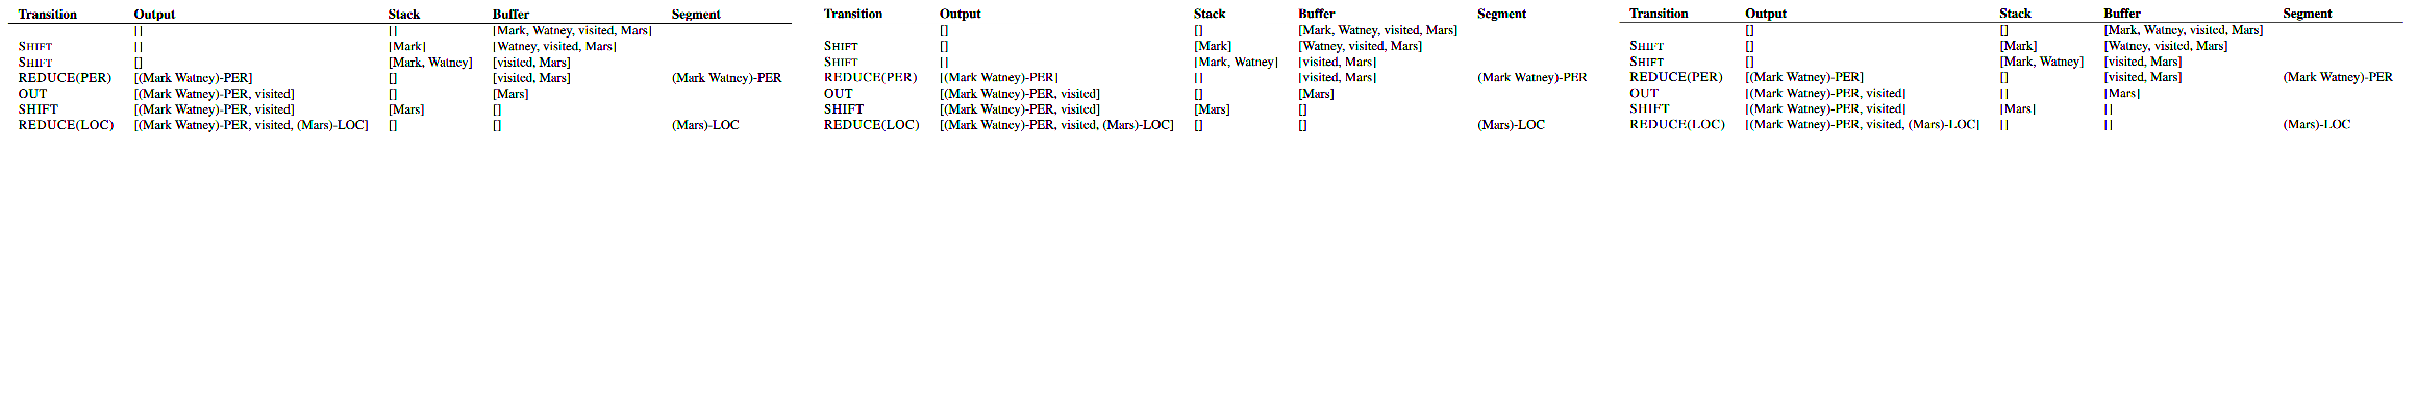
\includegraphics{assets/lampe_2.pdf} 

}

\caption{Secuencia de tranciciones para el ejemplo "Mark Watney visited Mars" en el modelo de Stack-LSTM.}\label{fig:lampe-2}
\end{figure}

\begin{itemize}
\tightlist
\item
  Primero se empieza con un stack vacío.
\item
  Se consume \enquote{Mark} y la CNN predice que es una posible Persona. Lo envia al stack.
\item
  Se consume \enquote{Watney} y la CNN predice que es una posible continuación de Persona. Lo envia al stack.
\item
  Se consume \enquote{visited} y la CNN predice que esto no forma parte de una entidad. Por lo tanto antes se REDUCE la entidad \enquote{Mark Watney} del stack actual.
\item
  Análogamente se detecta la entidad \enquote{Mars}
\end{itemize}

\hypertarget{el-modelo-estaduxedstico-deep-learning}{%
\subsection{\texorpdfstring{El modelo estadístico \enquote{deep-learning}}{El modelo estadístico ``deep-learning''}}\label{el-modelo-estaduxedstico-deep-learning}}

El modelo de deep learning elegido para trabajar es el de spaCy. Consiste en una Red Neuronal convolucional que predice las entidades.

Redes neuronales convolucionales
\url{https://es.wikipedia.org/wiki/Redes_neuronales_convolucionales}

Para entender cómo funciona dicha red neuronal, se puede definir el proceso en 4 etapas que transforman la información entre diferentes estados

\begin{figure}[H]

{\centering 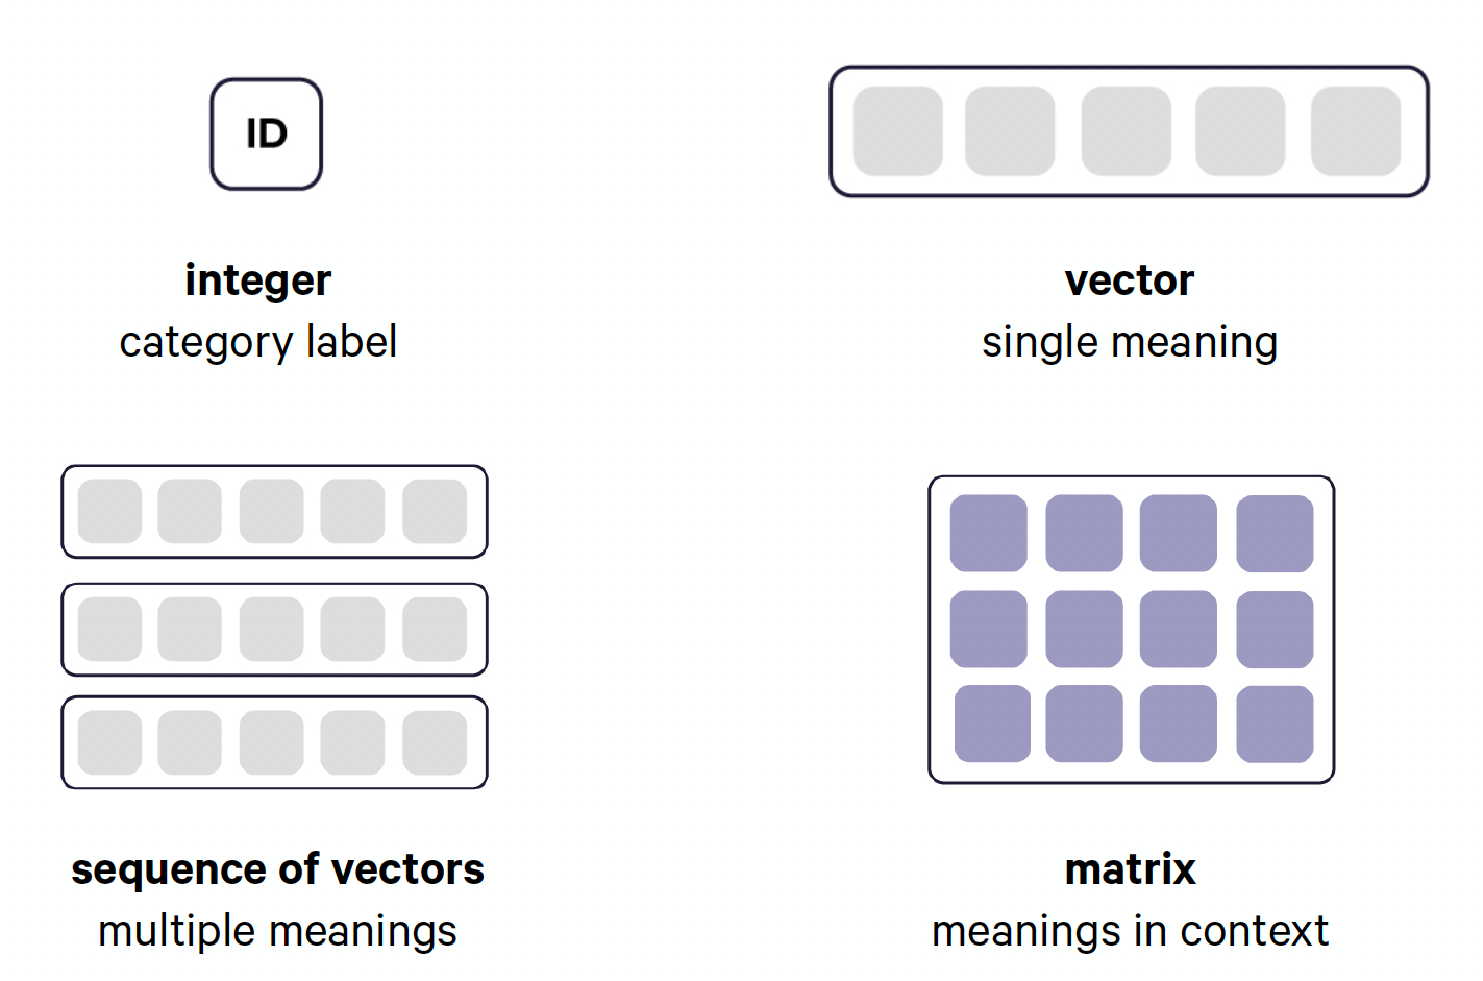
\includegraphics{assets/deep-learning-formula-nlp_shapes.pdf} 

}

\caption{Estados posibles para las diferentes etapas de la CNN}\label{fig:formula-shapes}
\end{figure}

\hypertarget{embed}{%
\subsubsection{embed}\label{embed}}

\begin{quote}
Problema: \enquote{todas las palabras sin iguales para la computadora}
\end{quote}

La idea de \emph{word embeddings} es la de \enquote{embeber} el conjunto de tokens que componen términos con información adicional.

\begin{figure}[H]

{\centering 
\includegraphics{assets/deep-learning-formula-nlp_embed.pdf} 

}

\caption{TODO: embed}\label{fig:formula-embed}
\end{figure}

\hypertarget{encode}{%
\subsubsection{encode}\label{encode}}

\begin{figure}[H]

{\centering 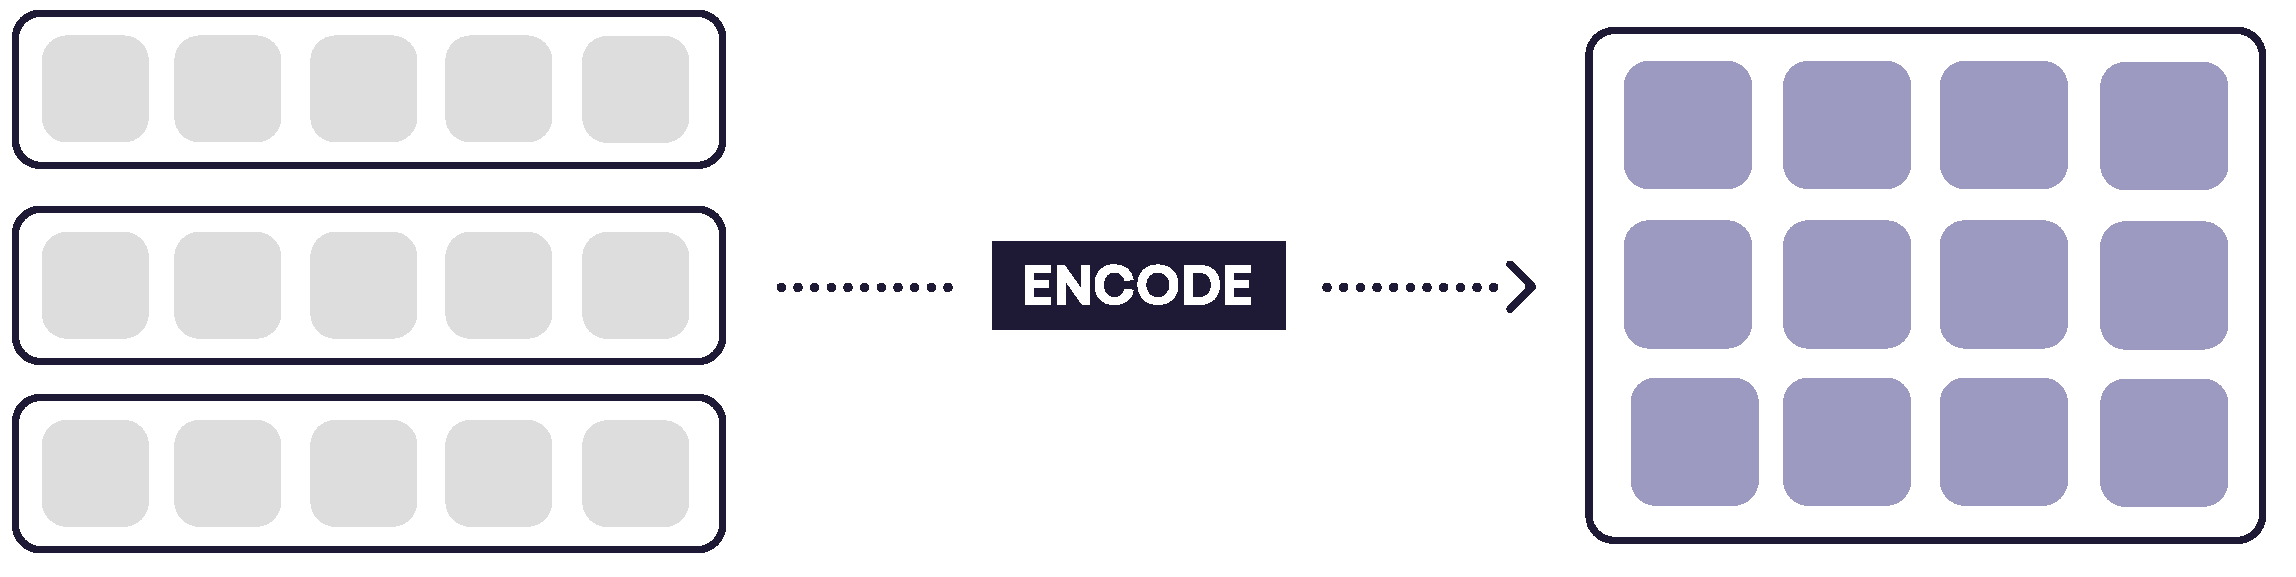
\includegraphics{assets/deep-learning-formula-nlp_encode.pdf} 

}

\caption{TODO: encode}\label{fig:formula-encode}
\end{figure}

\hypertarget{attend}{%
\subsubsection{attend}\label{attend}}

\begin{figure}[H]

{\centering 
\includegraphics{assets/deep-learning-formula-nlp_attend.pdf} 

}

\caption{TODO: attend}\label{fig:formula-attend}
\end{figure}

\hypertarget{predict}{%
\subsubsection{predict}\label{predict}}

\begin{figure}[H]

{\centering 
\includegraphics{assets/deep-learning-formula-nlp_predict.pdf} 

}

\caption{TODO: predict}\label{fig:formula-predict}
\end{figure}

Here is a review of existing methods.

\hypertarget{subword-features}{%
\subsection{Subword features}\label{subword-features}}

Yes, spaCy's NER (and other models) uses subword features, although it doesn't use a character-based CNN to extract them. Instead, the word vectors are learned by concatenating embeddings of NORM, PREFIX, SUFFIX and SHAPE lexical attributes. A hidden layer is then used to allow a non-linear combination of the information in these concatenated vectors. The function for this can be found in spacy.\_ml.Tok2Vec.

The best reference for this embedding strategy is currently the NER algorithm video: \url{https://www.youtube.com/watch?v=sqDHBH9IjRU}

To add to @ honnibal's comment above, there's also a section in the API docs that describes the neural network model architecture in more detail: \url{https://spacy.io/api/\#nn-model}

\hypertarget{statistical-entity-recognition-model}{%
\subsection{statistical entity recognition model}\label{statistical-entity-recognition-model}}

\hypertarget{word-vectors}{%
\subsection{Word vectors}\label{word-vectors}}

\[\vec{king} - \vec{man} + \vec{woman} \approx \vec{queen}\]

(Ethayarajh, Duvenaud, \& Hirst, \protect\hyperlink{ref-ethayarajh-etal-2019-towards}{2019})

\begin{figure}[H]

{\centering 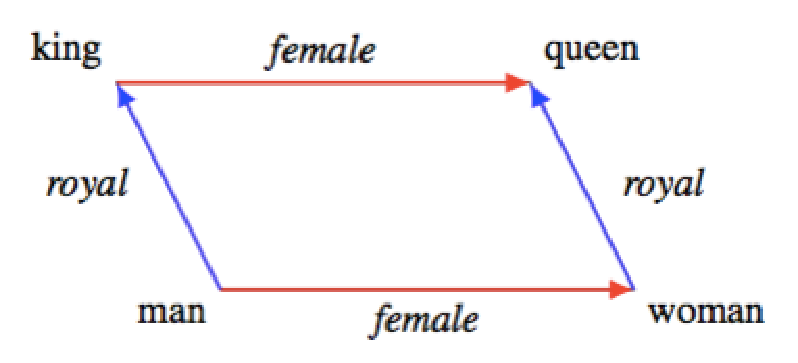
\includegraphics{assets/parallelogram.pdf} 

}

\caption{Parallelogram structure in the vector space (by definition)}\label{fig:vec-parallelogram}
\end{figure}

\url{https://www.youtube.com/watch?v=sqDHBH9IjRU}
SPACY'S ENTITY RECOGNITION MODEL: incremental parsing with Bloom embeddings \& residual CNNs

\url{https://github.com/explosion/talks/blob/master/2018-04-12_Embed-Encode-Attend-Predict.pdf}

\newpage

\hypertarget{implementation}{%
\section{NERd (Implementación)}\label{implementation}}

Definido el problema, queda claro que la creación de un modelo entrenado es de vital importancia para cualquier problema de tagueo de entidades.
Es por ello que en el presente proyecto final hemos creado una herramienta para el entrenamiento eficiente de modelos estadísticos así como también una interfaz y API para poder consultar entidades.
El nombre de esta herramienta es \textbf{NERd}, sigla cuyo significado en inglés es \emph{\textbf{N}amed \textbf{E}ntity \textbf{R}ecognition \textbf{D}uh}\footnote{Expresión de obviedad. \emph{Used to express your belief that what was said was extremely obvious} (``Duh definition,'' \protect\hyperlink{ref-cambridge_duh}{2019})}!

Para organizar este capítulo vamos a realizar una descripción basada en el modelo de vistas de arquitectura 4+1.

\begin{figure}[H]

{\centering 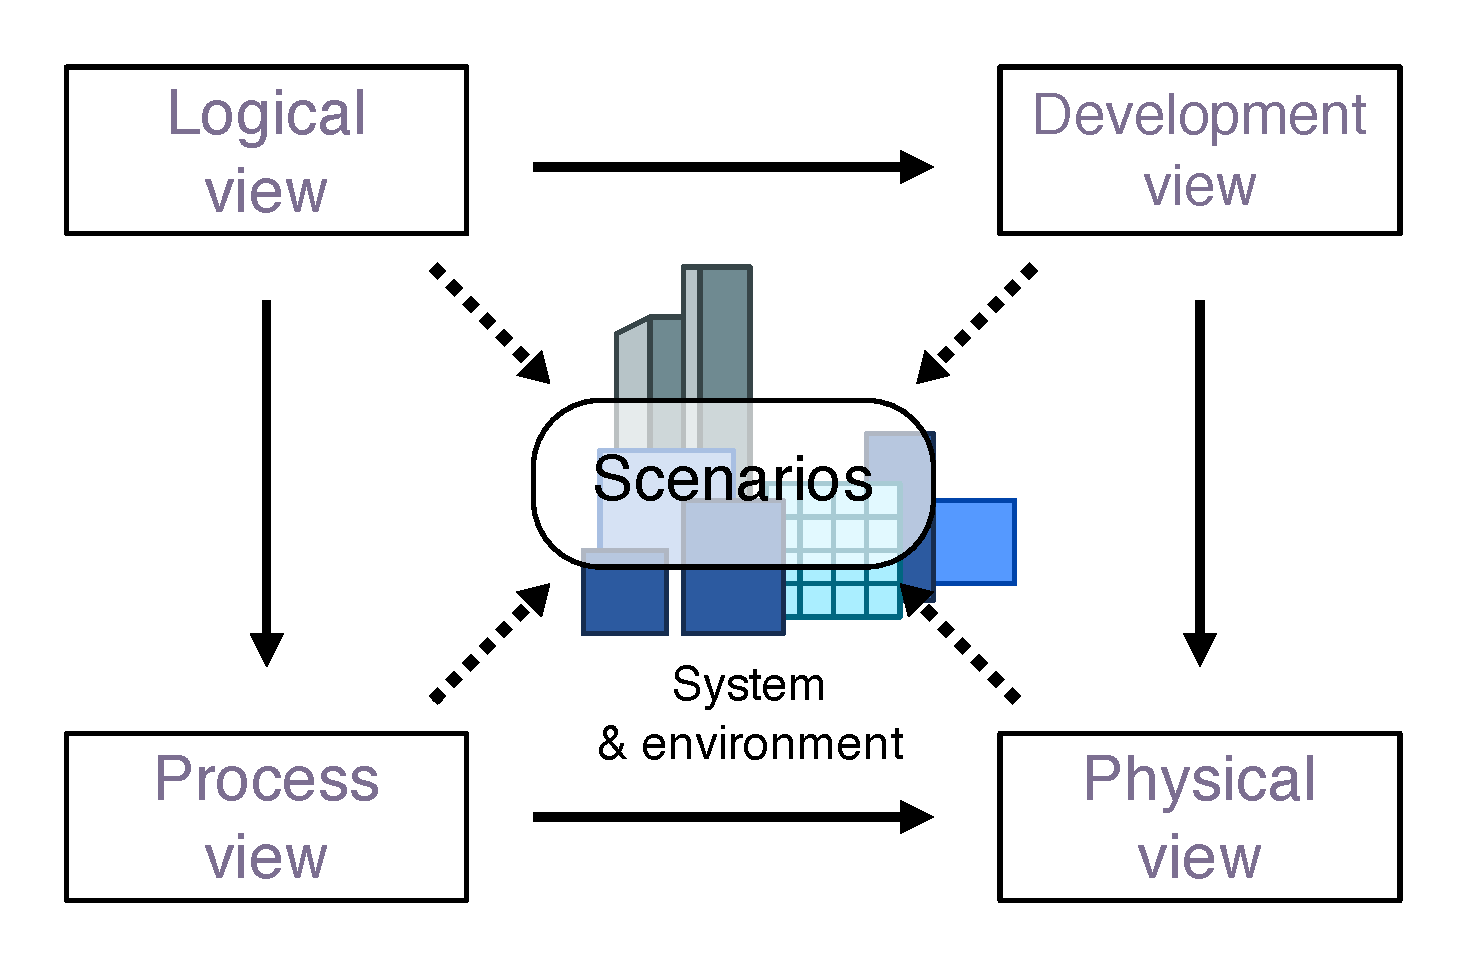
\includegraphics{assets/4+1_Architectural_View_Model.pdf} 

}

\caption{Ilustración de arquitectura 4+1}\label{fig:arq41}
\end{figure}

Este modelo nos permite describir la aplicación de una manera genérica y ordenada.

\begin{quote}
\emph{The \enquote{4+1} view model is rather \enquote{generic}: other notations and tools can be used, other design methods can be used, especially for the logical and process decompositions, but we have indicated the ones we have used with success.}

\hfill --- (Kruchten, \protect\hyperlink{ref-Kruchten:1995:VMA:624610.625529}{1995})
\end{quote}

\hypertarget{vista-luxf3gica}{%
\subsection{Vista lógica}\label{vista-luxf3gica}}

\begin{quote}
La vista lógica se refiere a la funcionalidad que el sistema proporciona a los usuarios finales.
\end{quote}

A continuación detallamos distintas partes del servicio NERd así como también de la interfaz de entrenamiento.

\hypertarget{servicio}{%
\subsubsection{Servicio}\label{servicio}}

El acceso al servicio se realiza mediante un API REST que se auto-documenta debido a implementar la especificación de OpenAPI. A continuación detallamos los endpoints.

\hypertarget{autenticaciuxf3n}{%
\paragraph{Autenticación}\label{autenticaciuxf3n}}

Rutas del API dedicadas a la autenticación de usuarios.

\begin{itemize}
\tightlist
\item
  \textbf{POST} \emph{/api/auth/register}

  \begin{itemize}
  \tightlist
  \item
    Registrar un usuario nuevo.
  \end{itemize}
\item
  \textbf{POST} \emph{/api/auth/token}

  \begin{itemize}
  \tightlist
  \item
    Genera un nuevo token de acceso y refresco con credenciales.
  \item
    Utilizado para la funcionalidad de \emph{login}
  \end{itemize}
\item
  \textbf{POST} \emph{/api/auth/refresh}

  \begin{itemize}
  \tightlist
  \item
    Refresca el token de acceso.
  \item
    Utilizado cuando un token de acceso caducó.
  \end{itemize}
\end{itemize}

\hypertarget{usuarios}{%
\paragraph{Usuarios}\label{usuarios}}

Conjunto de operaciones relacionadas con los usuarios del sistema.

\begin{itemize}
\tightlist
\item
  \textbf{GET} \emph{/api/users}

  \begin{itemize}
  \tightlist
  \item
    Lista de usuarios existentes
  \item
    Separa los resultados en páginas
  \end{itemize}
\item
  \textbf{GET} \emph{/api/users/top5}

  \begin{itemize}
  \tightlist
  \item
    Lista de los 5 usuarios con más entrenamientos
  \end{itemize}
\item
  \textbf{GET} \emph{/api/users/me}

  \begin{itemize}
  \tightlist
  \item
    Retorna la información del usuario logueado
  \end{itemize}
\item
  \textbf{PATCH} \emph{/api/users/me}

  \begin{itemize}
  \tightlist
  \item
    Actualiza la información del usuario logueado
  \end{itemize}
\item
  \textbf{GET} \emph{/api/users/me/trainings}

  \begin{itemize}
  \tightlist
  \item
    Retorna los entrenamientos del usuario logueado
  \item
    Separa los resultados en páginas
  \end{itemize}
\item
  \textbf{GET} \emph{/api/users/\{user\_id\}}

  \begin{itemize}
  \tightlist
  \item
    Retorna la información del usuario especificado por \emph{user\_id}
  \end{itemize}
\item
  \textbf{PATCH} \emph{/api/users/\{user\_id\}}

  \begin{itemize}
  \tightlist
  \item
    Actualiza la información del usuario especificado por \emph{user\_id}
  \end{itemize}
\item
  \textbf{DELETE} \emph{/api/users/\{user\_id\}}

  \begin{itemize}
  \tightlist
  \item
    Borra al usuario especificado por \emph{user\_id}
  \end{itemize}
\item
  \textbf{GET} \_/api/users/\{user\_id\}/trainings

  \begin{itemize}
  \tightlist
  \item
    Retorna los entrenamientos del usuario especificado
  \end{itemize}
\end{itemize}

\hypertarget{roles}{%
\paragraph{Roles}\label{roles}}

\begin{itemize}
\tightlist
\item
  \textbf{GET} \emph{/api/roles}

  \begin{itemize}
  \tightlist
  \item
    Retorna la lista de todos los roles asignables a usuarios del sistema
  \end{itemize}
\end{itemize}

\hypertarget{corpus}{%
\paragraph{Corpus}\label{corpus}}

Rutas dedicadas a operaciones con el corpus del sistema.

\begin{itemize}
\tightlist
\item
  \textbf{GET} \emph{/api/corpus/\{text\_id\}}

  \begin{itemize}
  \tightlist
  \item
    Retorna los detalles del texto especificado por \emph{text\_id}
  \end{itemize}
\item
  \textbf{DELETE} \emph{/api/corpus/\{text\_id\}}

  \begin{itemize}
  \tightlist
  \item
    Borra un texto especificado por \emph{text\_id} del corpus
  \end{itemize}
\item
  \textbf{GET} \emph{/api/corpus/\{text\_id\}/trainings}

  \begin{itemize}
  \tightlist
  \item
    Retorna la lista de entrenamientos proporcionados por los usuarios sobre las entidades en el texto
  \end{itemize}
\item
  \textbf{PUT} \emph{/api/corpus/\{text\_id\}/trainings}

  \begin{itemize}
  \tightlist
  \item
    Agrega un entrenamiento para el texto con id \emph{text\_id}
  \end{itemize}
\item
  \textbf{POST} \emph{/api/corpus/upload}

  \begin{itemize}
  \tightlist
  \item
    Permite agregar textos de manera masiva al sistema
  \item
    Acepta una lista de archivos .txt donde cada línea es un texto a agregar
  \item
    Los archivos deben ser UTF-8
  \end{itemize}
\item
  \textbf{GET} \emph{/api/corpus}

  \begin{itemize}
  \tightlist
  \item
    Lista de textos cargados en el sistema para entrenamiento
  \item
    Separa los resultados en páginas
  \end{itemize}
\item
  \textbf{POST} \emph{/api/corpus}

  \begin{itemize}
  \tightlist
  \item
    Agrega un texto al sistema para entrenamiento
  \end{itemize}
\end{itemize}

\hypertarget{snapshots}{%
\paragraph{Snapshots}\label{snapshots}}

Conjunto de operaciones relacionadas con los snapshots y workers.

\begin{itemize}
\tightlist
\item
  \textbf{GET} \emph{/api/snapshots}

  \begin{itemize}
  \tightlist
  \item
    Listado de los snapshots disponibles
  \item
    Separa los resultados en páginas
  \end{itemize}
\item
  \textbf{GET} \emph{/api/snapshots/\{snapshot\_id\}}

  \begin{itemize}
  \tightlist
  \item
    Retorna información (tipos de entidades, fecha de creación, fecha de entrenamiento, etc.) sobre un snapshot específico
  \end{itemize}
\item
  \textbf{DELETE} \emph{/api/snapshots/\{snapshot\_id\}}

  \begin{itemize}
  \tightlist
  \item
    Borra un snapshot con el id especificado
  \end{itemize}
\item
  \textbf{POST} \emph{/api/snapshots/\{snapshot\_id\}/force-train}

  \begin{itemize}
  \tightlist
  \item
    Envía la tarea de entrenamiento a los workers que tienen el snapshot \emph{snapshot\_id} cargado.
  \end{itemize}
\item
  \textbf{POST} \emph{/api/snapshots/\{snapshot\_id\}/force-untrain}

  \begin{itemize}
  \tightlist
  \item
    Envía la tarea de desentrenar a los workers que tienen el snapshot \emph{snapshot\_id} cargado.
  \end{itemize}
\item
  \textbf{GET} \emph{/api/snapshots/current}

  \begin{itemize}
  \tightlist
  \item
    Retorna información sobre el snapshot actual
  \end{itemize}
\item
  \textbf{PUT} \emph{/api/snapshots/current}

  \begin{itemize}
  \tightlist
  \item
    Crea un nuevo snapshot con la información provista
  \end{itemize}
\end{itemize}

\hypertarget{reconocimiento-de-entidades-nombradas}{%
\paragraph{Reconocimiento de Entidades Nombradas}\label{reconocimiento-de-entidades-nombradas}}

Conjunto de operaciones relacionadas al \emph{Reconocimiento de Entidades Nombradas}

\begin{itemize}
\tightlist
\item
  \textbf{GET} \emph{/api/ner/train}

  \begin{itemize}
  \tightlist
  \item
    Retorna un texto para que un usuario del sistema revise si está correctamente inferido
  \item
    Únicamente retorna textos que el usuario logueado no haya corregido ya
  \end{itemize}
\item
  \textbf{GET} \emph{/api/ner/compare/\{first\_snapshot\}/\{second\_snapshot\}}

  \begin{itemize}
  \tightlist
  \item
    Compara el \emph{Reconocimiento de Entidades Nombradas} entre dos snapshots distintos
  \end{itemize}
\item
  \textbf{POST} \emph{/api/ner/current/parse}

  \begin{itemize}
  \tightlist
  \item
    Retorna un documento Spacy para un texto dado utilizando el snapshot actual
  \end{itemize}
\item
  \textbf{POST} \emph{/api/ner/\{snapshot\_id\}/parse}

  \begin{itemize}
  \tightlist
  \item
    Retorna un documento Spacy para un texto dado utilizando el snapshot especificado
  \end{itemize}
\item
  \textbf{POST} \emph{/api/ner/current/entities}

  \begin{itemize}
  \tightlist
  \item
    Retorna la lista de \emph{Entidades Nombradas} para un texto dado utilizando el modelo actual
  \end{itemize}
\item
  \textbf{POST} \emph{/api/ner/\{snapshot\_id\}/entities}

  \begin{itemize}
  \tightlist
  \item
    Retorna la lista de \emph{Entidades Nombradas} para un texto dado utilizando el modelo especificado
  \end{itemize}
\end{itemize}

\hypertarget{entrenamientos}{%
\paragraph{Entrenamientos}\label{entrenamientos}}

\begin{itemize}
\tightlist
\item
  \textbf{DELETE} \emph{/api/trainings/\{training\_id\}}

  \begin{itemize}
  \tightlist
  \item
    Borra un entrenamiento
  \end{itemize}
\end{itemize}

\hypertarget{workers}{%
\paragraph{Workers}\label{workers}}

\begin{itemize}
\tightlist
\item
  \textbf{GET} \emph{/api/workers/}

  \begin{itemize}
  \tightlist
  \item
    Lista de los workers disponibles
  \end{itemize}
\item
  \textbf{POST} \emph{/api/workers/reassign}

  \begin{itemize}
  \tightlist
  \item
    Reasigna un trabajador de un a versión de snapshot a otra
  \end{itemize}
\end{itemize}

\hypertarget{web}{%
\subsubsection{Web}\label{web}}

La página web de \emph{NERd} está enfocada en las tareas de mantenimiento de los servicios ofrecidos por el \emph{API} así como también ofrece de interfaces que permiten a usuarios del sistema corregir de manera eficiente el modelo de inferencia.

\hypertarget{inicio}{%
\paragraph{Inicio}\label{inicio}}

Pantalla de inicio donde se encuentran accesos rápidos para entrenar el modelo o para poder buscar entidades en textos.
También se encuentra aquí una lista de los 5 usuarios que más contribuyeron a entrenar el modelo. Detrás de esta funcionalidad se busca generar un espíritu competitivo entre los usuarios para que los mismos busquen contribuir más.

\begin{figure}[H]

{\centering 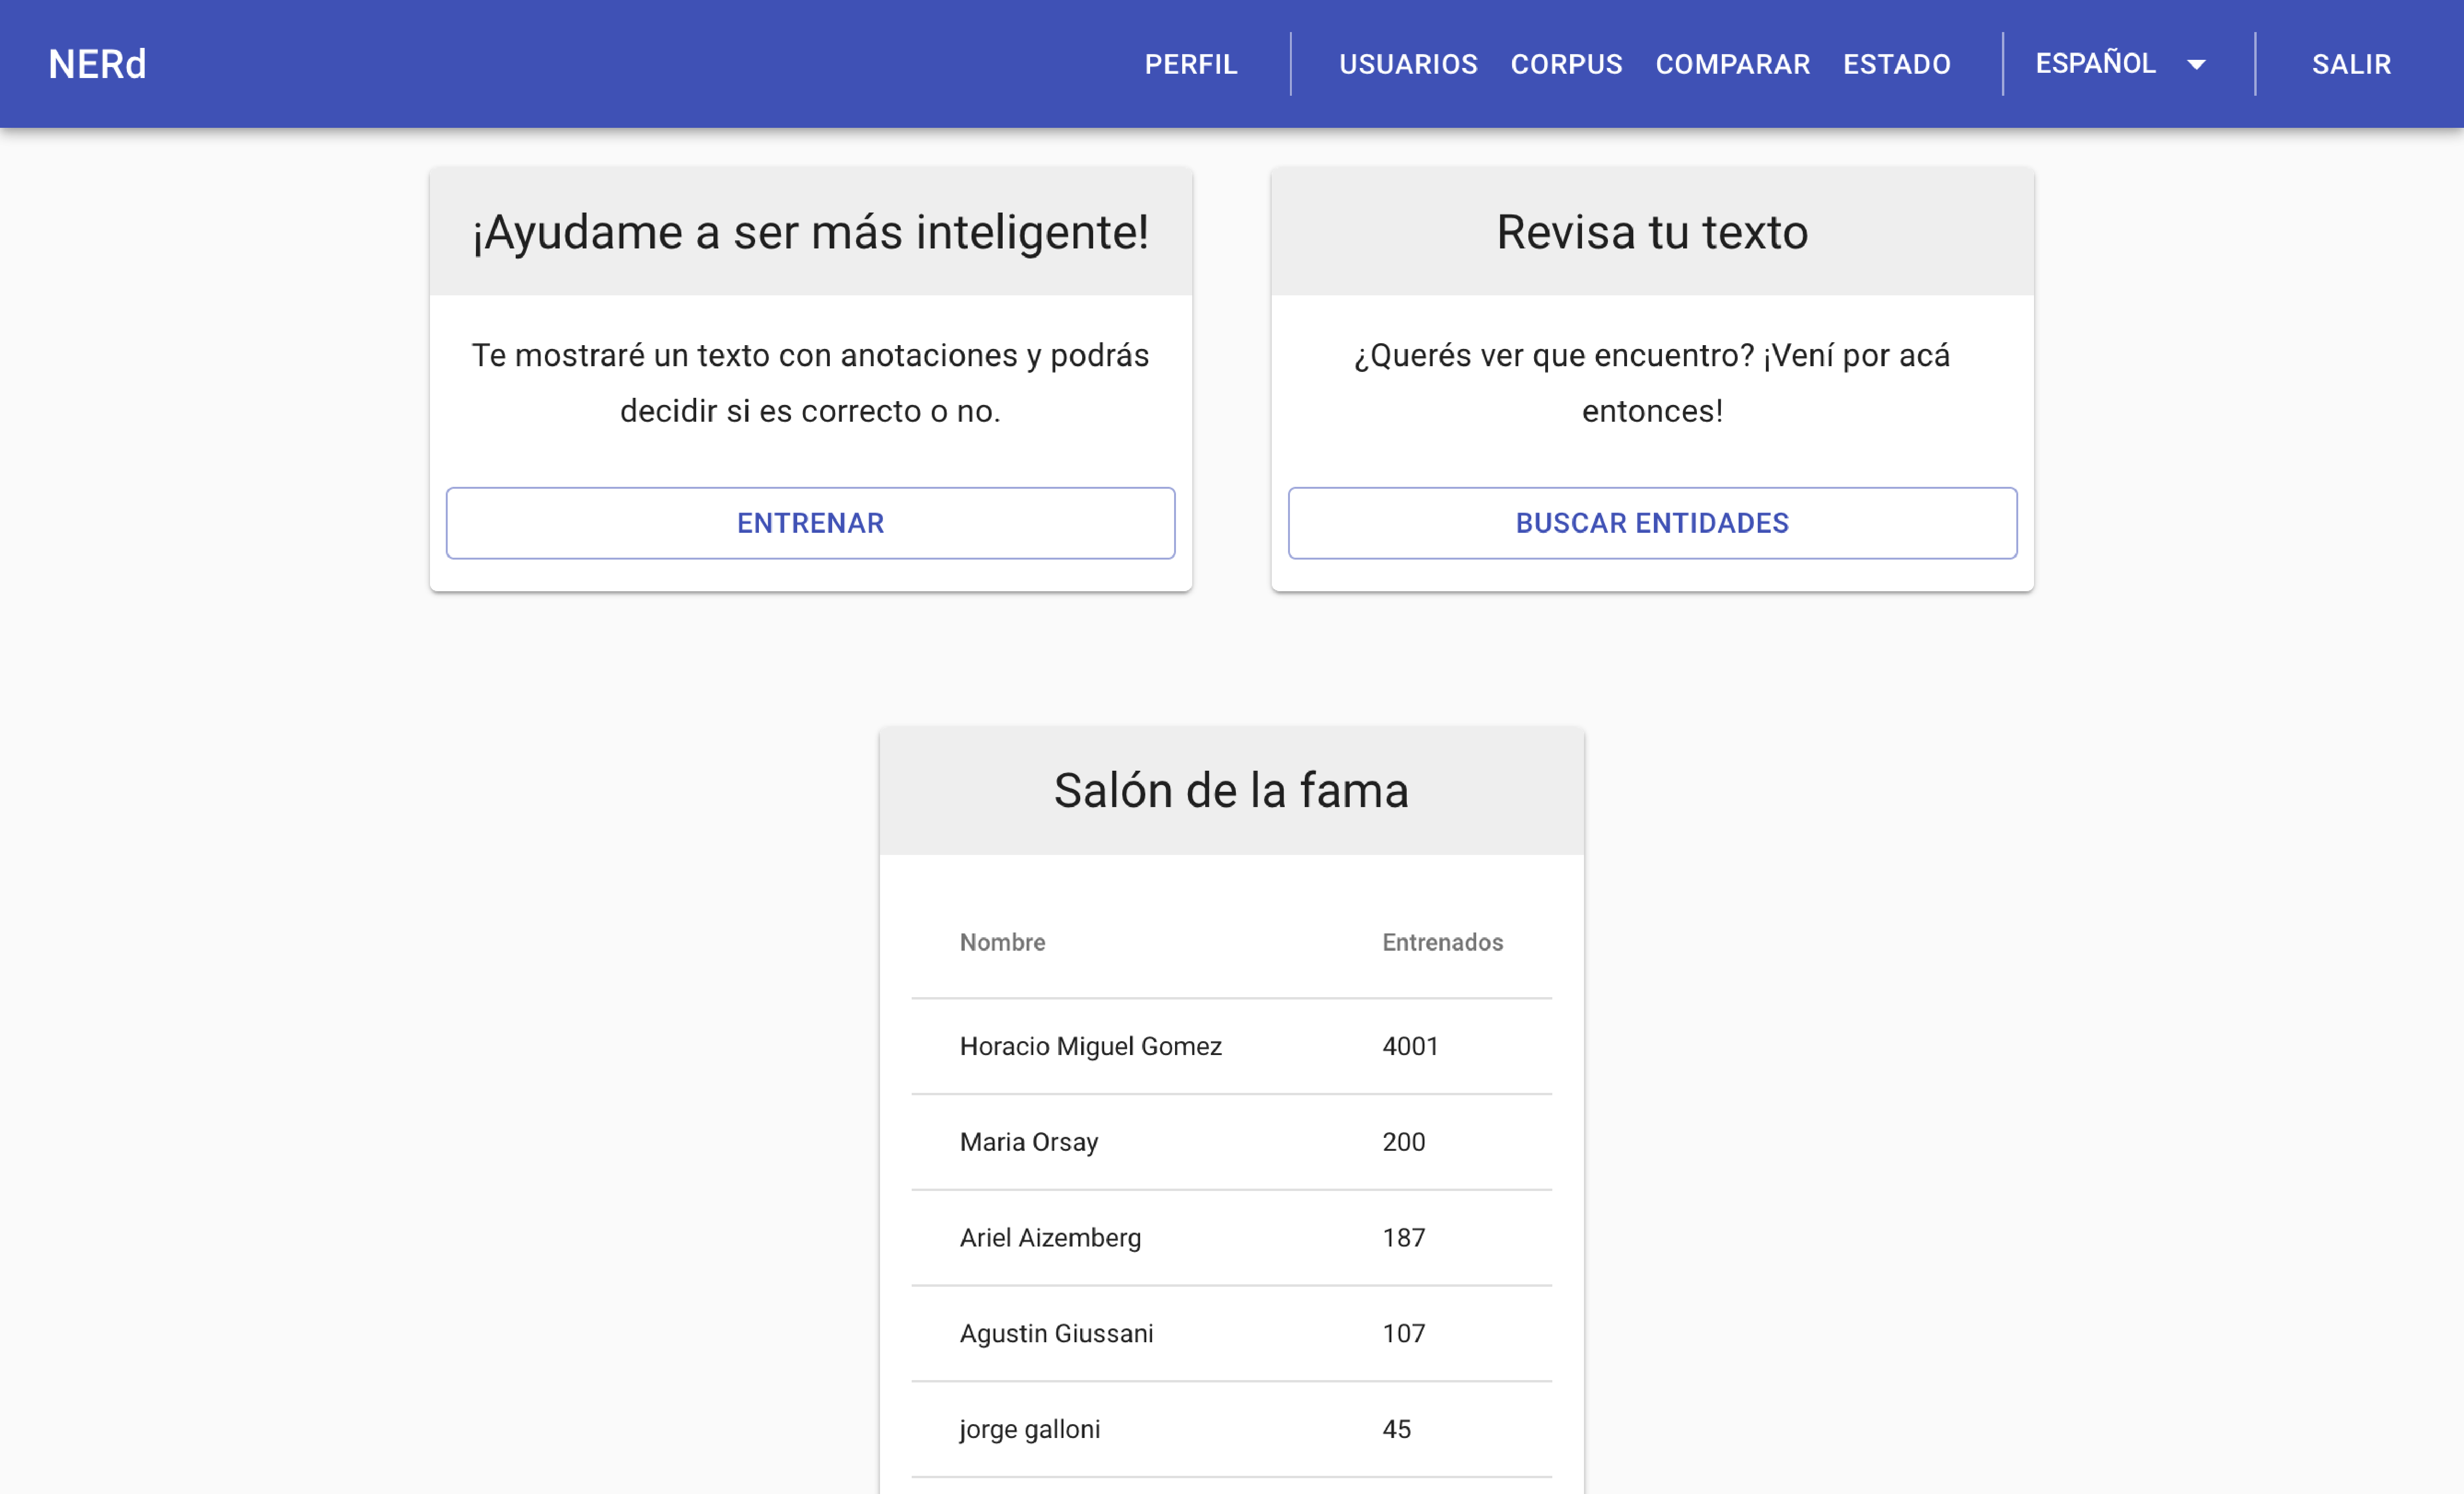
\includegraphics{assets/logic/home-logged-all.pdf} 

}

\caption{Pantalla de inicio con usuario logueado}\label{fig:logic-home}
\end{figure}

Si la persona no cuenta con permisos de entrenador, se le sugiere que contacte a un administrador para que le otorgue el permiso.

\begin{figure}[H]

{\centering 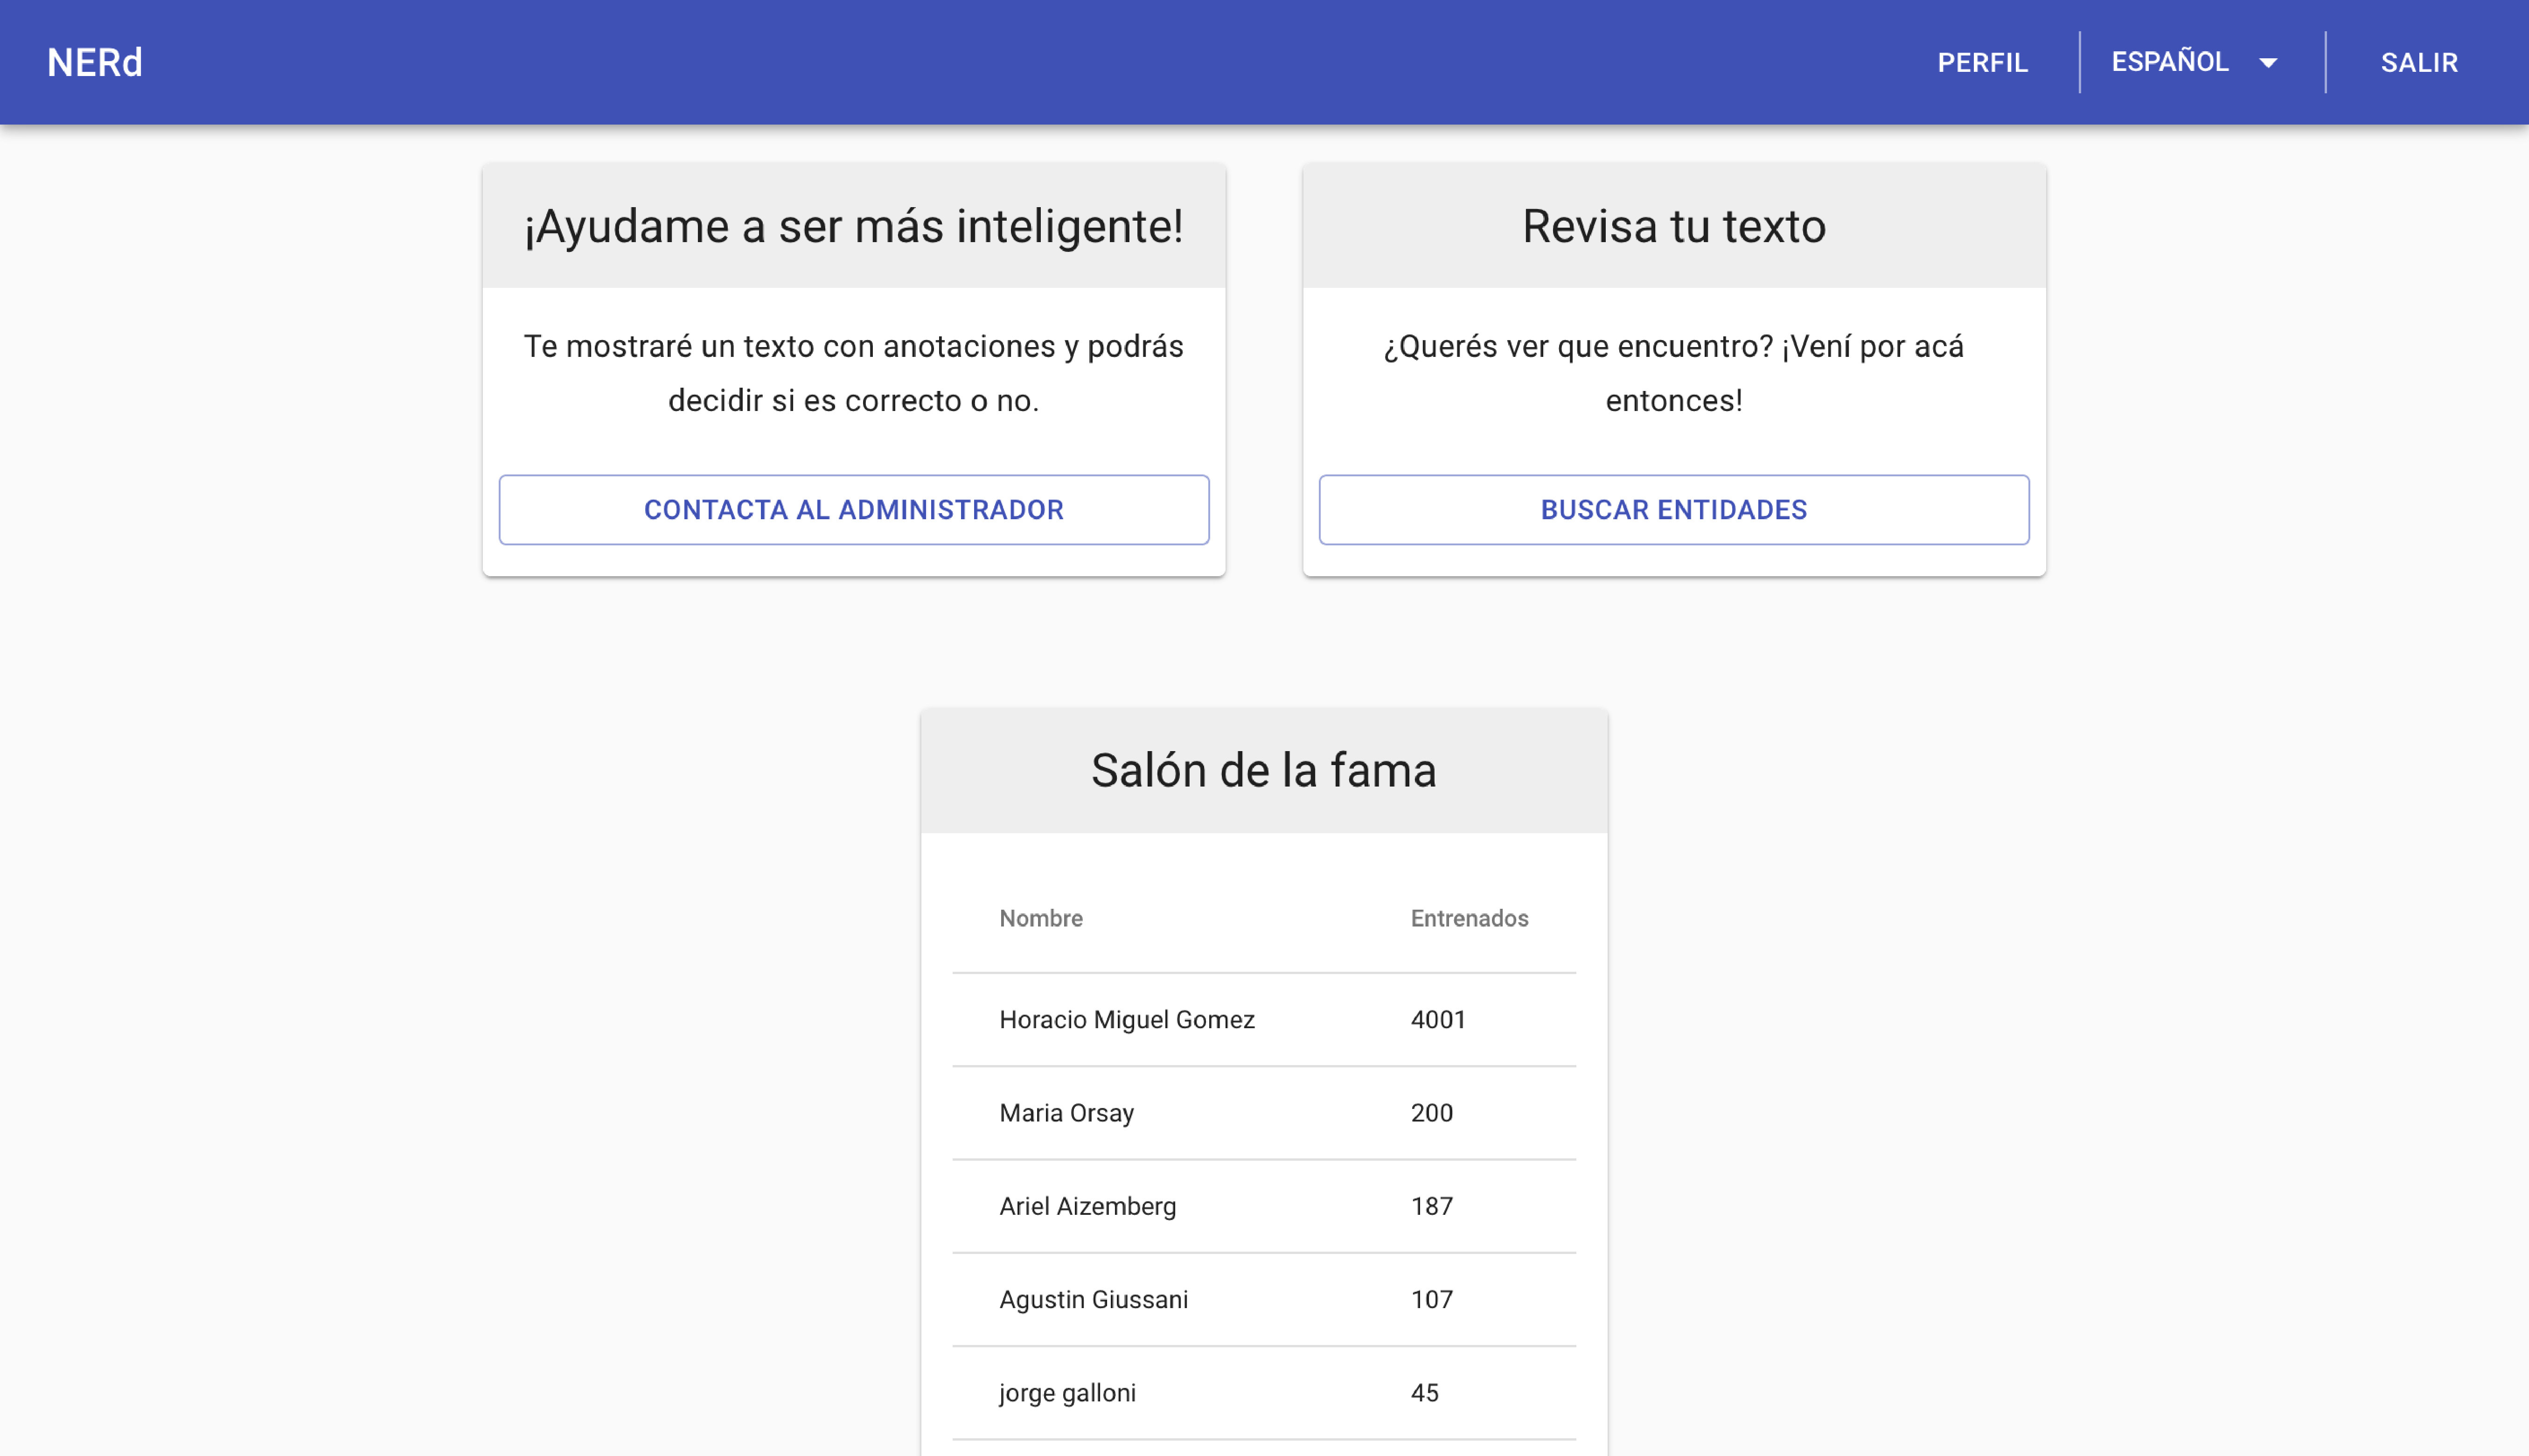
\includegraphics{assets/logic/home-logged-not_trainer.pdf} 

}

\caption{Pantalla de inicio sin rol de entrenador}\label{fig:logic-home-logged-nontrainer}
\end{figure}

Si la persona visitando la página no cuenta con una sesión activa, se le invita a ingresar con una cuenta pre-existente o a registrarse.

\begin{figure}[H]

{\centering 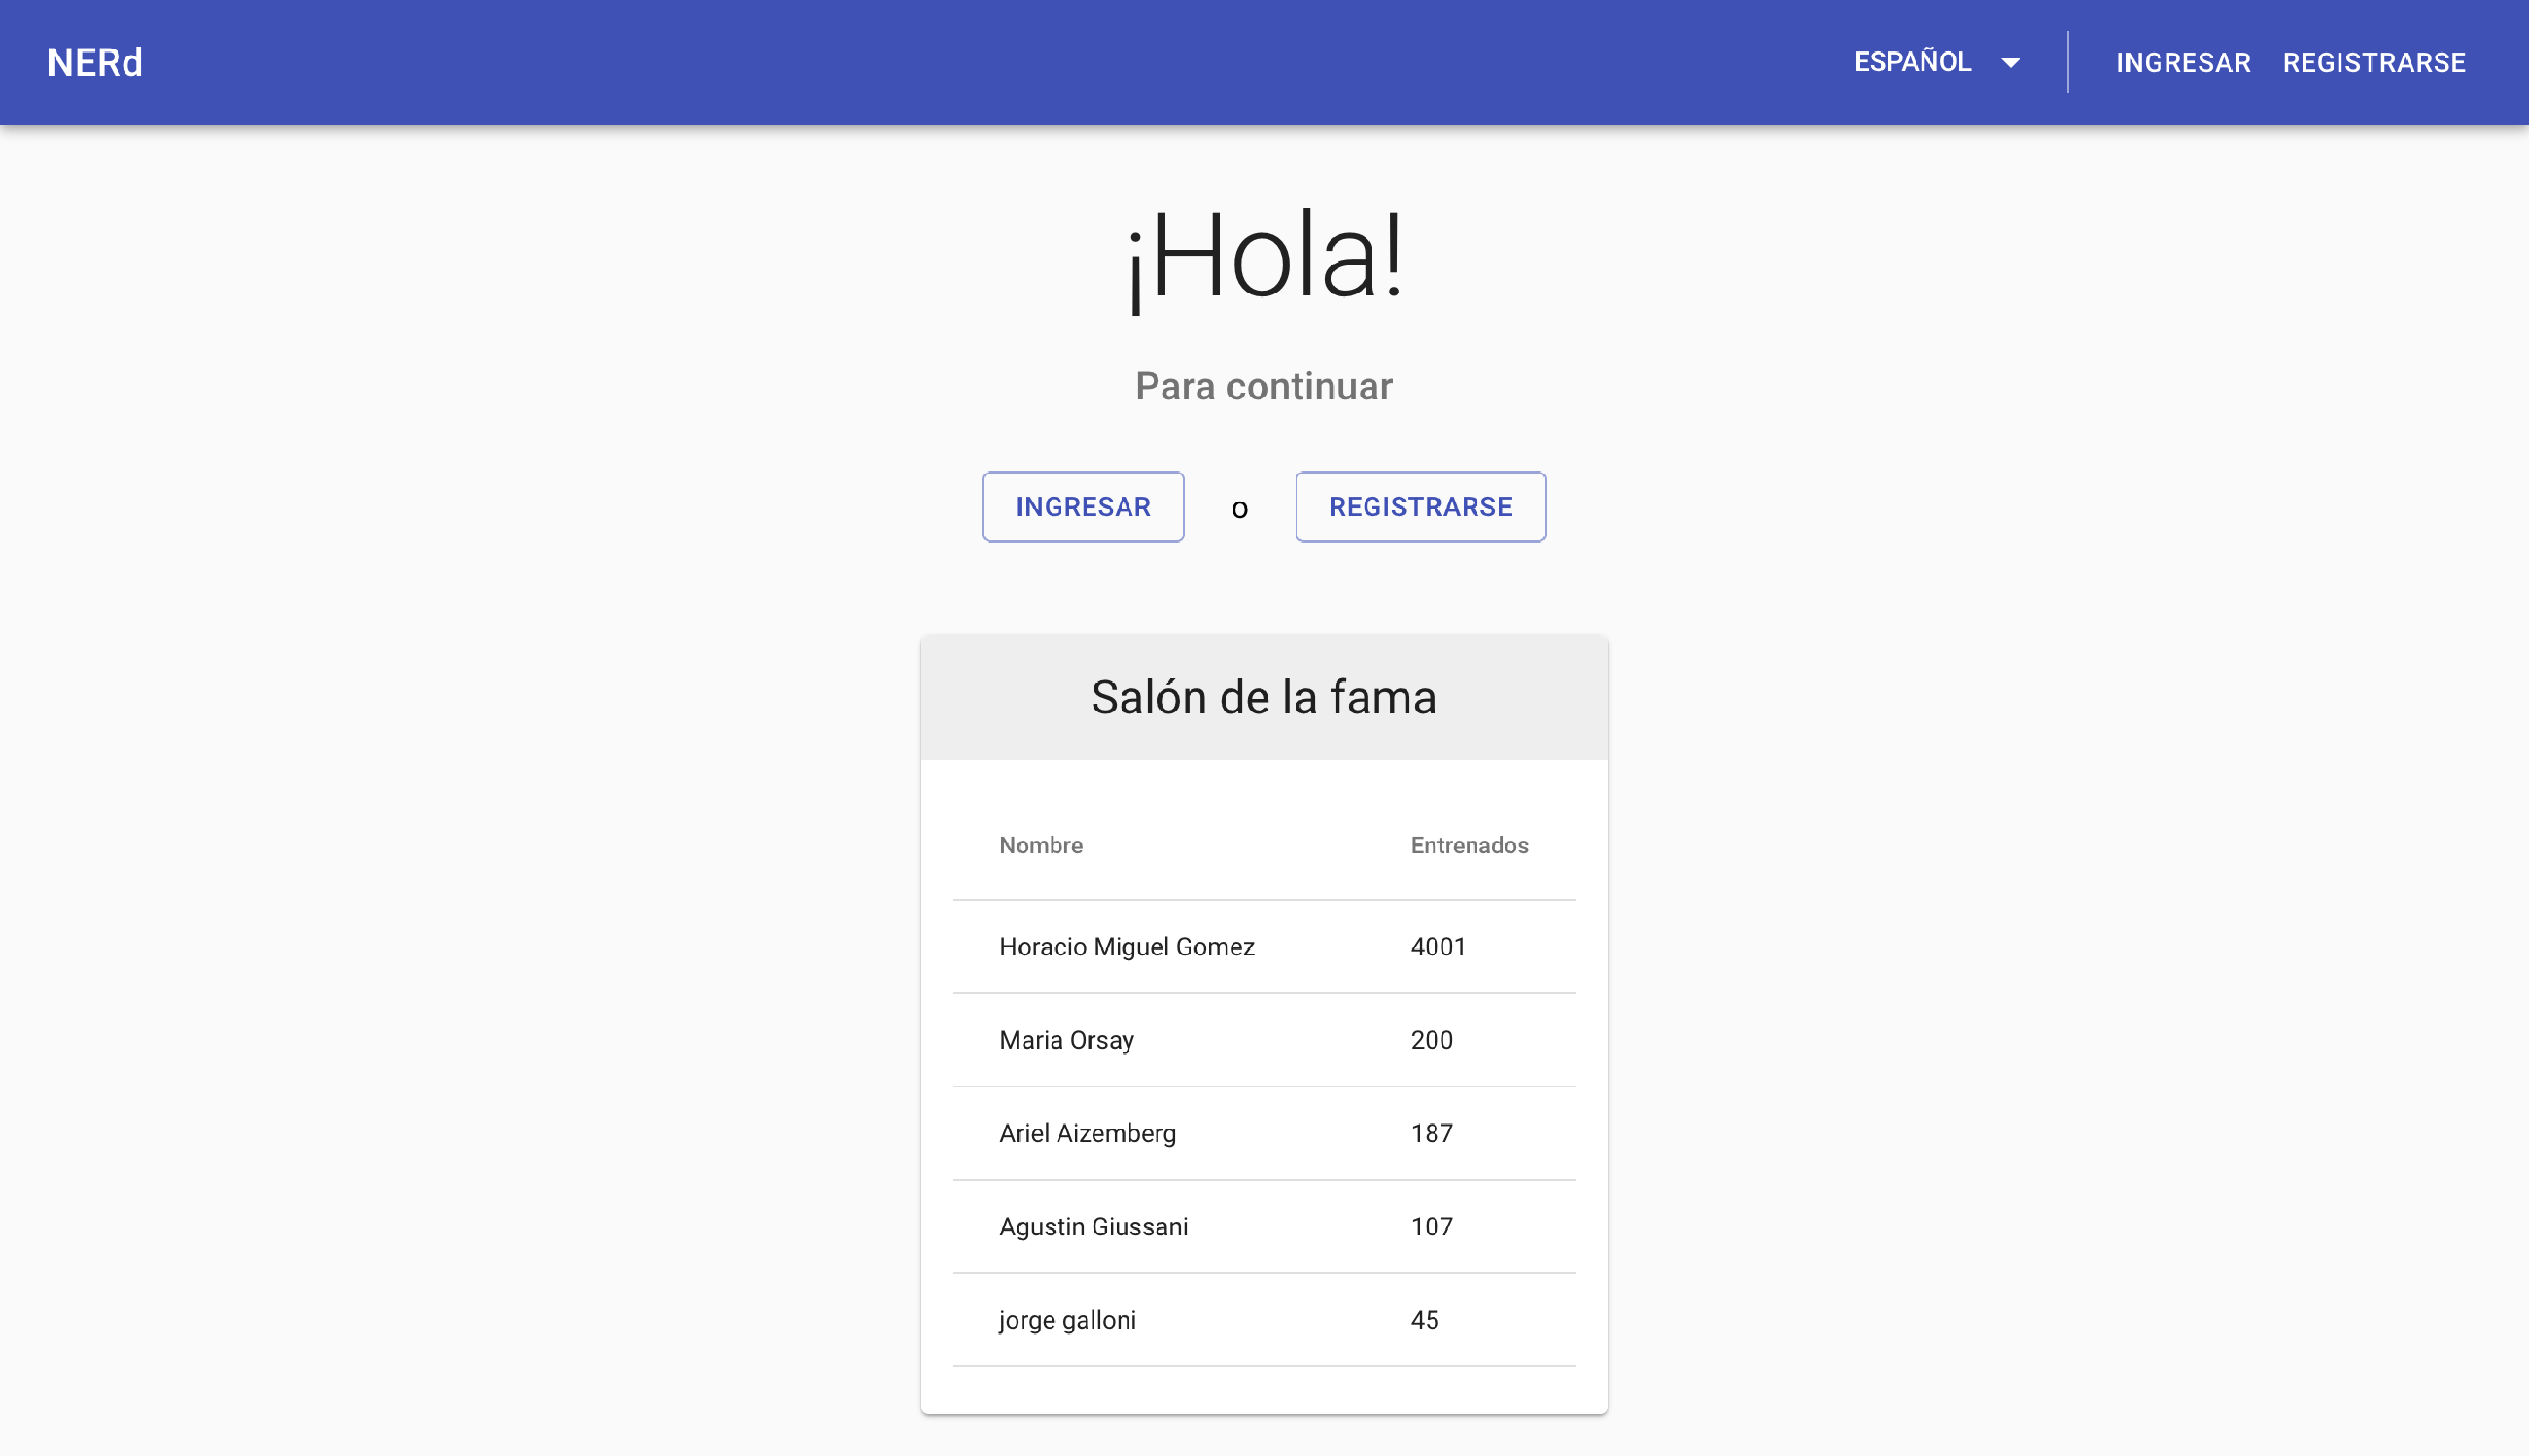
\includegraphics{assets/logic/home-anonymous.pdf} 

}

\caption{Pantalla de inicio sin sesión}\label{fig:logic-home-anonymous}
\end{figure}

\hypertarget{entrenamiento}{%
\paragraph{Entrenamiento}\label{entrenamiento}}

La pantalla de \emph{Entrenamiento} es el núcleo de la web en la cual es posible entrenar el modelo.

El usuario es presentado con un texto perteneciente al Corpus del servicio con las entidades inferidas por el modelo actual. Con un editor especial, le permitimos al usuario poder corregir las entidades inferidas y enviarle la corrección al servicio. Esa corrección será utilizada posteriormente a la hora de mejorar el modelo actual.

\begin{figure}[H]

{\centering 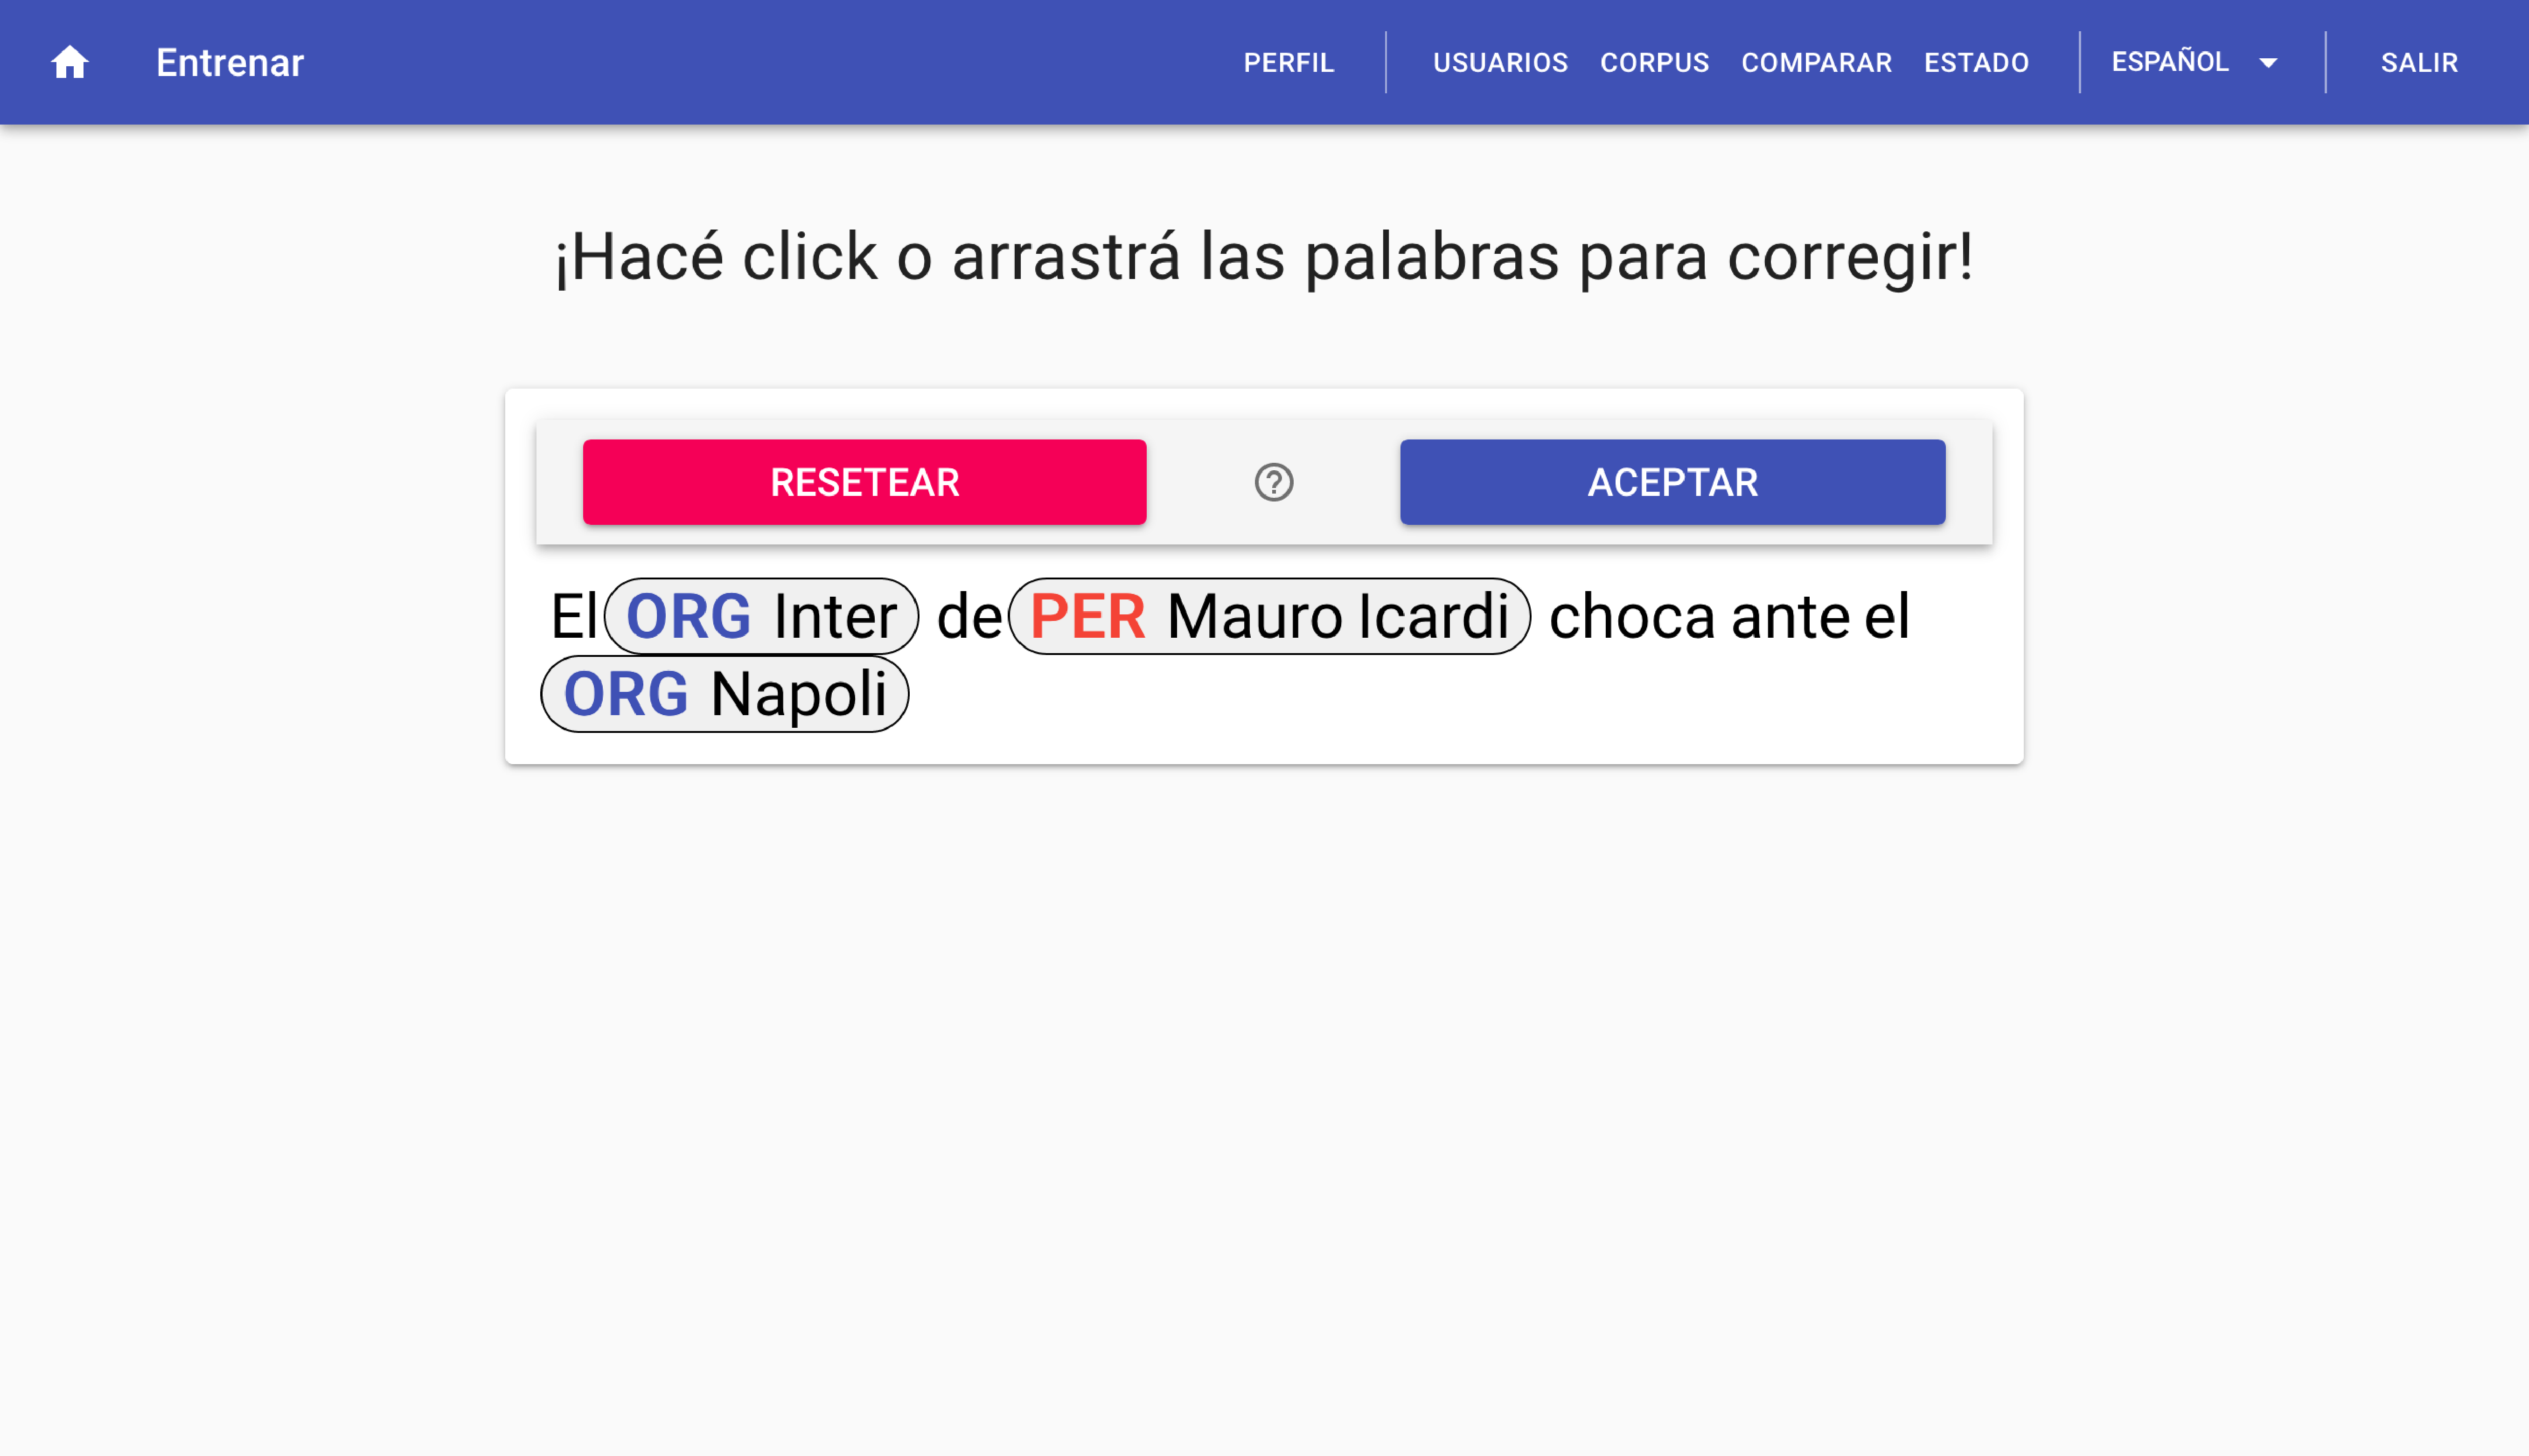
\includegraphics{assets/logic/train.pdf} 

}

\caption{Pantalla de entrenamiento}\label{fig:logic-train}
\end{figure}

\hypertarget{usabilidad}{%
\subparagraph{Usabilidad}\label{usabilidad}}

Tuvimos un foco fuerte en la usabilidad del widget ya que los entrenadores del servicio van a pasar prácticamente todo su tiempo en ésta pantalla, por lo que se tuvieron las siguientes consideraciones en la implementación.

Llamado a acción y ayuda

Dado que lo primero que ve el usuario es un texto con anotaciones, agregamos un título que invita al usuario a realizar acciones sobre el texto. De esta manera, le mostramos las dos acciones principales realizables desde el widget de entrenamiento: Click en alguna palabra o entidad y arrastrar un conjunto de palabras para crear una entidad nueva.
Como refuerzo de este llamado a acción, agregamos un botón que al ser clickeado muestra un mensaje de ayuda con instrucciones más detalladas sobre el objetivo del entrenador y las acciones que deben de realizarse sobre el mismo.

\begin{figure}[H]

{\centering 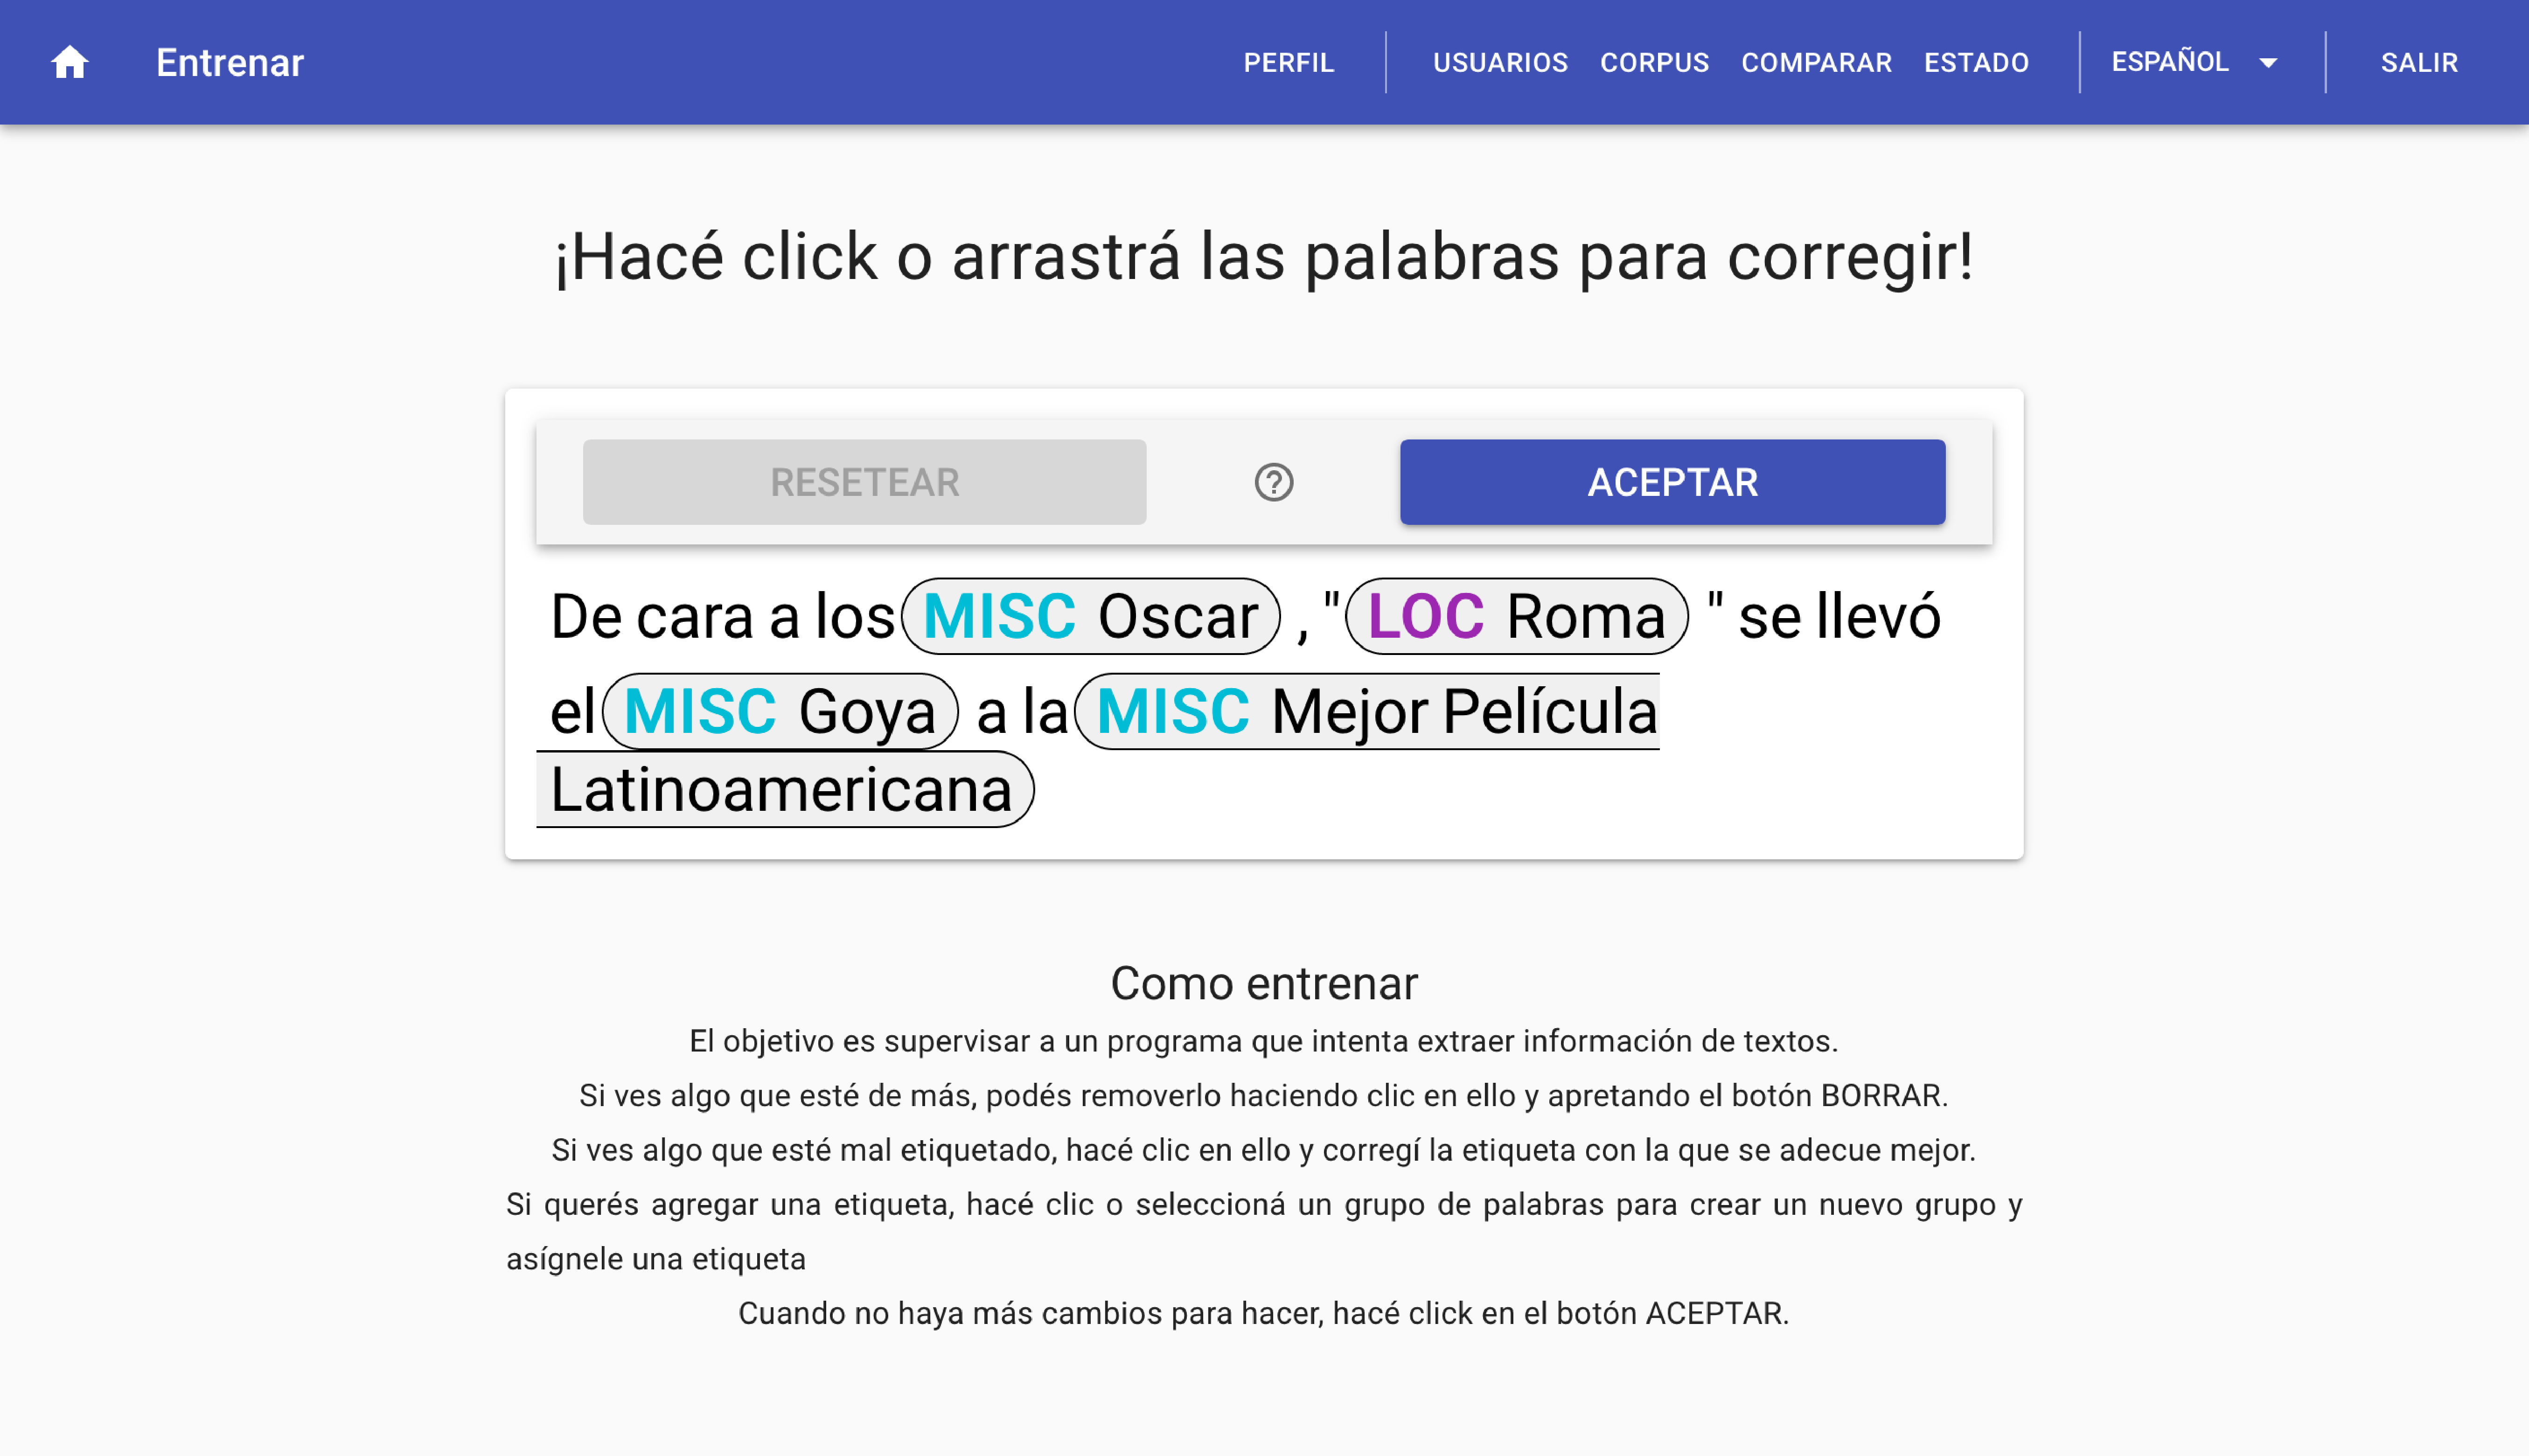
\includegraphics{assets/logic/train-help.pdf} 

}

\caption{Ayuda del entrenador}\label{fig:logic-train-help}
\end{figure}

Creación y edición de entidades

Para la creación de entidades decidimos ofrecer dos maneras: La primera es arrastrando un conjunto de palabras de manera tal de unirlas todas en una única entidad.
La otra es hacer click en una palabra y ahí se ofrecen opciones dependiendo de la ubicación de la palabra dentro del texto:

\begin{itemize}
\tightlist
\item
  Si no existen entidades en el texto actual, se le asigna por defecto el tipo \emph{MISC} y se muestran el resto de los tipos para permitir cambiarlo de ser necesario.
\item
  Si existen entidades antes o después, se ofrece la opción de unir la palabra actual con la entidada más próxima para el lado elegido.
\end{itemize}

\begin{figure}[H]

{\centering 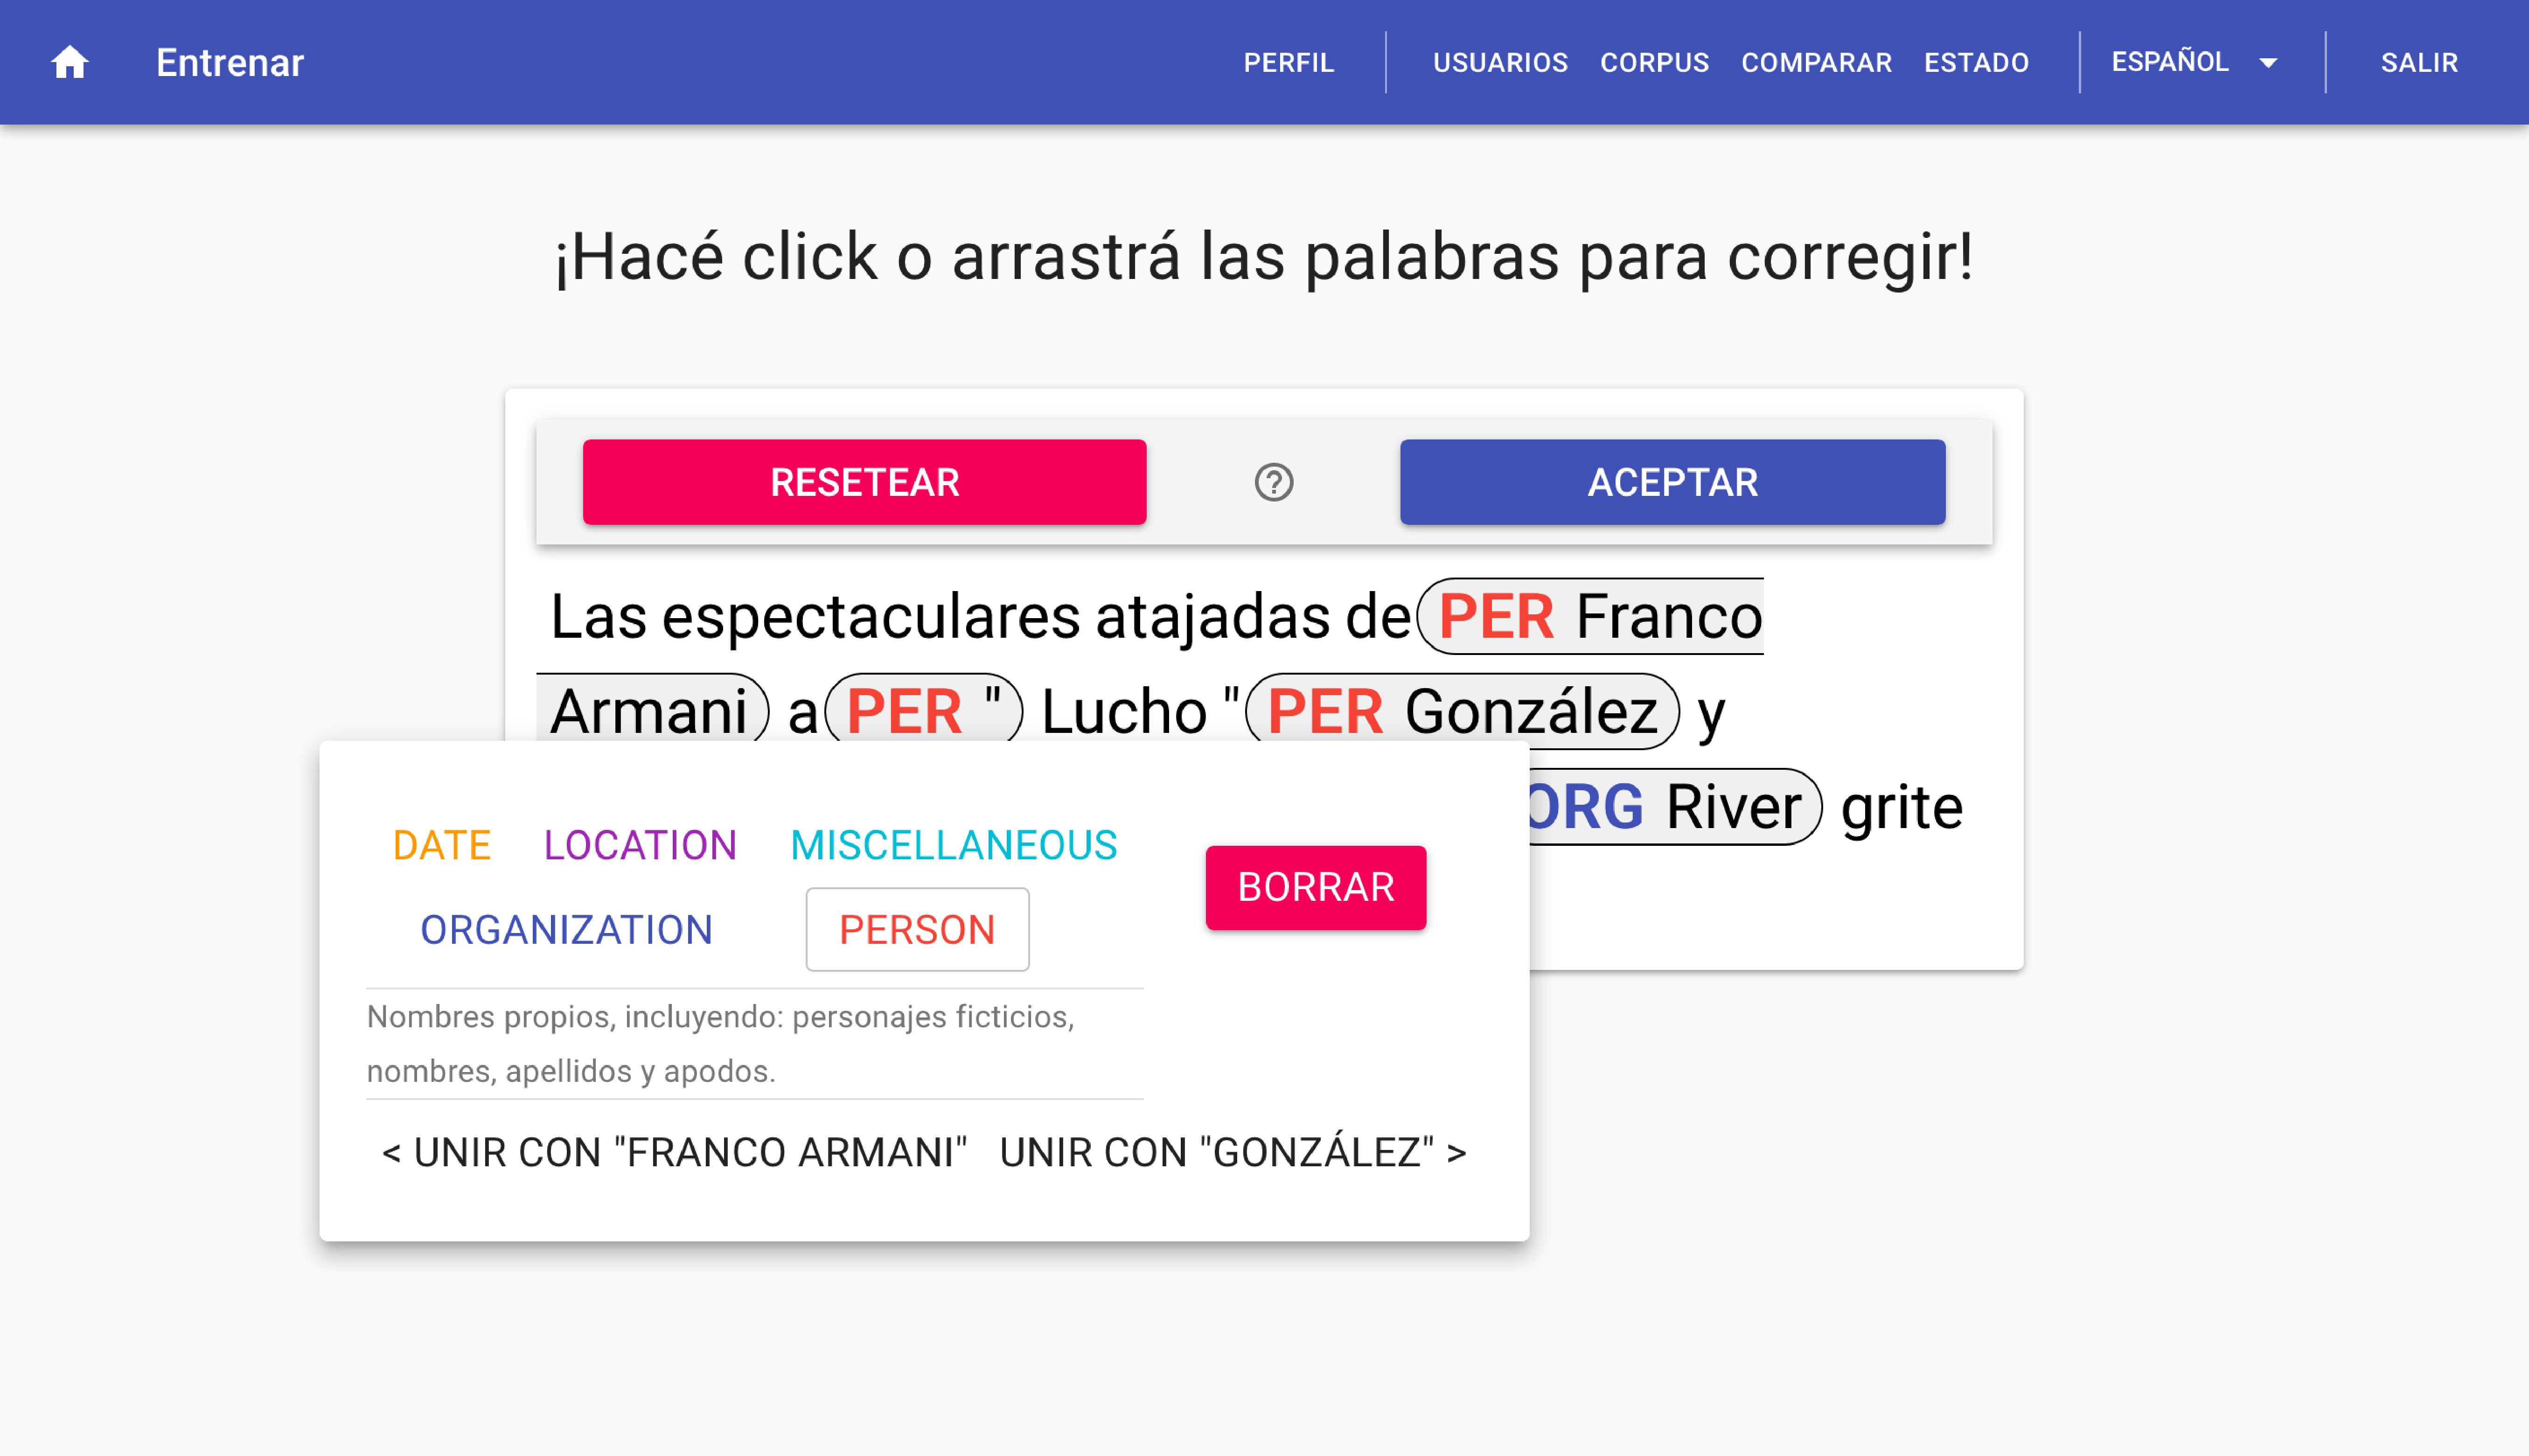
\includegraphics{assets/logic/train-popup.pdf} 

}

\caption{Edición de entidad}\label{fig:logic-train-popup}
\end{figure}

Para la edición de entidades decidimos permitir únicamente la modificación del tipo de una entidad inferida.
Si el modelo infirió una entidad de manera incorrecta, ya sea por que sea una entidad inválida o agregó palabras de más a una entidad inválida, permitimos que el usuario remueva la entidad y que después vuelva a agregar la entidad correcta.

Optimización en tiempos de carga

Dado que es esperado que un usuario entrene más de un texto, al momento de pedir un texto para mostrar, se pide el siguiente. Mediante este mecanismo de pre-carga, podemos eliminar el tiempo de espera entre texto y texto ofreciendo al usuario una experiencia completamente fluida.

\hypertarget{administraciuxf3n-de-usuarios}{%
\paragraph{Administración de usuarios}\label{administraciuxf3n-de-usuarios}}

La pantalla de \emph{Administración de usuarios} permite a los usuarios con el rol de administrador poder modificar los roles de todos los usuarios del sistema, borrarlos o acceder a los detalles del usuario, tal como la lista de textos entrenados.

\begin{figure}[H]

{\centering 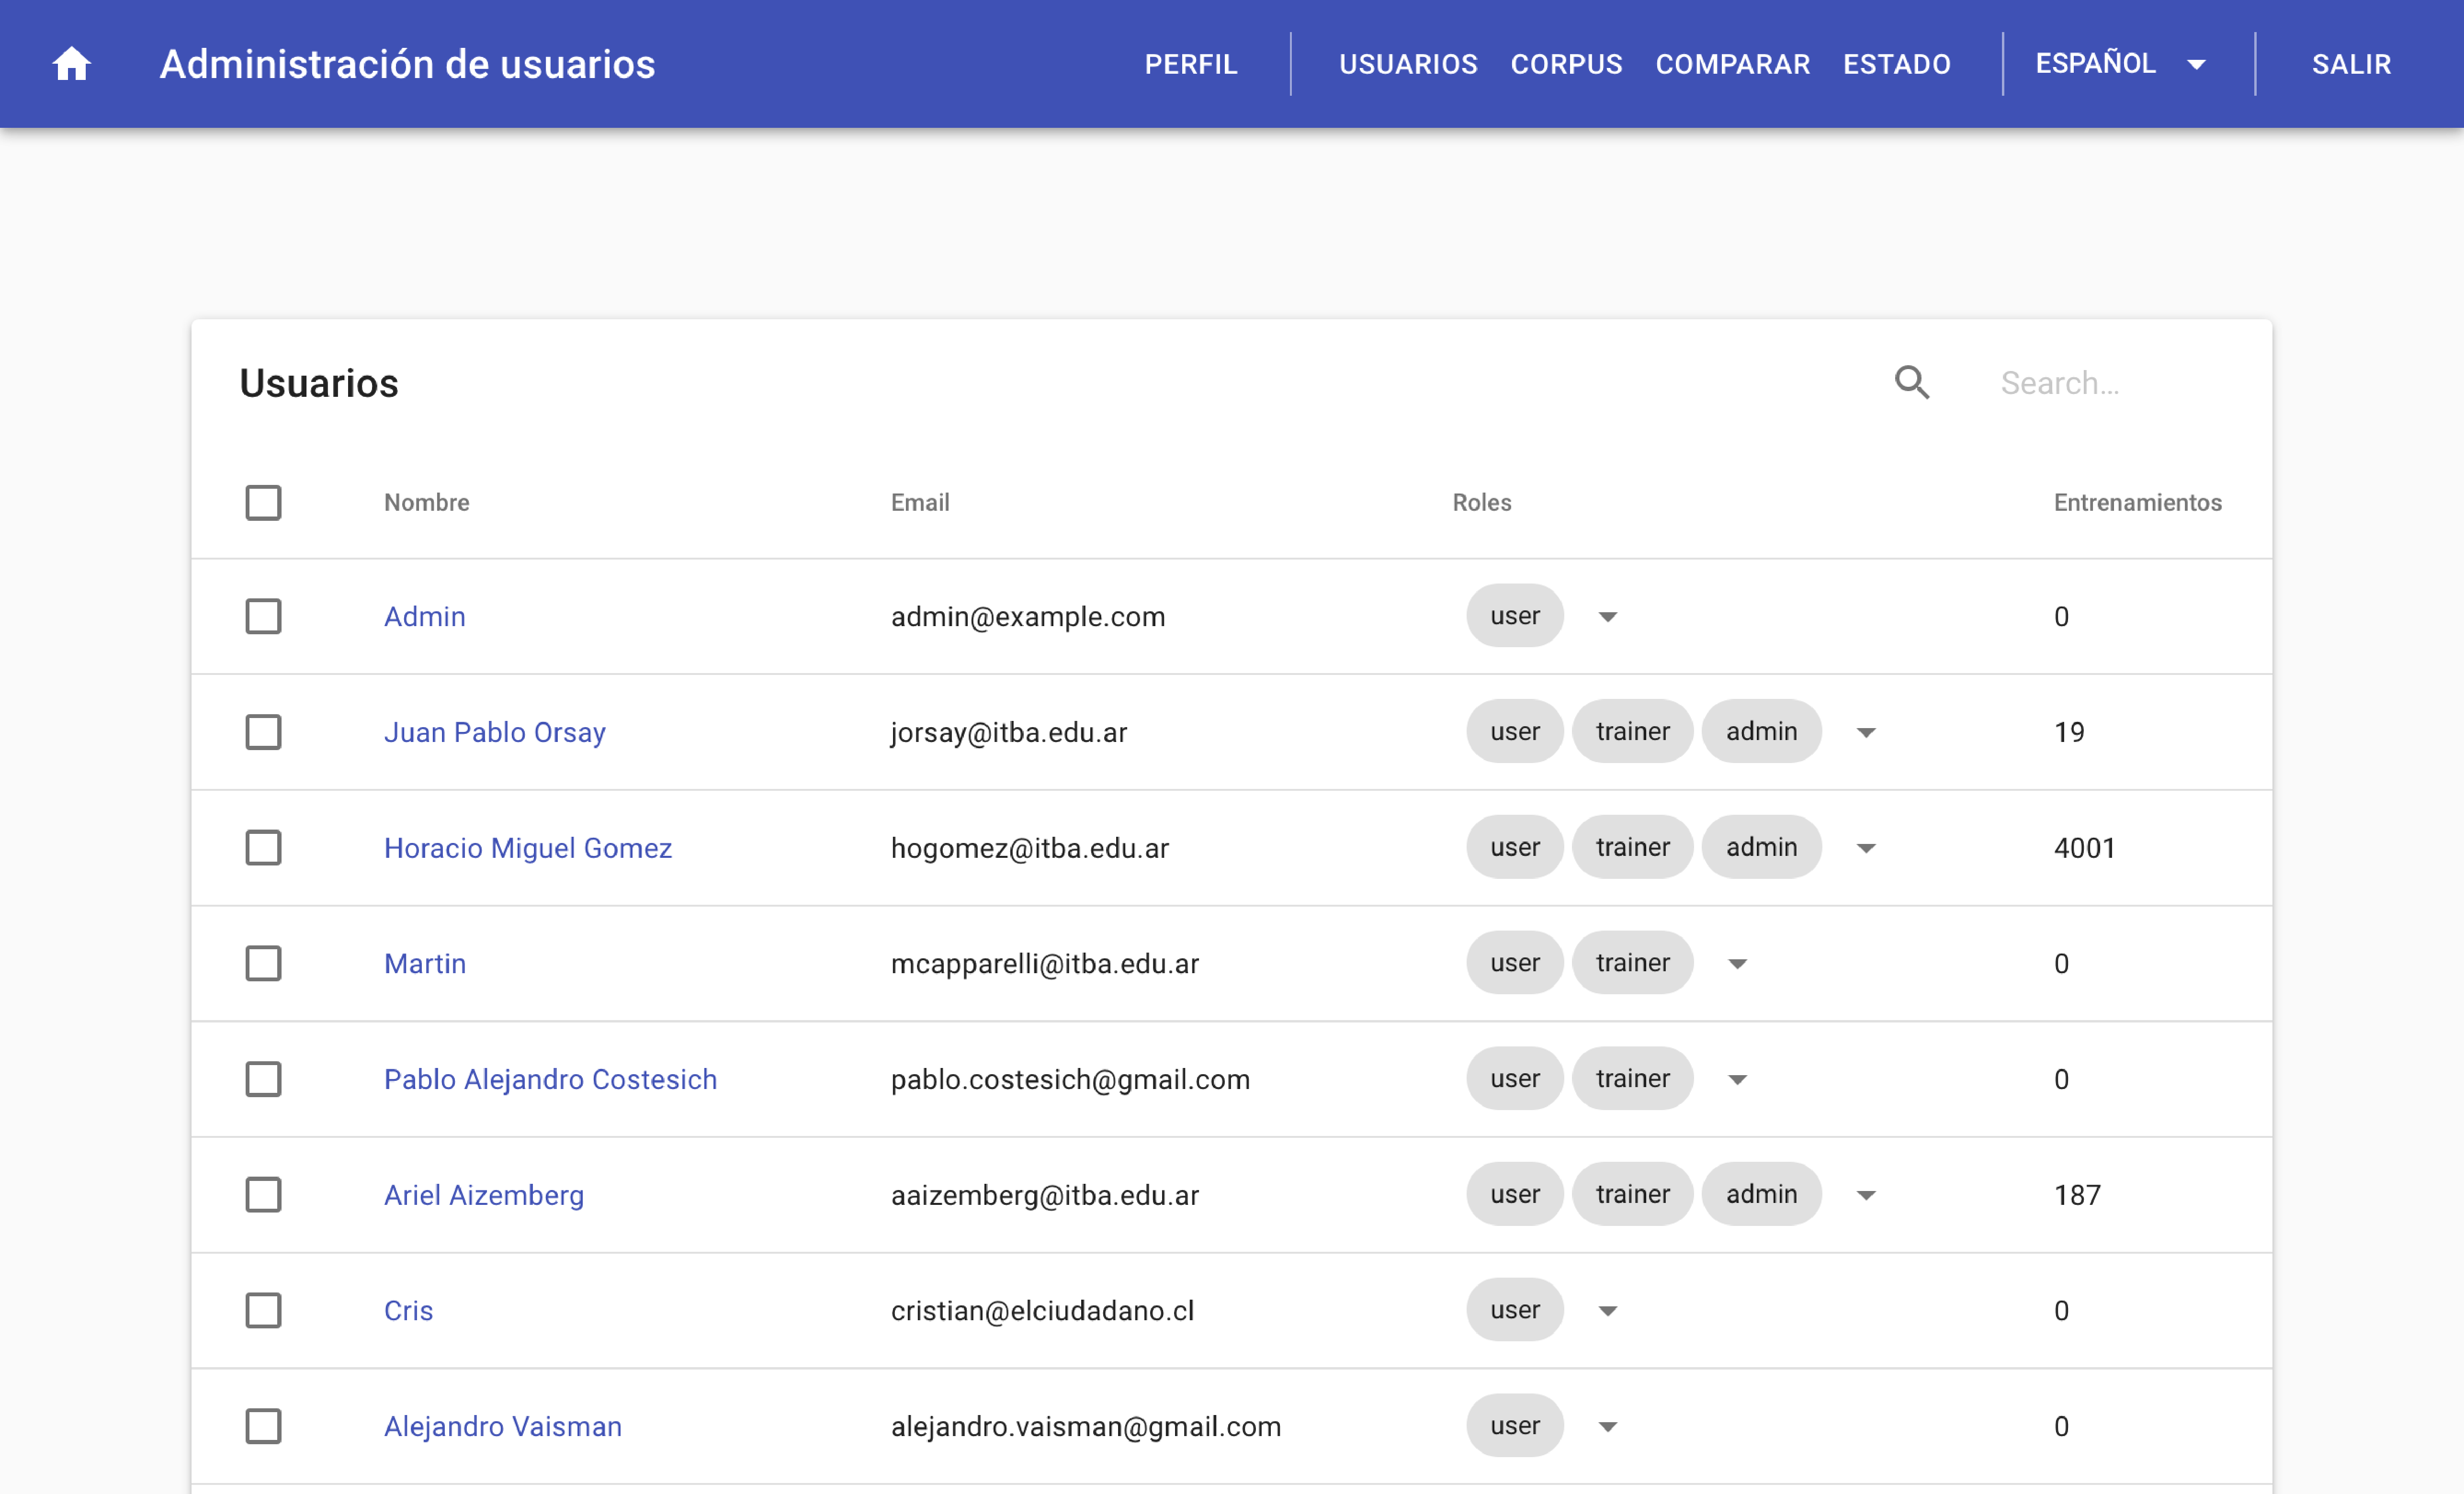
\includegraphics{assets/logic/user-list.pdf} 

}

\caption{Administración de usuarios}\label{fig:logic-user-list}
\end{figure}

\hypertarget{detalles-de-usuario}{%
\paragraph{Detalles de usuario}\label{detalles-de-usuario}}

La pantalla de detalle de usuario permite al usuario con sesión activa ver sus entrenamientos y cambiar su contraseña.

Los usuarios con rol administrador pueden realizar las acciones mencionadas previamente pero a otros usuarios.

\begin{figure}[H]

{\centering 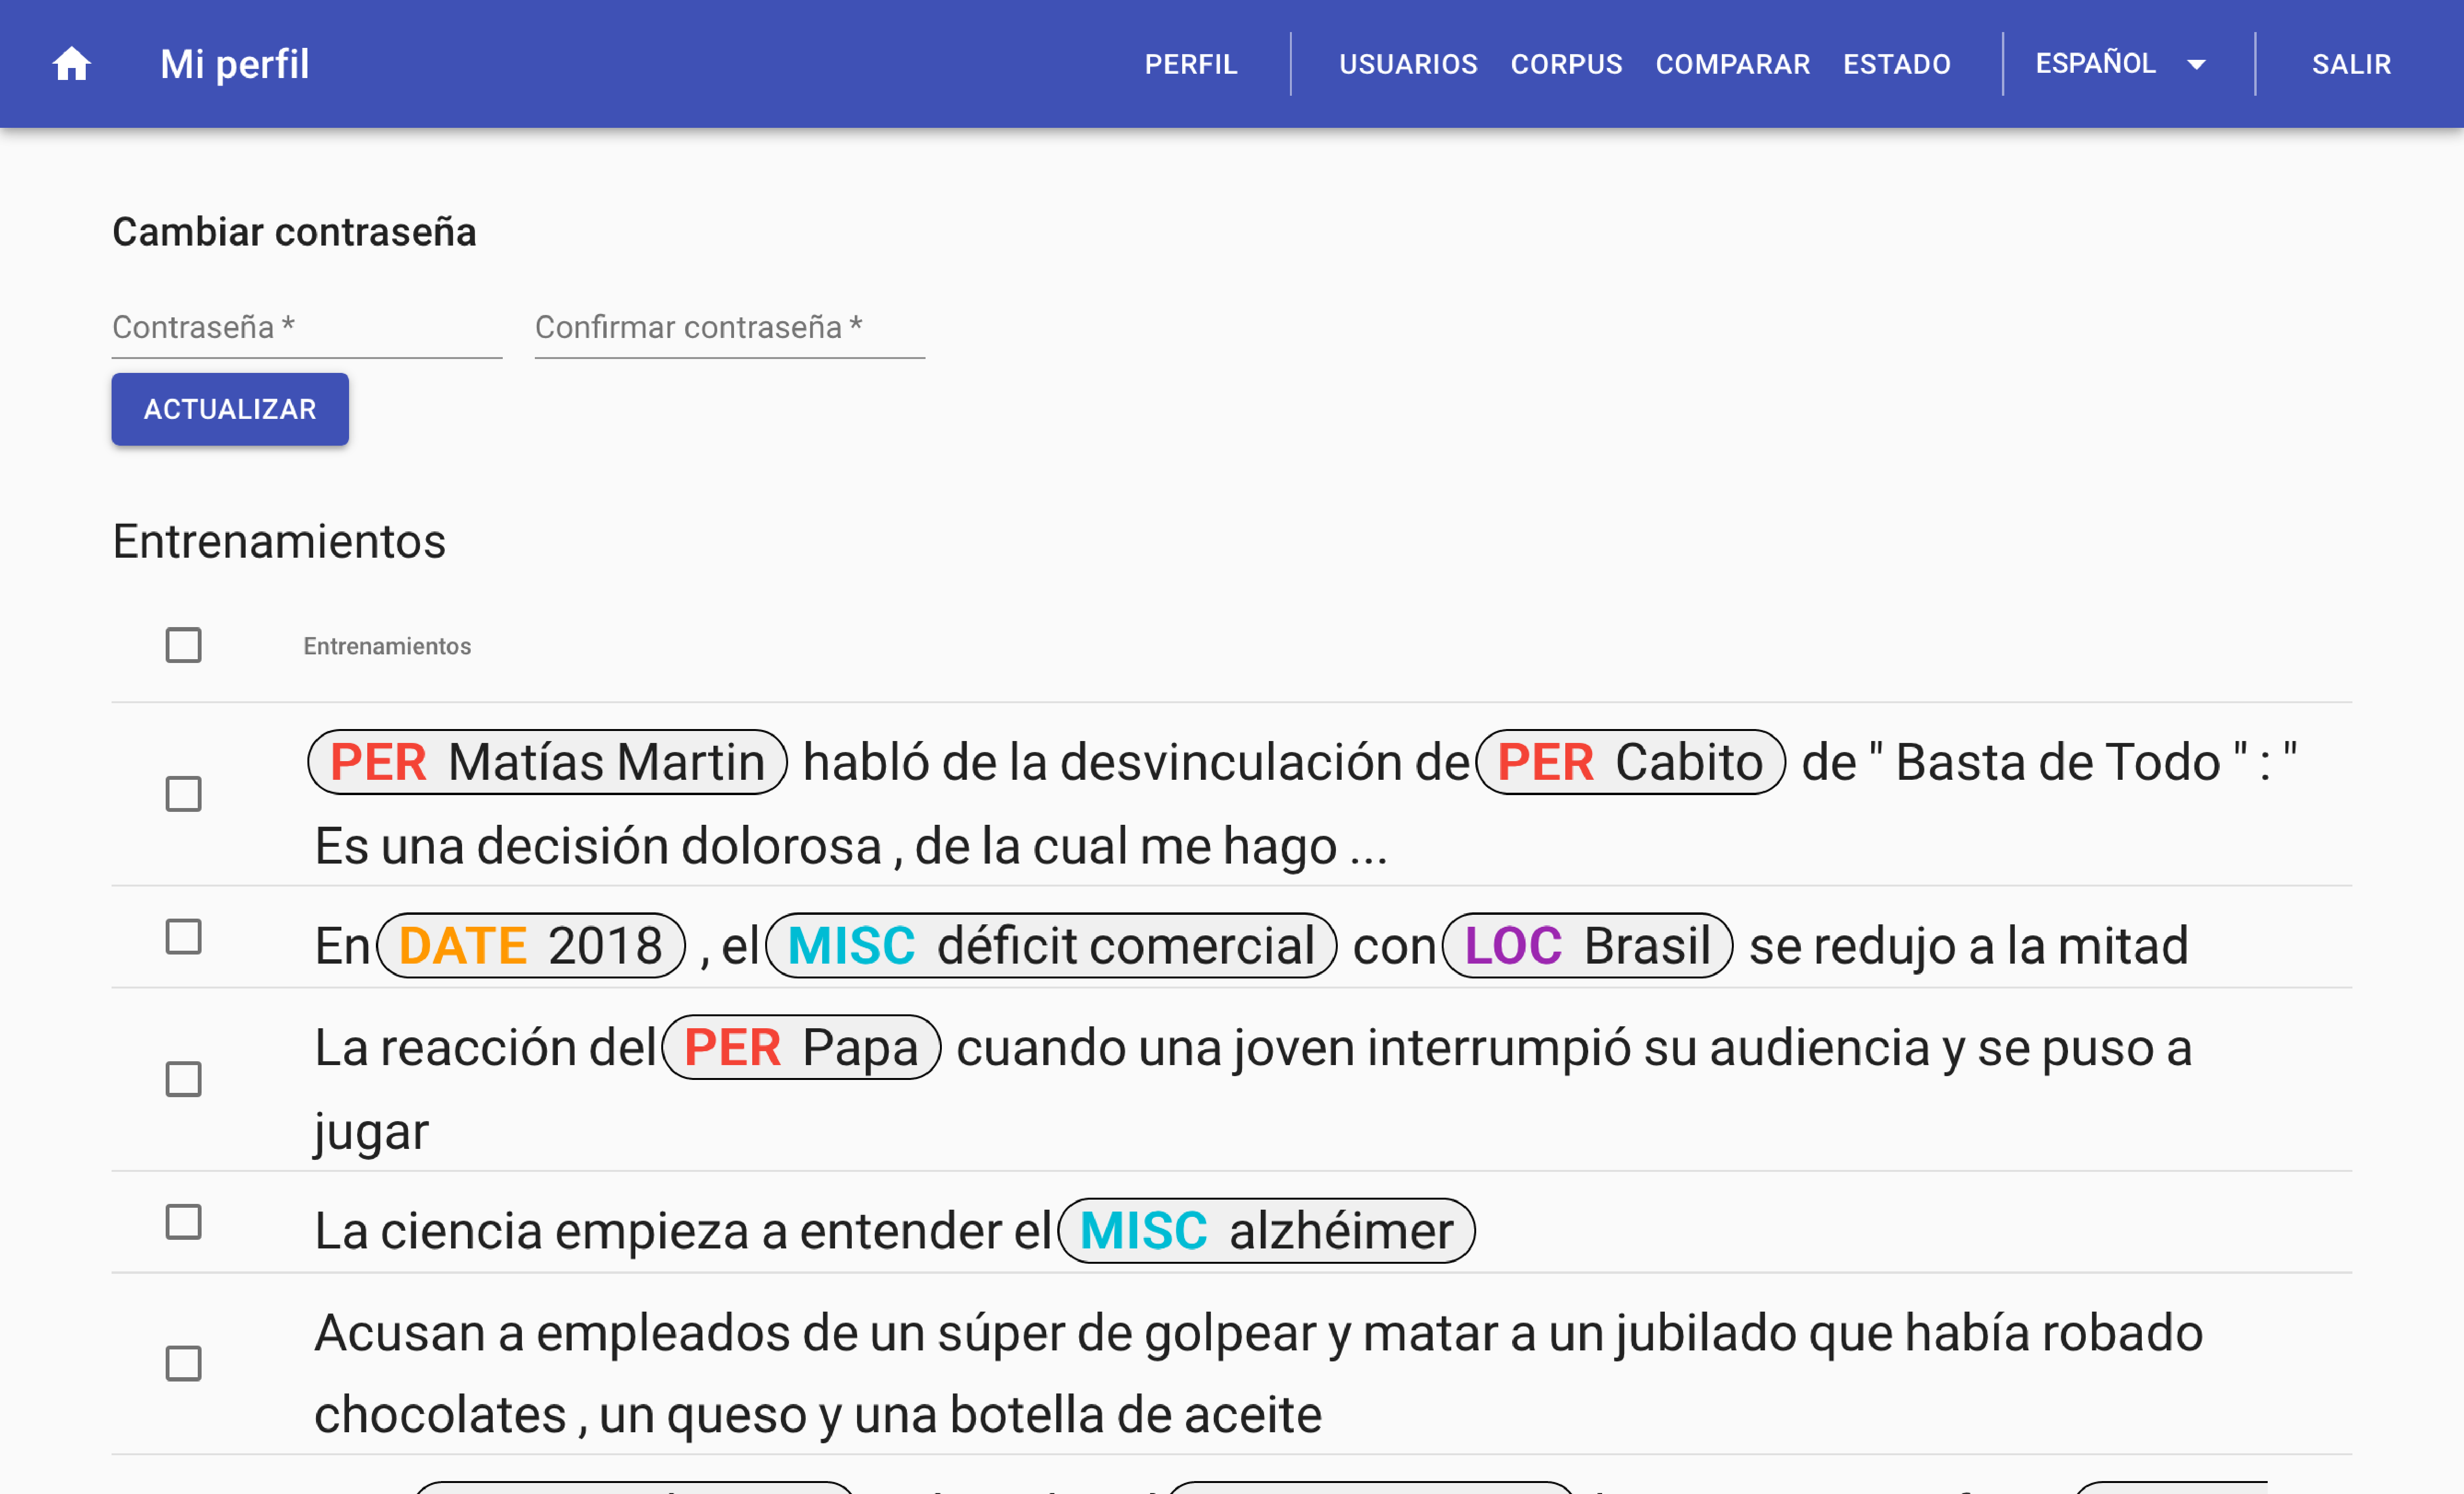
\includegraphics{assets/logic/user-profile.pdf} 

}

\caption{Perfil de usuario}\label{fig:logic-user-profile}
\end{figure}

\hypertarget{corpus-1}{%
\paragraph{Corpus}\label{corpus-1}}

La pantalla de \emph{Corpus} permite a un usuario con el rol de administrador realizar tareas relacionadas con el corpus del sistema.

\begin{figure}[H]

{\centering 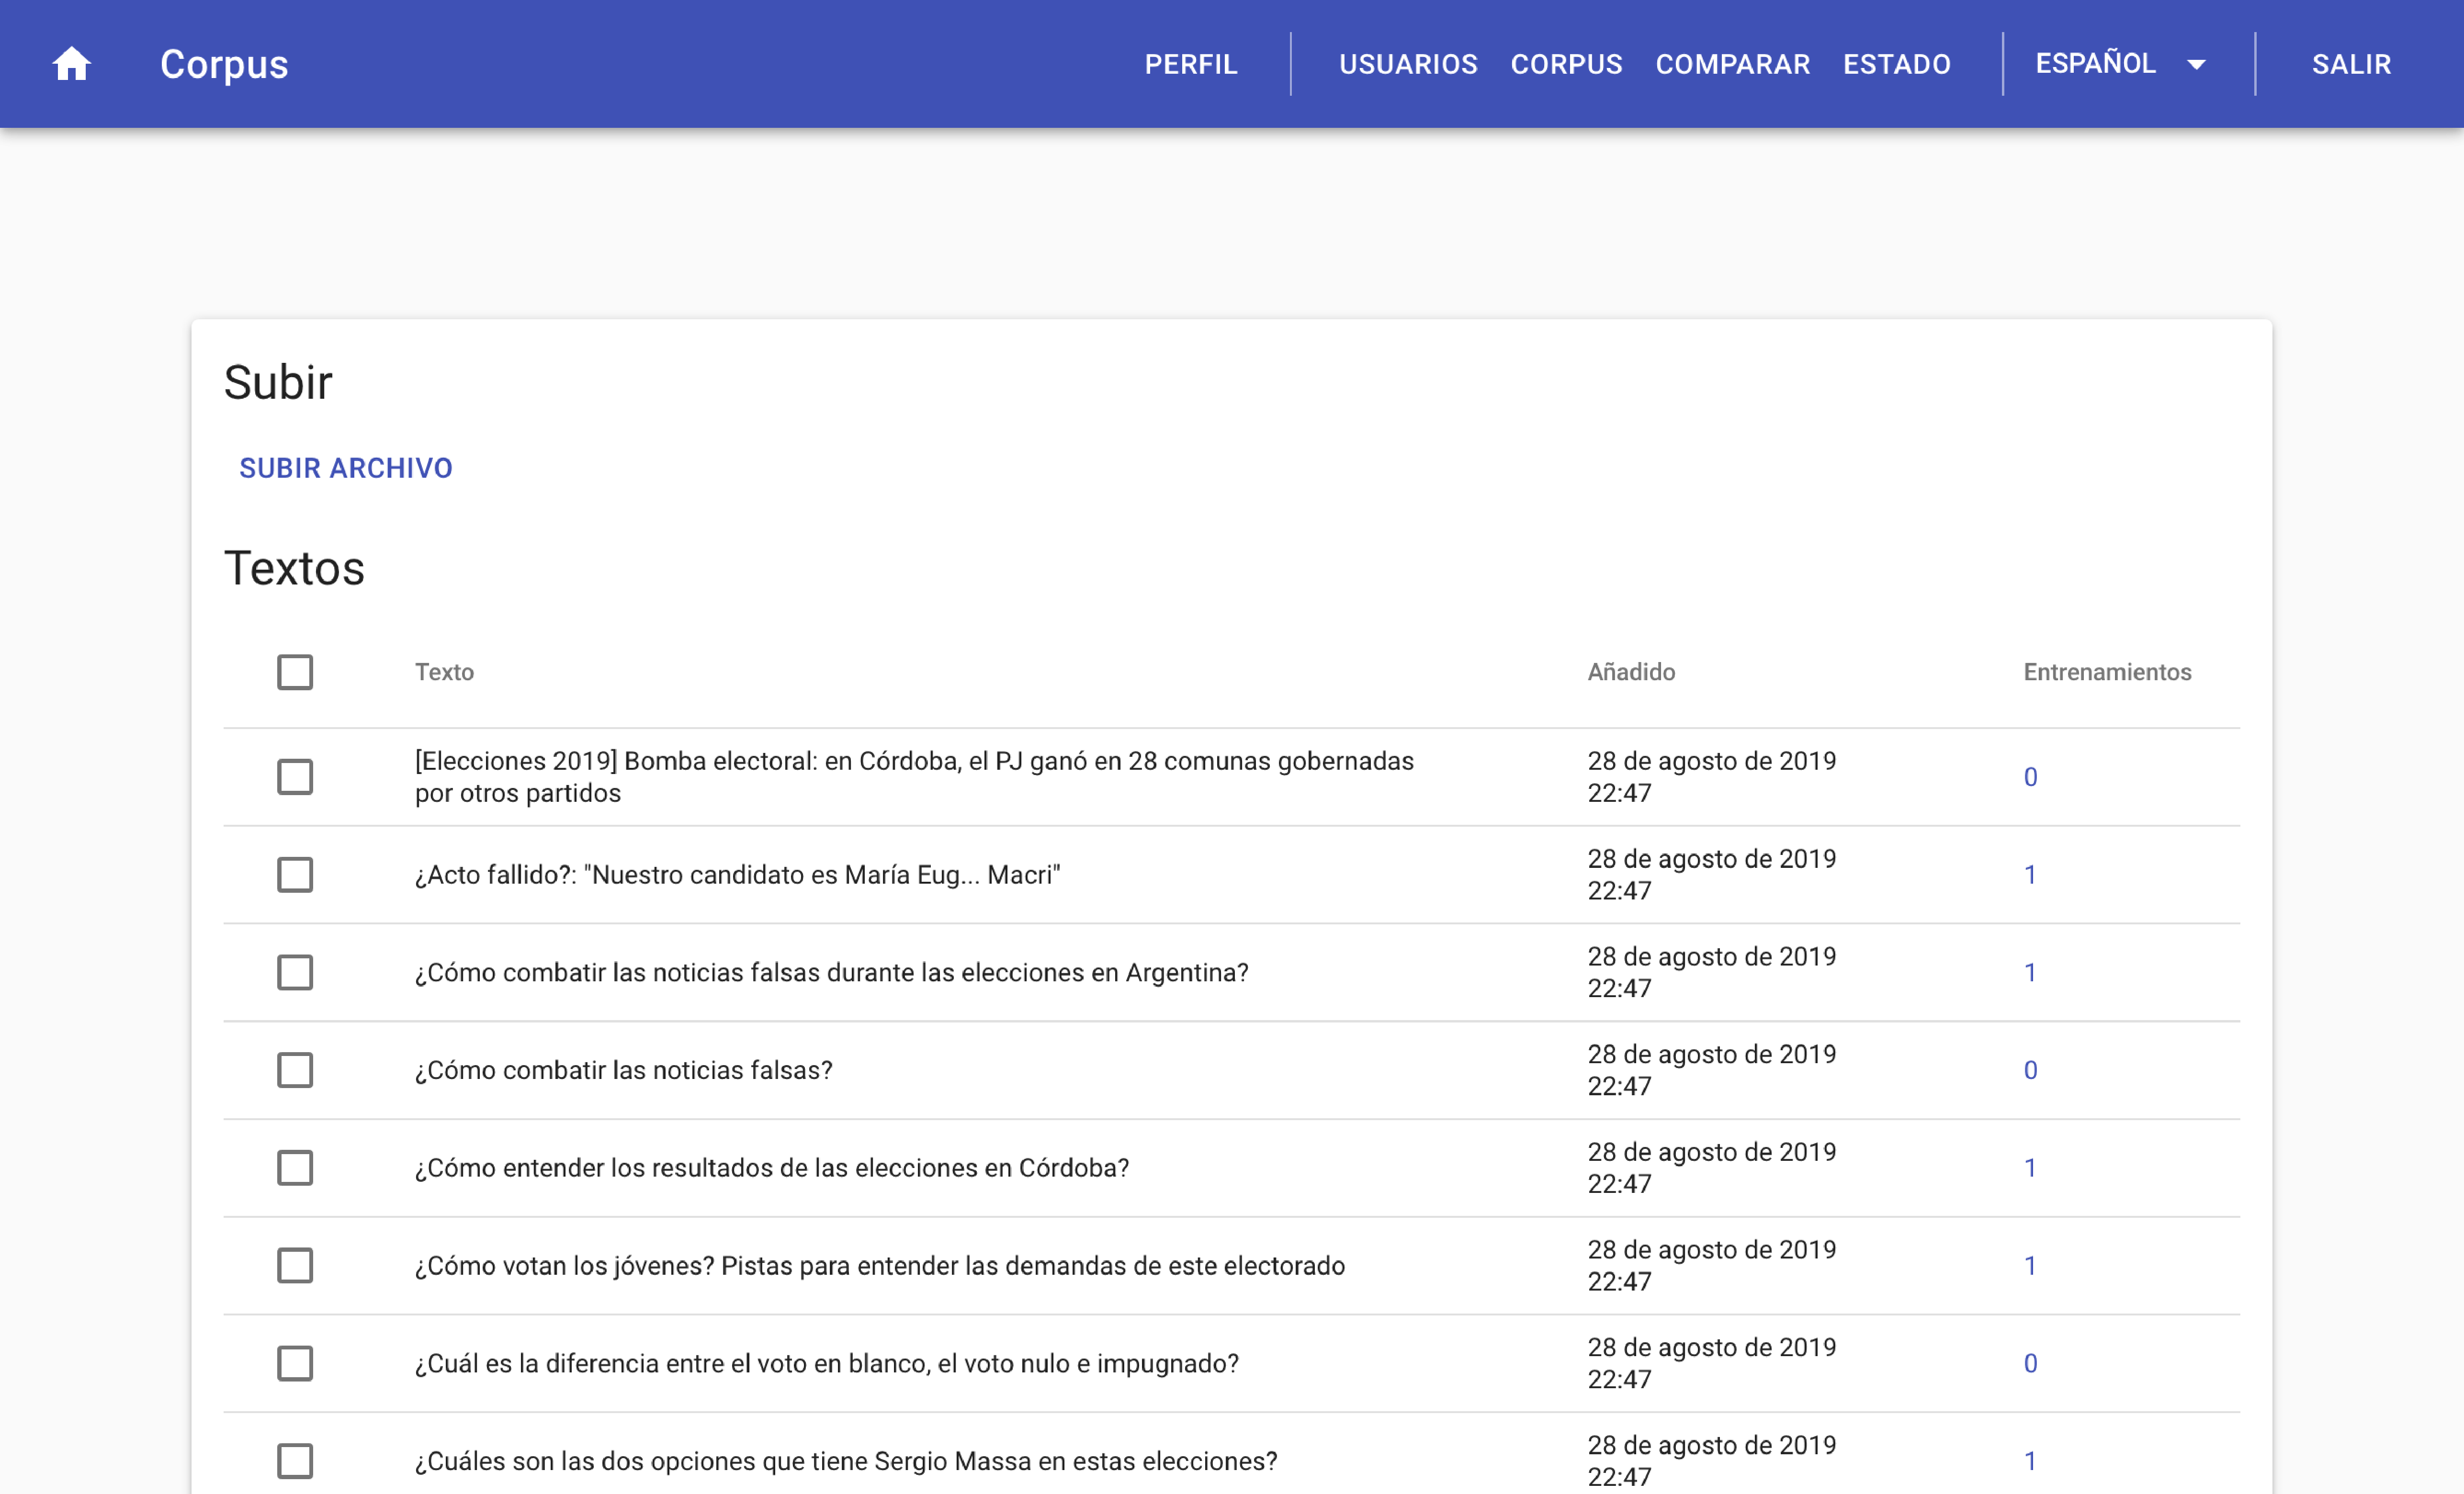
\includegraphics{assets/logic/corpus-management.pdf} 

}

\caption{Administración de corpus}\label{fig:logic-corpus-management}
\end{figure}

Desde aquí es posible agregar textos al corpus utilizando la funcionalidad de subida de archivos. Los archivos deben ser archivos con extensión \emph{.txt} y cada línea del archivo será agregada al corpus como un texto individual.

También es posible desde aquí ver todos los textos que forman parte del corpus así como también poder ver los entrenamientos para cada uno de los textos. Finalmente, es posible quitar textos del corpus así como también es posible eliminar correcciones a las inferencias de entidades cargados por usuarios.

\hypertarget{estado}{%
\paragraph{Estado}\label{estado}}

La pantalla de \emph{Estado} permite a un usuario con el rol de administrador visualizar el estado de entrenamiento del corpus así como también realizar diversas acciones sobre los \emph{workers}.

\begin{figure}[H]

{\centering 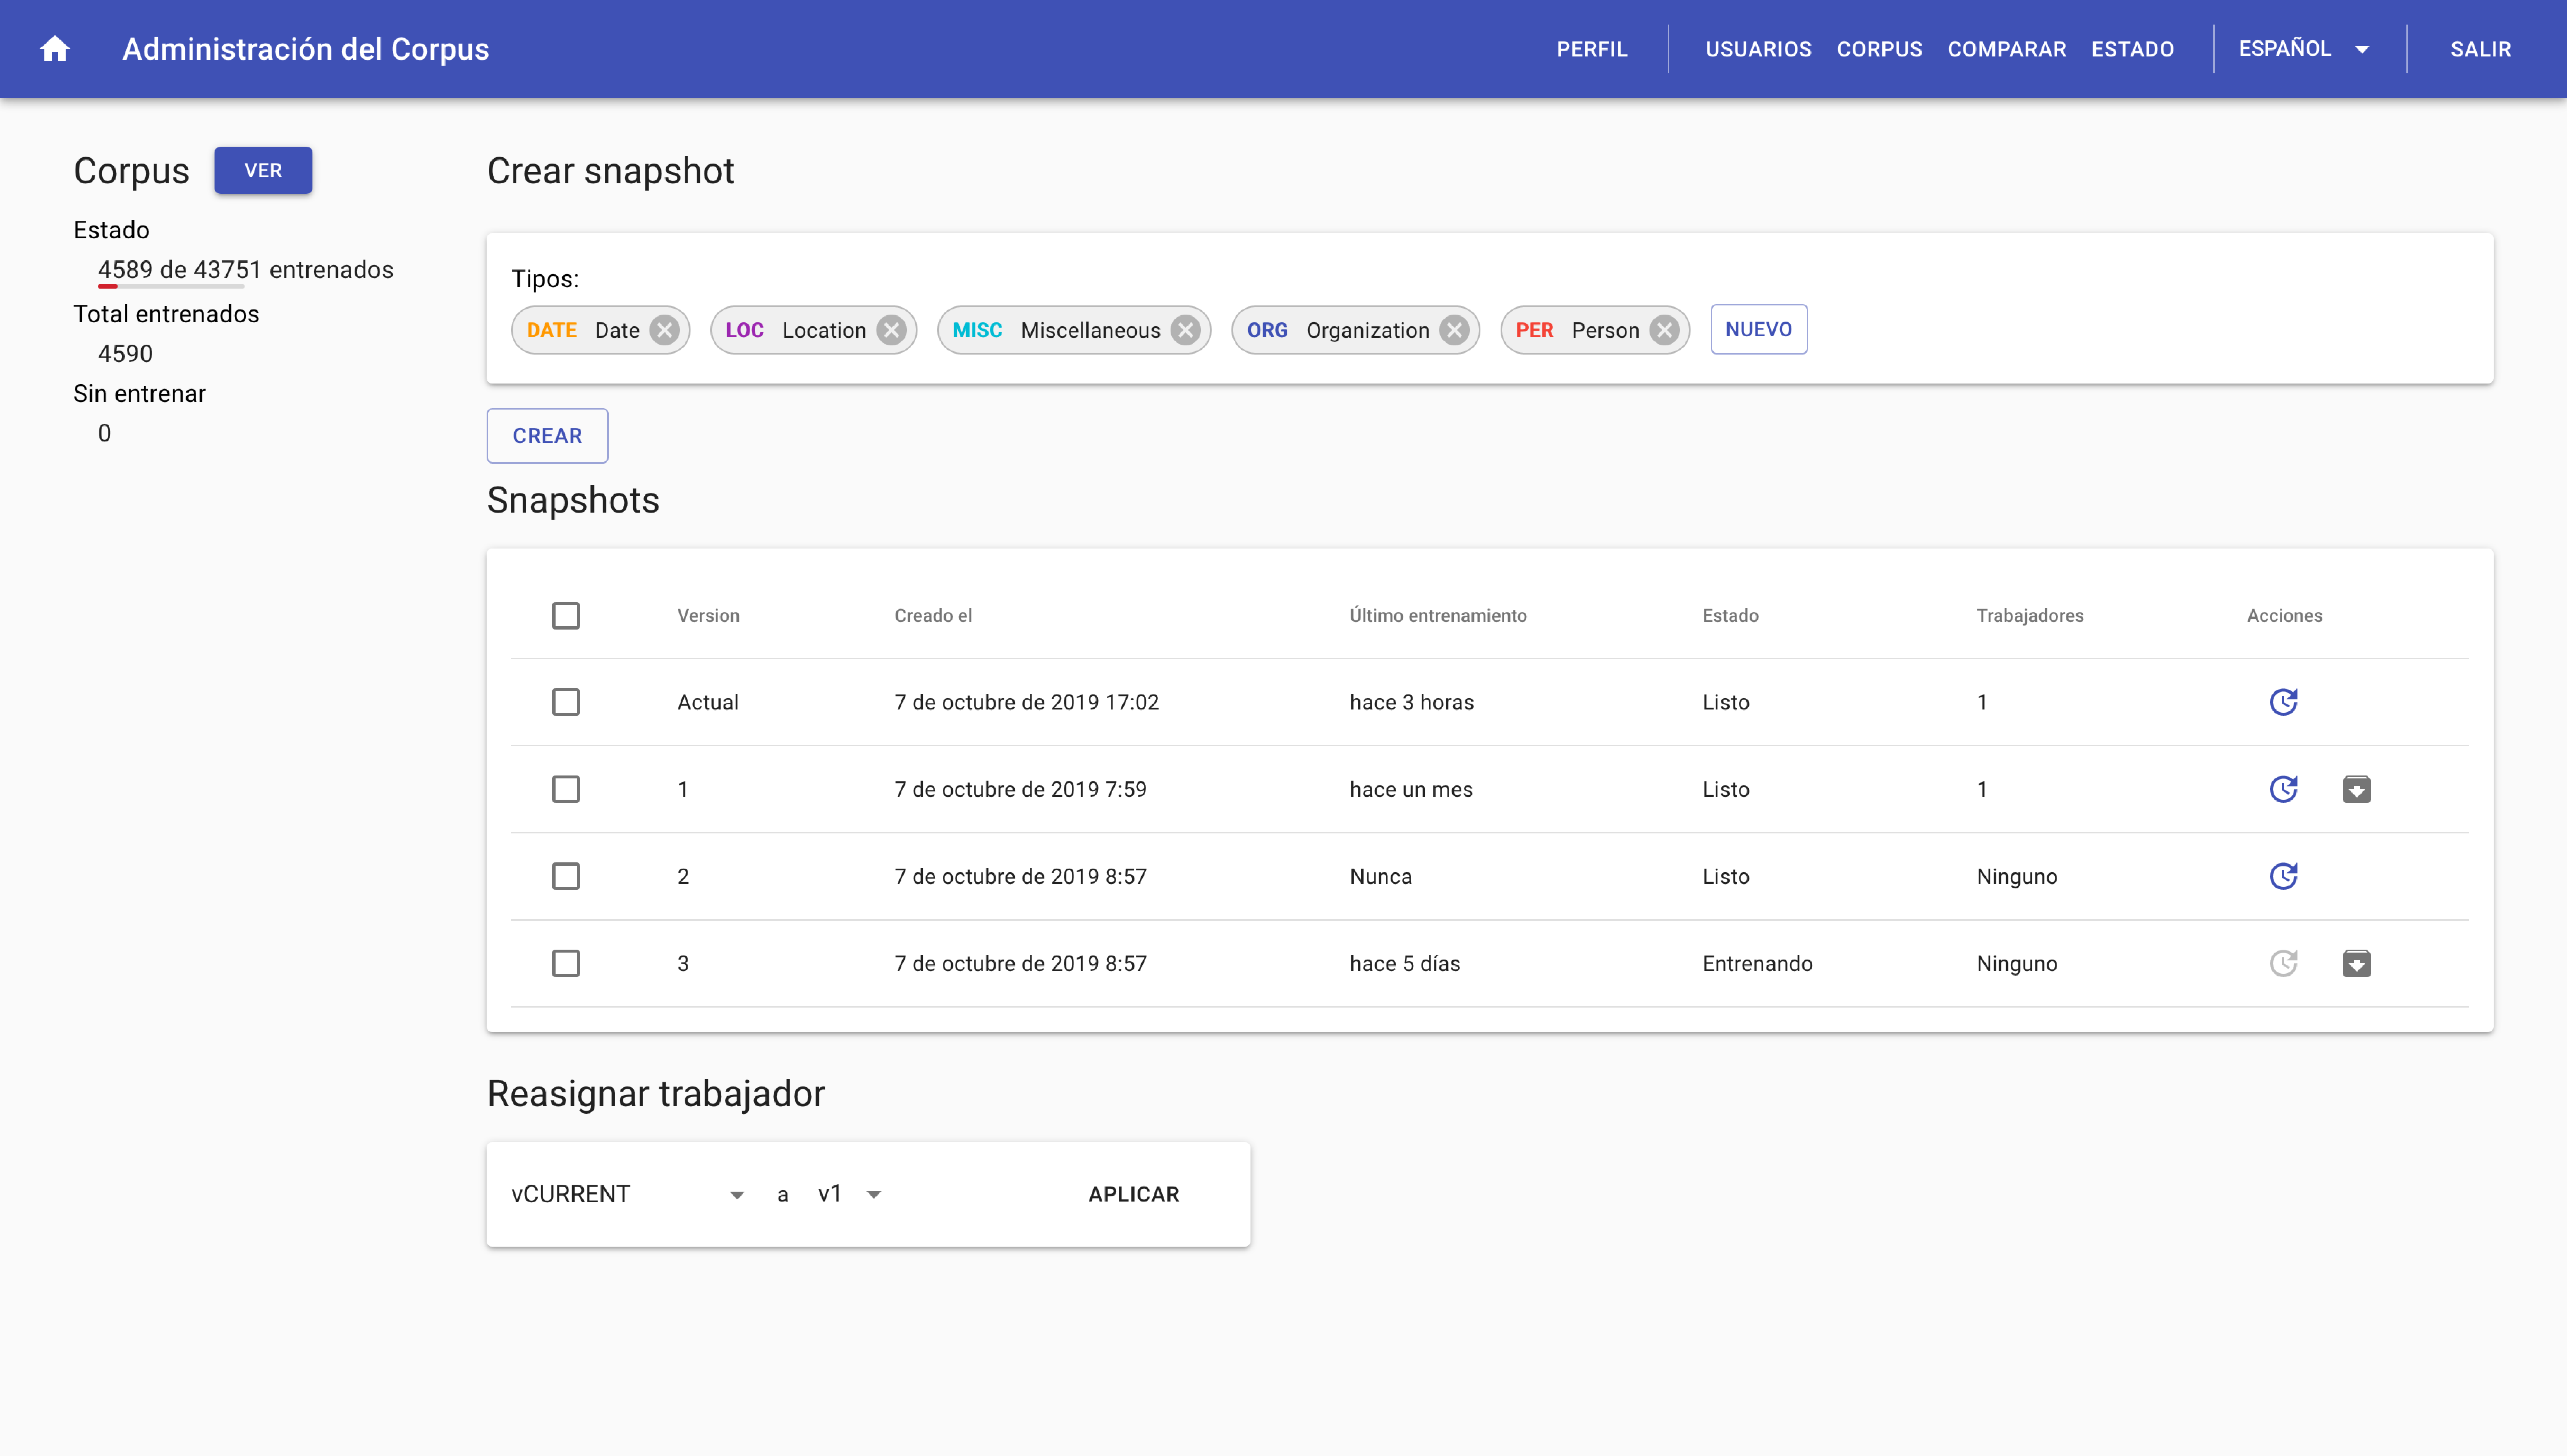
\includegraphics{assets/logic/status.pdf} 

}

\caption{Información de corpus y manejo de workers}\label{fig:logic-status}
\end{figure}

\hypertarget{secciones}{%
\subparagraph{Secciones}\label{secciones}}

Corpus

Es la columna la izquierda y aquí se puede ver rápidamente que porcentaje de el corpus contiene correcciones por usuarios así como también saber la cantidad total de correcciones del sistema (un texto puede tener más de una corrección por distintos usuarios) y también presenta un botón que permite al administrador ir a la pantalla de \emph{Corpus}.

Crear snapshot

Es la sección en la cual será posible crear, borrar o modificar los tipos de entidades reconocidos por el snapshot actual. La acción de editar las entidades genera un snapshot nuevo.

Si el administrador así lo quisiera, puede utilizar esta sección para crear un snapshot nuevo sin editar entidades.

Snapshots

Sección en la cual podemos ver la lista completa de snapshots.
Para cada Snapshot, se muestra cuando fue la última vez que se entrenó así como también cuantos trabajadores tiene asignados. Finalmente es posible desde aquí forzar a entrenar el modelo para ese snapshot en particular y también se presenta la opción para desentrenar, borrando el modelo guardado en el disco.

Reasignar trabajador

Sección que permite reasignar trabajadores para que sirvan un snapshot distinto. De esta manera se pueden servir distintas versiones del modelo de inferencia para poder realizar distintas pruebas sobre los mismos.

\hypertarget{sandbox}{%
\paragraph{Sandbox}\label{sandbox}}

La pantalla de \emph{Sandbox} permite a los usuarios hacer consultas al servicio NERd para poder obtener entidades nombradas a partir de textos arbitrarios.
Adicionalmente, si el usuario tiene el rol de entrenador, podrá corregir las entidades inferidas y agregar el texto con sus correcciones al corpus.

\begin{figure}[H]

{\centering 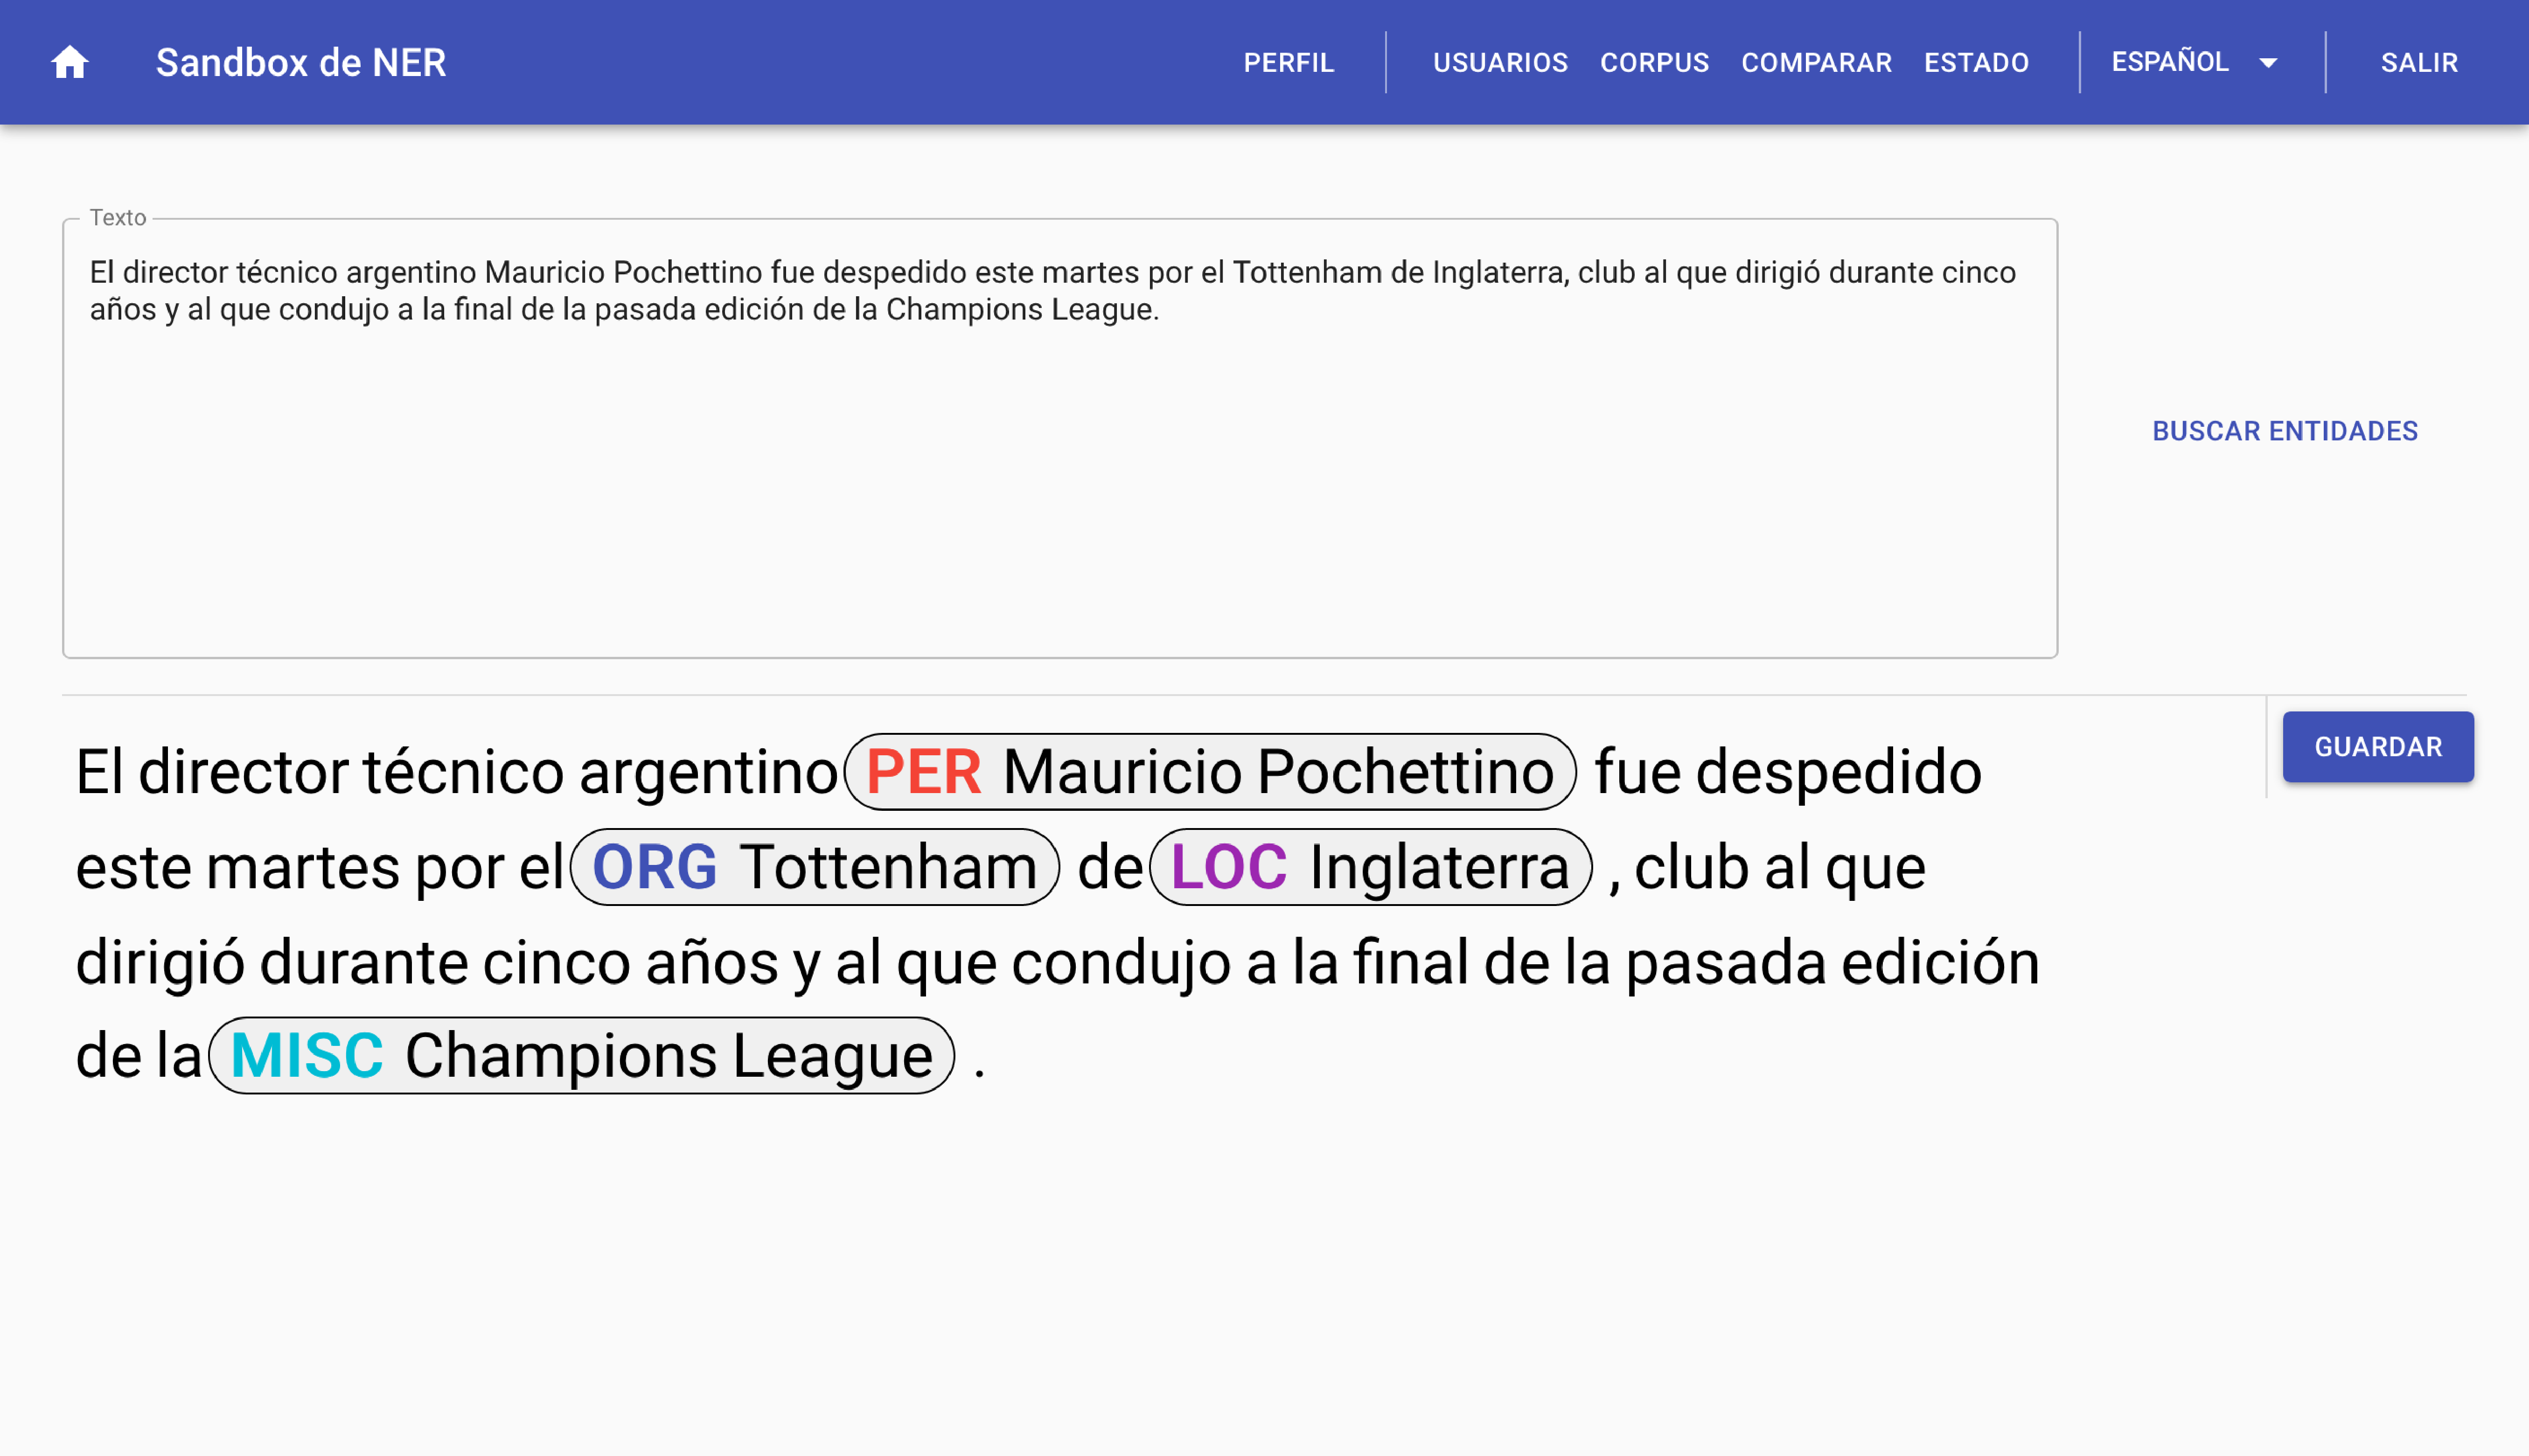
\includegraphics{assets/logic/sandbox.pdf} 

}

\caption{Inferencia de entidades en sandbox}\label{fig:logic-sandbox}
\end{figure}

\hypertarget{comparar}{%
\paragraph{Comparar}\label{comparar}}

Sección accesible únicamente a administradores en la que es posible comparar las entidades inferidas por dos modelos distintos. A su vez, si el usuario logueado tiene el permiso de entrenador, es posible corregir de manera inline los errores en la inferencia del modelo actual.

\begin{figure}[H]

{\centering 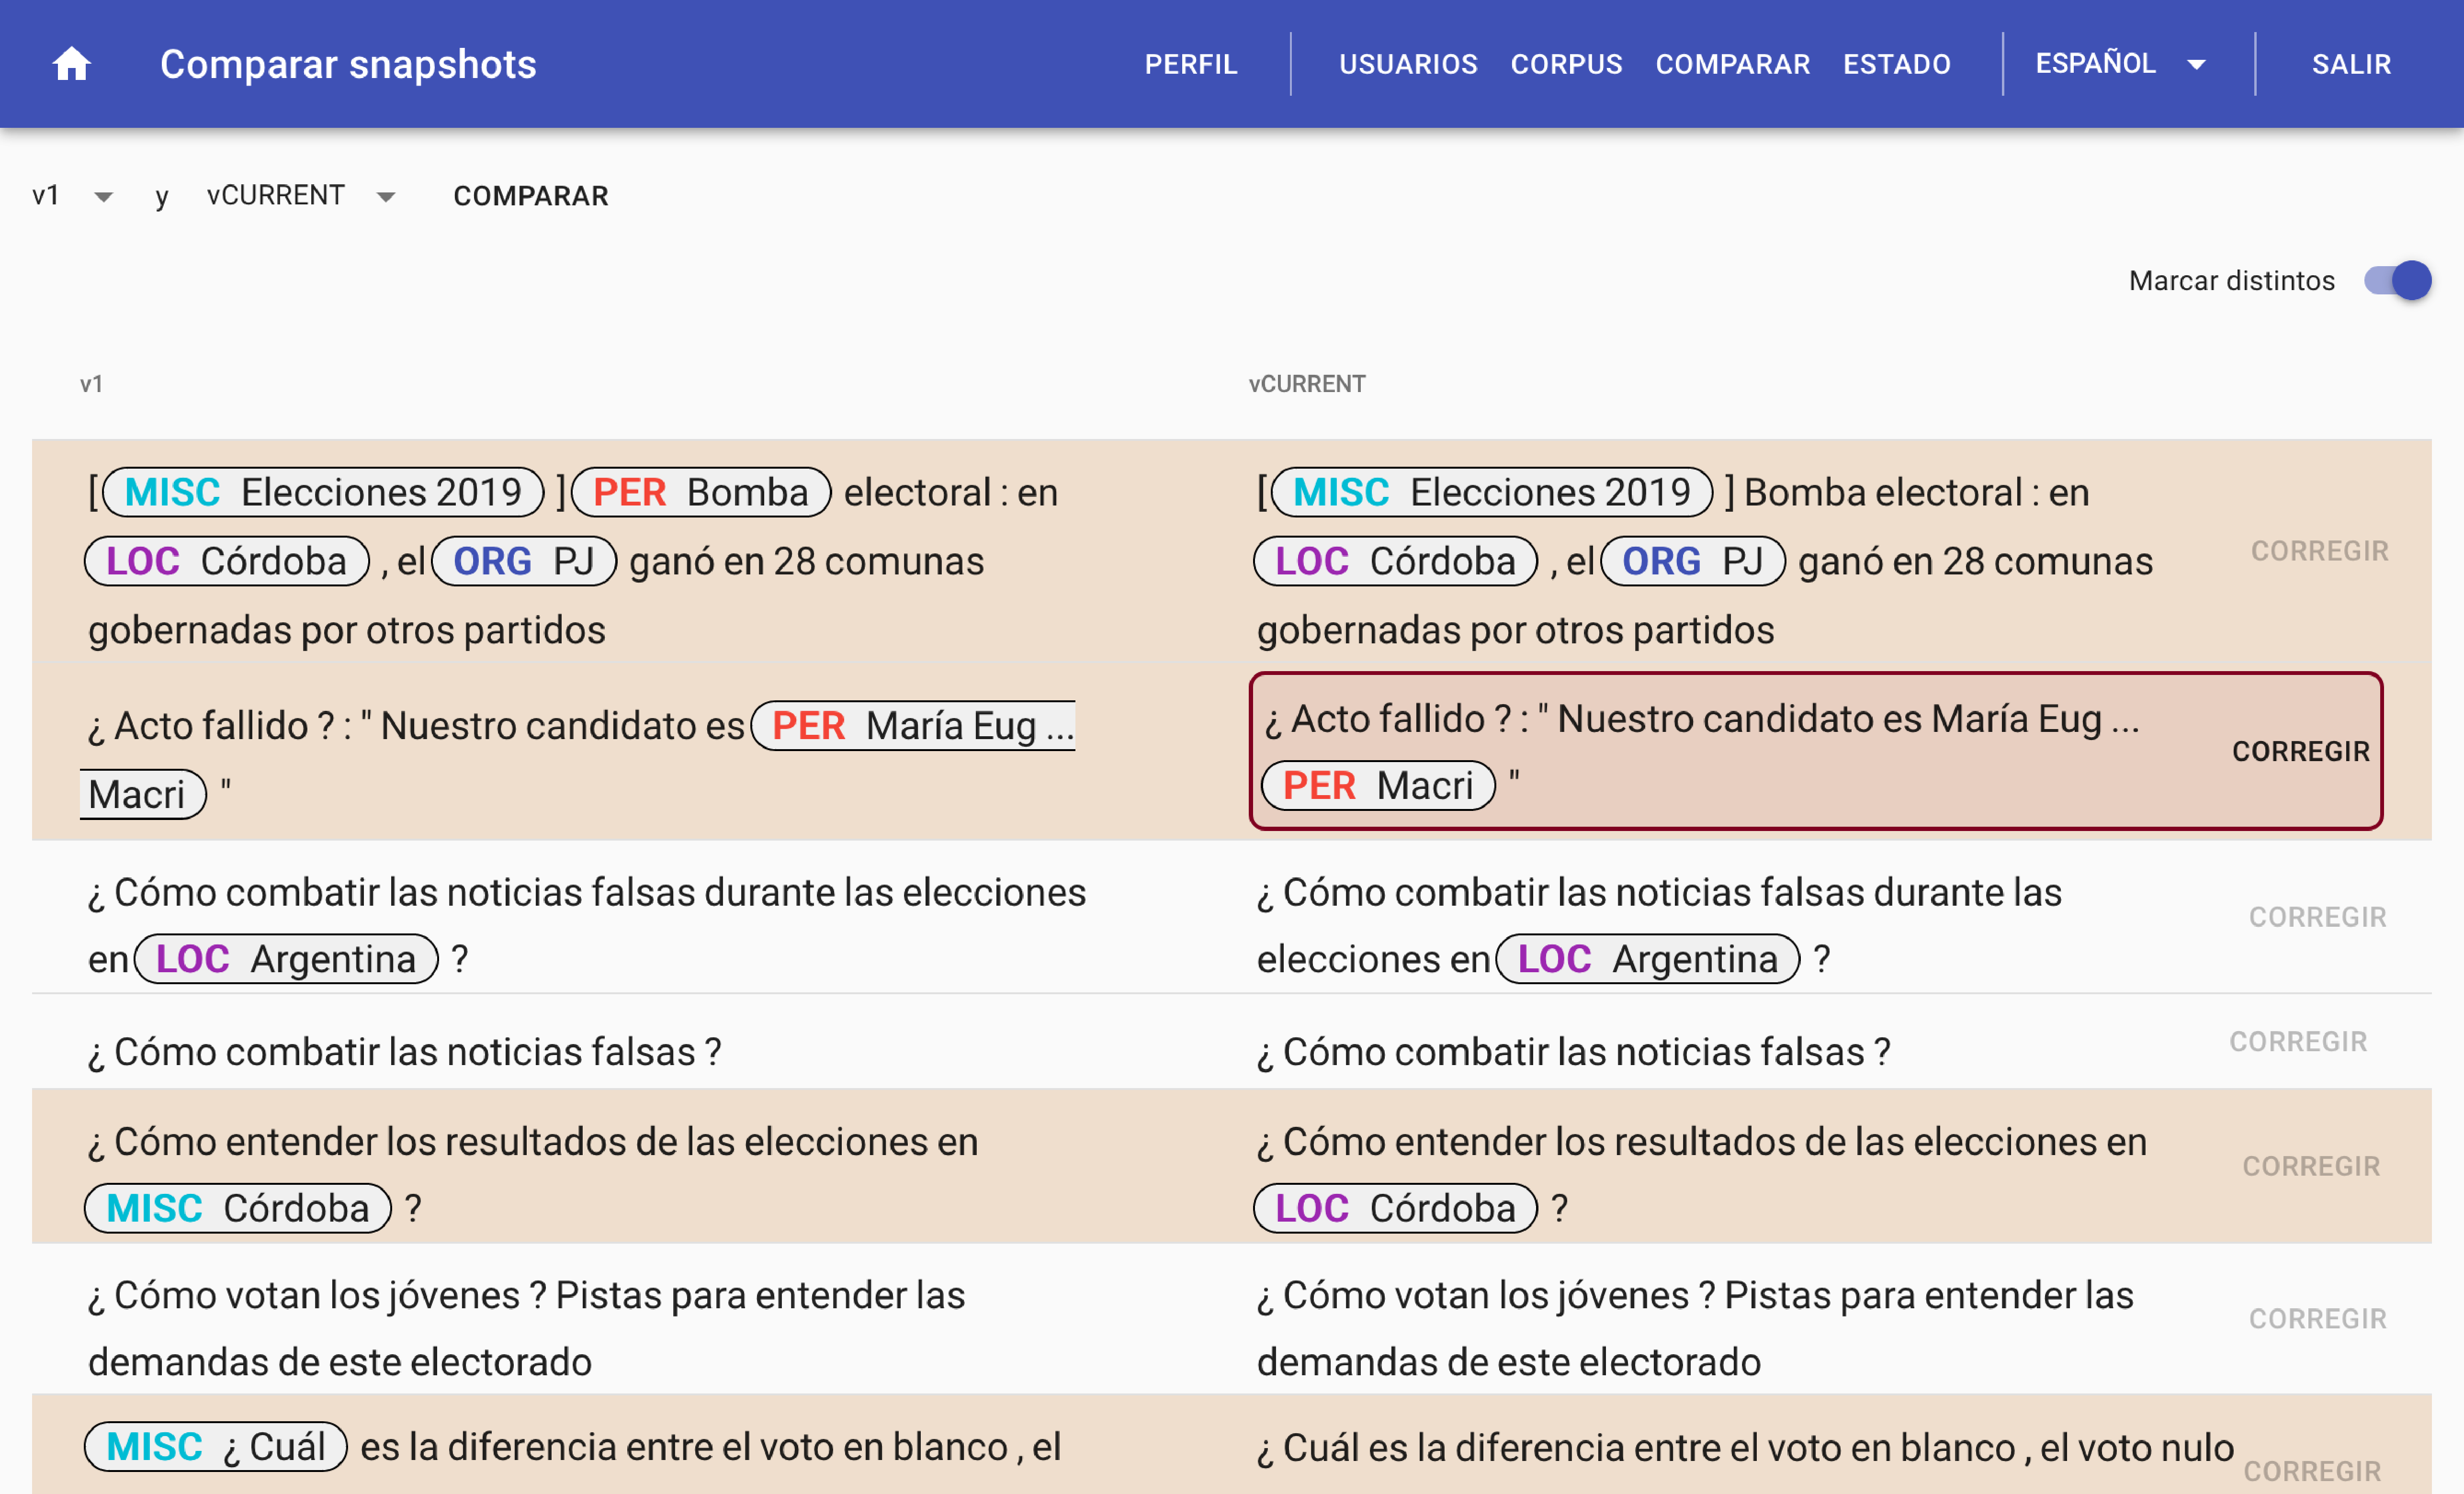
\includegraphics{assets/logic/compare.pdf} 

}

\caption{Comparativa de modelos}\label{fig:logic-compare}
\end{figure}

\hypertarget{vista-de-proceso}{%
\subsection{Vista de proceso}\label{vista-de-proceso}}

\begin{quote}
La vista de proceso trata los aspectos dinámicos del sistema, explica los procesos del sistema y cómo se comunican, y se centra en el comportamiento del sistema en tiempo de ejecución.
La vista de proceso aborda concurrencia, distribución, integradores, rendimiento y escalabilidad, etc.
\end{quote}

\hypertarget{vista-de-desarrollo}{%
\subsection{Vista de desarrollo}\label{vista-de-desarrollo}}

\begin{quote}
La vista de desarrollo ilustra un sistema desde la perspectiva de un programador y se ocupa de la gestión de software.
Esta vista también se conoce como la vista de implementación.
\end{quote}

\hypertarget{vista-fuxedsica}{%
\subsection{Vista física}\label{vista-fuxedsica}}

\begin{quote}
La vista física representa el sistema desde el punto de vista de un ingeniero de sistemas.
Se refiere a la topología de los componentes de software en la capa física, así como a las conexiones físicas entre estos componentes.
Esta vista también se conoce como la vista de \emph{deployment}.
\end{quote}

\hypertarget{escenarios}{%
\subsection{Escenarios}\label{escenarios}}

\begin{quote}
La descripción de una arquitectura se ilustra utilizando un pequeño conjunto de casos de uso, o escenarios, que se convierten en una quinta vista.
Los escenarios describen secuencias de interacciones entre objetos y entre procesos.
Se utilizan para identificar elementos arquitectónicos y para ilustrar y validar el diseño de la arquitectura.
También sirven como punto de partida para las pruebas de un prototipo de arquitectura.
Esta vista también se conoce como vista de caso de uso.
\end{quote}

\newpage

\hypertarget{results}{%
\section{Resultados}\label{results}}

Matriz de confusión -\textgreater{} dos indicadores!
true possitive vs true negative
Credibility: evaluation whats been leaerned.

\hypertarget{muxe9trica-precisiuxf3n-y-exhaustividad}{%
\subsection{Métrica: precisión y exhaustividad}\label{muxe9trica-precisiuxf3n-y-exhaustividad}}

(``Precision and recall,'' \protect\hyperlink{ref-wiki_Precision_and_recall}{2019})

\begin{quote}
TODO: reescribir

En conferencias académicas como CoNLL, se ha definido una variante del {[}{[}valor-F{]}{]} de la siguiente manera:

\begin{itemize}
\item
  Precisión es el número de entidades nombradas que coinciden exactamente con conjunto de evaluación. I.e. cuando se predice {[}Persona Hans{]} {[}Persona Blick{]}, pero lo correcto era {[}Person Hans Blick{]}, la precisión es cero. La precisión es después promediada por cada una de la entidades nombradas.
\item
  El recobrado es el número de entidades del conjunto de evaluación que aparecen exactamente en la misma posición en las predicciones.
\item
  El Valor-F es la media armónica de estos dos valores. Se deriva de la anterior definición que cualquier predicción que reconozca erróneamente un token como parte de una entidad nombrada o que deje de detectar un token que sí es una entidad nombrada o lo clasifique erróneamente no contribuirá ni a la precisión ni al recobrado.
\end{itemize}
\end{quote}

=== Evaluación formal ===
Para evaluar la calidad de la salida de un sistema NER, se han definido varias medidas. Las medidas habituales se llaman
{[}{[}Precision\_and\_recall \textbar{} Precisión, recuperación{]}{]} y {[}{[}Puntuación F1{]}{]}. Sin embargo, quedan varios problemas sobre cómo calcular esos valores.

Estas medidas estadísticas funcionan razonablemente bien para los casos obvios de encontrar o faltar una entidad real exactamente; y para encontrar una no entidad. Sin embargo, NER puede fallar de muchas otras maneras, muchas de las cuales son posiblemente \enquote{parcialmente correctas}, y no deben considerarse como éxitos o fracasos competitivos. Por ejemplo, identificar una entidad real, pero:
* con menos tokens de los deseados (por ejemplo, falta el último token de \enquote{John Smith, M.D.})
* con más tokens de los deseados (por ejemplo, incluyendo la primera palabra de \enquote{The University of MD})
* particionando entidades adyacentes de manera diferente (por ejemplo, tratando a \enquote{Smith, Jones Robinson} como entidades 2 vs.~3)
* asignarle un tipo completamente incorrecto (por ejemplo, llamar a un nombre personal a una organización)
* asignándole un tipo relacionado pero inexacto (por ejemplo, \enquote{sustancia} vs. \enquote{droga}, o \enquote{escuela} vs. \enquote{organización})
* identificar correctamente una entidad, cuando lo que el usuario quería era una entidad de menor o mayor alcance (por ejemplo, identificar \enquote{James Madison} como un nombre personal, cuando forma parte de la \enquote{Universidad James Madison}. Algunos sistemas NER imponen la restricción que las entidades nunca se superpongan o aniden, lo que significa que en algunos casos uno debe tomar decisiones arbitrarias o específicas de la tarea.

Un método demasiado simple para medir la precisión es simplemente contar qué fracción de todas las fichas en el texto se identificaron correcta o incorrectamente como parte de referencias de entidad (o como entidades del tipo correcto). Esto tiene al menos dos problemas: en primer lugar, la gran mayoría de los tokens en el texto del mundo real no forman parte de los nombres de las entidades, por lo que la precisión de la línea de base (siempre predice \enquote{no una entidad}) es extravagantemente alta, típicamente\textgreater{} 90\%; y segundo, predecir erróneamente el lapso completo del nombre de una entidad no se penaliza adecuadamente (encontrar solo el nombre de una persona cuando le sigue su apellido podría calificarse como ½ precisión).

En conferencias académicas como CoNLL, una variante de la {[}{[}puntuación F1{]}{]} se ha definido de la siguiente manera: \{\{r \textbar{} conll03intro\}\}

\begin{itemize}
\tightlist
\item
  {[}{[}Precisión y recuperación \textbar{} Precisión{]}{]} es el número de intervalos de nombre de entidad pronosticados que se alinean '' exactamente '' con intervalos en los datos de evaluación {[}{[}Verdad fundamental \# Estadísticas y aprendizaje automático \textbar{} estándar de oro{]}{]}. Es decir. cuando se predice {[} Persona Hans{]} {[} Persona Blick{]} pero se requiere {[} Persona Hans Blick{]}, la precisión del nombre predicho es cero. La precisión se promedia sobre todos los nombres de entidad pronosticados.
\item
  Recordar es igualmente el número de nombres en el estándar de oro que aparecen exactamente en la misma ubicación en las predicciones.
\item
  La puntuación F1 es la {[}{[}media armónica{]}{]} de estos dos.
\end{itemize}

De la definición anterior se deduce que cualquier predicción que omita un solo token, incluye un token espurio o tiene clase incorrecta, es un error difícil y no contribuye positivamente ni a la precisión ni a la recuperación. Por lo tanto, se puede decir que esta medida es pesimista: puede darse el caso de que muchos \enquote{errores} estén cerca de ser correctos, y podrían ser adecuados para un propósito dado. Por ejemplo, un sistema siempre puede omitir títulos como \enquote{Sra.} o \enquote{Ph.D.}, pero se compara con un sistema o datos de verdad que esperan que se incluyan títulos. En esos casos, cada nombre se trata como un error. Debido a tales problemas, es importante examinar los tipos de errores y decidir qué tan importantes se les dan los objetivos y requisitos.

\newpage

\hypertarget{discussion}{%
\section{Discusión}\label{discussion}}

\hypertarget{tipos-de-entidades-relevantes}{%
\subsection{Tipos de entidades relevantes}\label{tipos-de-entidades-relevantes}}

tener en cuenta (Brunstein, \protect\hyperlink{ref-brunstein2002}{2002})

\begin{verbatim}
# Notas sobre mejora en tipos de entidades
Presidente -> Person Descriptor
NORP -> (Polical) Peronistas, Kirchneristas
Facility Name -> usually location. "Wall Street", "Muralla China"

Organization Name -> Government vs Corporation.
Product Name -> autos "Fiat Toro", celulares "Galaxy S10"
Events -> Superclásico. Superliga. Copa argentina. Elecciones 2019. Las Paso.
Disease -> 
Game -> Football, Basket (para "titulos" no tan relevante)
\end{verbatim}

\hypertarget{seed-en-los-types}{%
\subsection{Seed en los types}\label{seed-en-los-types}}

en especial para los nuevos.

\hypertarget{linkeo-de-entidades-con-knowledge-base}{%
\subsection{Linkeo de entidades con Knowledge Base}\label{linkeo-de-entidades-con-knowledge-base}}

La tarea de reconocer entidades nombradas en el texto es Reconocimiento de entidades nombradas, mientras que la tarea de determinar la identidad de las entidades nombradas mencionadas en el texto se llama Desambiguación de entidades nombradas. Ambas tareas requieren algoritmos y recursos dedicados para ser abordados. {[}3{]}

\hypertarget{mejora-live-vs-offline}{%
\subsection{Mejora live vs offline}\label{mejora-live-vs-offline}}

Mejora \enquote{Uncertainty sampling} -\textgreater{} buscar entidades que tengan un score \textasciitilde{} 0.5

\hypertarget{utilidad-de-la-herramienta}{%
\subsection{Utilidad de la herramienta}\label{utilidad-de-la-herramienta}}

Para poder poner a prueba nuestra herramienta \textbf{NERd} en un entorno real participamos de la hackaton en MediaParty 2019.

\begin{quote}
\textbf{(``Hackaton,'' \protect\hyperlink{ref-hackaton2019}{2019})} es un evento de tres días en Argentina, que reúne a 2500 emprendedores, periodistas, programadores de software y diseñadores de cinco continentes para trabajar juntos para el futuro de los medios de comunicación.
Nacido de Hacks/Hackers Buenos Aires, el evento fusiona a grandes empresas como New York Times, The Guardian, Vox, ProPublica, Watchup, Neo4J o DocumentCloud y comunidades regionales de la mayor red de periodistas y desarrolladores del mundo.
\end{quote}

Participamos en conjunto con otro proyecto final en el que van a utilizar nuestra API para hacer detección de entidades en documentos PDF.

La experiencia fue muy satisfactoria, recibimos buenas críticas sobre la Usabilidad de nuestra aplicación y la gran utilidad que presta a la comunidad.

Por tal motivo recibimos el primer premio de dicha hackaton (``Mención itba,'' \protect\hyperlink{ref-mediaparty2019_win}{2019})

\newpage

\hypertarget{conclusiones}{%
\section{Conclusiones}\label{conclusiones}}

\hypertarget{examples}{%
\subsection{Examples}\label{examples}}

You can label chapter and section titles using \texttt{\{\#label\}} after them, e.g., we can reference Chapter \ref{intro}. If you do not manually label them, there will be automatic labels anyway, e.g., Chapter \ref{state-of-art}.

Figures and tables with captions will be placed in \texttt{figure} and \texttt{table} environments, respectively.

\begin{Shaded}
\begin{Highlighting}[]
\KeywordTok{par}\NormalTok{(}\DataTypeTok{mar =} \KeywordTok{c}\NormalTok{(}\DecValTok{4}\NormalTok{, }\DecValTok{4}\NormalTok{, }\FloatTok{.1}\NormalTok{, }\FloatTok{.1}\NormalTok{))}
\KeywordTok{plot}\NormalTok{(pressure, }\DataTypeTok{type =} \StringTok{'b'}\NormalTok{, }\DataTypeTok{pch =} \DecValTok{19}\NormalTok{)}
\end{Highlighting}
\end{Shaded}

\begin{figure}

{\centering 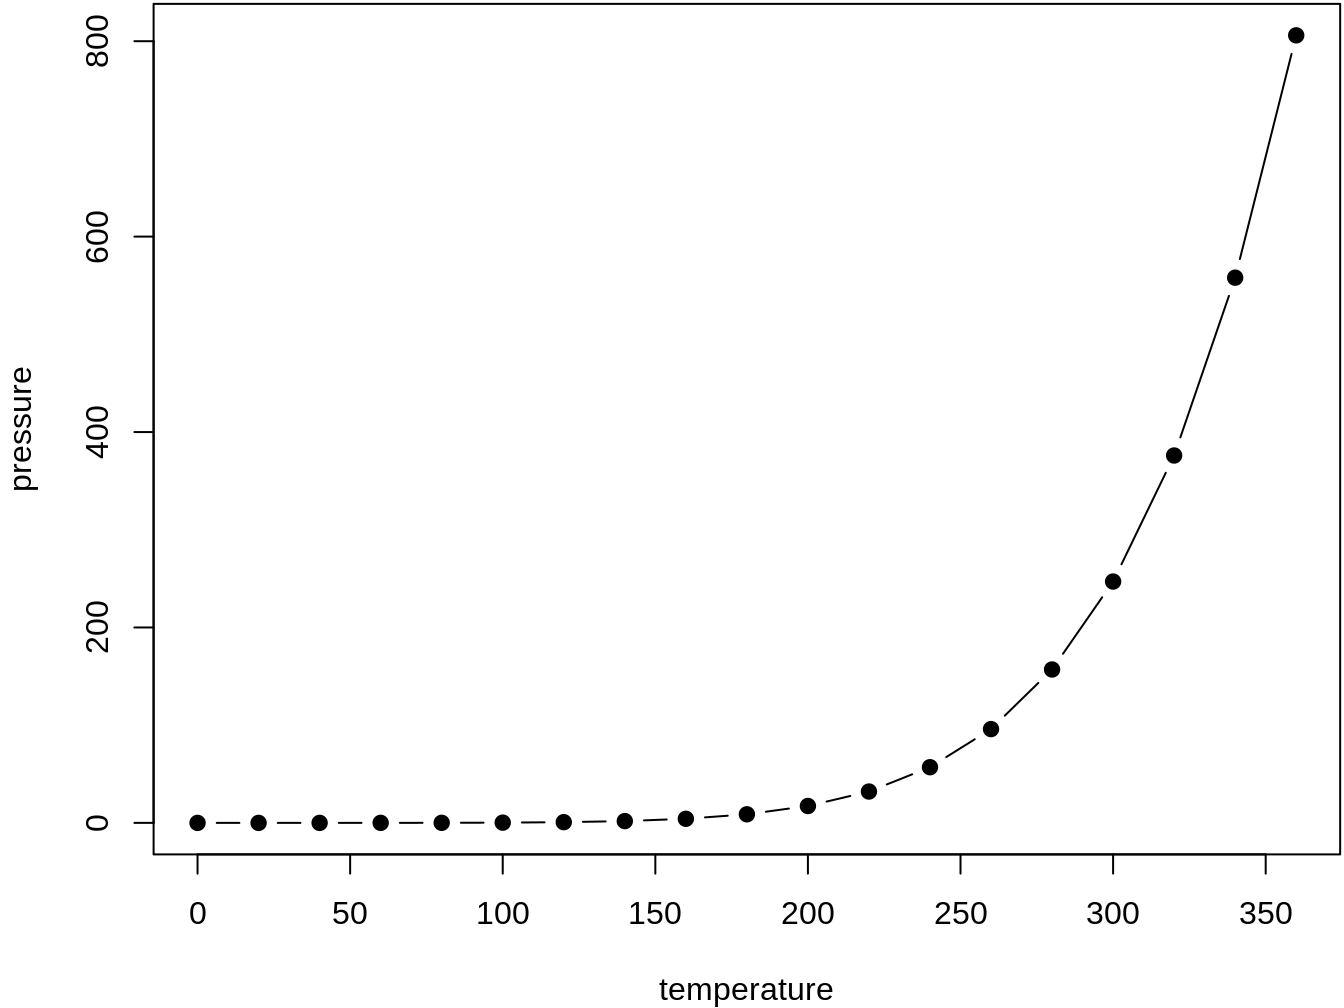
\includegraphics[width=0.8\linewidth]{nerd-pf_files/figure-latex/nice-fig-1.pdf} 

}

\caption{Here is a nice figure!}\label{fig:nice-fig}
\end{figure}

Reference a figure by its code chunk label with the \texttt{fig:} prefix, e.g., see Figure \ref{fig:nice-fig}. Similarly, you can reference tables generated from \texttt{knitr::kable()}, e.g., see Table \ref{tab:nice-tab}.

\begin{Shaded}
\begin{Highlighting}[]
\NormalTok{knitr}\OperatorTok{::}\KeywordTok{kable}\NormalTok{(}
  \KeywordTok{head}\NormalTok{(iris, }\DecValTok{20}\NormalTok{), }\DataTypeTok{caption =} \StringTok{'Here is a nice table!'}\NormalTok{,}
  \DataTypeTok{booktabs =} \OtherTok{TRUE}
\NormalTok{)}
\end{Highlighting}
\end{Shaded}

\begin{table}

\caption{\label{tab:nice-tab}Here is a nice table!}
\centering
\begin{tabular}[t]{rrrrl}
\toprule
Sepal.Length & Sepal.Width & Petal.Length & Petal.Width & Species\\
\midrule
5.1 & 3.5 & 1.4 & 0.2 & setosa\\
4.9 & 3.0 & 1.4 & 0.2 & setosa\\
4.7 & 3.2 & 1.3 & 0.2 & setosa\\
4.6 & 3.1 & 1.5 & 0.2 & setosa\\
5.0 & 3.6 & 1.4 & 0.2 & setosa\\
\addlinespace
5.4 & 3.9 & 1.7 & 0.4 & setosa\\
4.6 & 3.4 & 1.4 & 0.3 & setosa\\
5.0 & 3.4 & 1.5 & 0.2 & setosa\\
4.4 & 2.9 & 1.4 & 0.2 & setosa\\
4.9 & 3.1 & 1.5 & 0.1 & setosa\\
\addlinespace
5.4 & 3.7 & 1.5 & 0.2 & setosa\\
4.8 & 3.4 & 1.6 & 0.2 & setosa\\
4.8 & 3.0 & 1.4 & 0.1 & setosa\\
4.3 & 3.0 & 1.1 & 0.1 & setosa\\
5.8 & 4.0 & 1.2 & 0.2 & setosa\\
\addlinespace
5.7 & 4.4 & 1.5 & 0.4 & setosa\\
5.4 & 3.9 & 1.3 & 0.4 & setosa\\
5.1 & 3.5 & 1.4 & 0.3 & setosa\\
5.7 & 3.8 & 1.7 & 0.3 & setosa\\
5.1 & 3.8 & 1.5 & 0.3 & setosa\\
\bottomrule
\end{tabular}
\end{table}

You can write citations, too. For example, we are using the \textbf{bookdown} package (Xie, \protect\hyperlink{ref-R-bookdown}{2019}) in this sample book, which was built on top of R Markdown and \textbf{knitr} (Xie, \protect\hyperlink{ref-xie2015}{2015}).

\newpage

\hypertarget{refs}{}
\leavevmode\hypertarget{ref-brunstein2002}{}%
Brunstein, A. (2002). Annotation guidelines for answer types. Retrieved from \url{https://catalog.ldc.upenn.edu/docs/LDC2005T33/BBN-Types-Subtypes.html}

\leavevmode\hypertarget{ref-cambridge_duh}{}%
Duh definition. (2019). Retrieved October 14, 2019, from \url{https://dictionary.cambridge.org/es/diccionario/ingles/duh}

\leavevmode\hypertarget{ref-ethayarajh-etal-2019-towards}{}%
Ethayarajh, K., Duvenaud, D., \& Hirst, G. (2019). Towards understanding linear word analogies. \emph{Proceedings of the 57th annual meeting of the association for computational linguistics}, 3253--3262. \url{https://doi.org/10.18653/v1/P19-1315}

\leavevmode\hypertarget{ref-hackaton2019}{}%
Hackaton. (2019). Retrieved August 31, 2019, from \url{https://mediaparty.info/}

\leavevmode\hypertarget{ref-honnibal_NER}{}%
Honnibal, M. (2017). Practical and effective neural ner. Retrieved November 2, 2017, from \url{https://github.com/explosion/talks/blob/master/2017-11-02_Practical-and-Effective-Neural-NER.pdf}

\leavevmode\hypertarget{ref-kripke1980naming}{}%
Kripke, S. (1980). \emph{Naming and necessity}. Retrieved from \url{https://books.google.com.ar/books?id=9vvAlOBfq0kC}

\leavevmode\hypertarget{ref-Kruchten:1995:VMA:624610.625529}{}%
Kruchten, P. (1995). The 4+1 view model of architecture. \emph{IEEE Softw.}, \emph{12}(6), 42--50. \url{https://doi.org/10.1109/52.469759}

\leavevmode\hypertarget{ref-DBLP:journalsux2fcorrux2fLampleBSKD16}{}%
Lample, G., Ballesteros, M., Subramanian, S., Kawakami, K., \& Dyer, C. (2016). Neural architectures for named entity recognition. \emph{CoRR}, \emph{abs/1603.01360}. Retrieved from \url{http://arxiv.org/abs/1603.01360}

\leavevmode\hypertarget{ref-marsh-perzanowski-1998-muc}{}%
Marsh, E., \& Perzanowski, D. (1998). MUC-7 evaluation of IE technology: Overview of results. \emph{Seventh message understanding conference (MUC-7): Proceedings of a conference held in fairfax, virginia, April 29 - may 1, 1998}. Retrieved from \url{https://www.aclweb.org/anthology/M98-1002}

\leavevmode\hypertarget{ref-mediaparty2019_win}{}%
Mención itba. (2019). Retrieved October 3, 2019, from \url{https://www.instagram.com/p/B3Koum2peD-/}

\leavevmode\hypertarget{ref-montani_AI}{}%
Montani, I. (2016). Practical and effective neural ner. Retrieved November 28, 2016, from \url{https://github.com/explosion/talks/blob/master/2016-11-28_The-State-of-AI-2016.pdf}

\leavevmode\hypertarget{ref-Poibeau2000ProperNE}{}%
Poibeau, T., \& Kosseim, L. (2000). Proper name extraction from non-journalistic texts. \emph{CLIN}.

\leavevmode\hypertarget{ref-wiki_Precision_and_recall}{}%
Precision and recall. (2019). Retrieved October 16, 2019, from \url{https://en.wikipedia.org/wiki/Precision_and_recall}

\leavevmode\hypertarget{ref-github_machine_learning}{}%
The state of the octoverse: Machine learning. (2019). Retrieved January 24, 2019, from \url{https://github.blog/2019-01-24-the-state-of-the-octoverse-machine-learning/}

\leavevmode\hypertarget{ref-xie2015}{}%
Xie, Y. (2015). \emph{Dynamic documents with R and knitr} (2nd ed.). Retrieved from \url{http://yihui.name/knitr/}

\leavevmode\hypertarget{ref-R-bookdown}{}%
Xie, Y. (2019). \emph{Bookdown: Authoring books and technical documents with r markdown}. Retrieved from \url{https://github.com/rstudio/bookdown}


\end{document}
